% !Mode:: "TeX:UTF-8"
% !TEX encoding = UTF-8 Unicode

%----------------------------------------------------------------------------------------
% 机器翻译:统计建模与深度学习方法
% Machine Translation: Statistical Modeling and Deep Learning Methods
%
% Copyright 2020
% 肖桐(xiaotong@mail.neu.edu.cn) 朱靖波 (zhujingbo@mail.neu.edu.cn)
%----------------------------------------------------------------------------------------

%----------------------------------------------------------------------------------------
%    CONFIGURATIONS
%----------------------------------------------------------------------------------------

\renewcommand\figurename{图} % Figure => 图
\renewcommand\tablename{表}% Table => 表
\definecolor{ublue}{rgb}{0.152,0.250,0.545} % Color of deep blue
\definecolor{ugreen}{rgb}{0,0.5,0} % Color of deep green
\chapterimage{fig-NEU-4.jpg} % Chapter heading image

%----------------------------------------------------------------------------------------
%	PART 2
%----------------------------------------------------------------------------------------

\part{统计机器翻译}

%----------------------------------------------------------------------------------------
%	CHAPTER 3
%----------------------------------------------------------------------------------------

\chapter{基于词的机器翻译模型}

\parinterval 使用概率化的方法对翻译问题进行建模是机器翻译发展中的重要里程碑。这种思想也影响了当今的统计机器翻译和神经机器翻译方法。虽然技术不断发展,传统的统计模型已经不再``新鲜'',但它对于今天机器翻译的研究仍然有着重要的启示作用。在了解前沿、展望未来的同时,我们更要冷静的思考前人给我们带来了什么。基于此,本章将介绍统计机器翻译的开山之作\ \dash \ IBM模型,它提出了使用统计模型进行翻译的思想,并在建模中引入了单词对齐这一重要概念。IBM模型由Peter F. Brown等人于上世纪九十年代初提出\cite{Peter1993The}。客观的说,这项工作的视野和对问题的理解,已经超过当时很多人所能看到的东西,其衍生出来的一系列方法和新的问题还被后人花费将近10年的时间来进行研究与讨论。时至今日,IBM模型中的一些思想仍然影响着很多研究工作。

%----------------------------------------------------------------------------------------
%    NEW SECTION
%----------------------------------------------------------------------------------------

\section{什么是基于词的翻译模型}

\parinterval 在机器翻译中,我们希望得到一个源语言到目标语言的翻译。对于人类来说这个问题很简单,但是让计算机做这样的工作却很困难,因为我们需要把翻译``描述''成计算机可以计算的形式。这里面临的第一个问题是:如何对翻译进行建模?从计算机的角度来看,这就需要把自然语言的翻译问题转换为计算机可计算的问题。

\parinterval 那么,基于单词的统计机器翻译模型又是如何描述翻译问题的呢?Peter F. Brown等人提出了一个观点\cite{Peter1993The}:在翻译一个句子时,可以把其中的每个单词翻译成对应的目标语言单词,然后调整这些目标语言单词的顺序,最后得到整个句子的翻译结果,而这个过程可以用统计模型来描述。尽管在人看来使用两个语言单词之间的对应进行翻译是很自然的事,但是对于计算机来说可是向前迈出了一大步。

\parinterval 先来看一个例子。图 \ref{fig:3-1}展示了一个汉语翻译到英语的例子。首先,可以把源语句的单词``我''、``对''、``你''、``感到''和``满意''分别翻译为``I''、``with''、``you''、``am''\ 和``satisfied'',然后调整单词的顺序,比如,``am''放在译文的第2个位置,``you''应该放在最后的位置等等,最后得到译文``I am satisfied with you''。

%----------------------------------------------
\begin{figure}[htp]
    \centering

%%% outline
%-------------------------------------------------------------------------
{
\definecolor{ublue}{rgb}{0.152,0.250,0.545}
		\begin{tikzpicture}

		\begin{scope}
		\node [anchor=west] (s1) at (0,0) {我};
		\node [anchor=west] (s2) at ([xshift=0.8em]s1.east) {对};
		\node [anchor=west] (s3) at ([xshift=0.8em]s2.east) {你};
		\node [anchor=west] (s4) at ([xshift=0.9em]s3.east) {感到};
		\node [anchor=west] (s5) at ([xshift=1.2em]s4.east) {满意};
		\end{scope}

		\begin{scope}[yshift=-3em]
		\node [anchor=west] (t1) at (0.35em,0) {I};
		\node [anchor=west] (t2) at ([xshift=0.5em,yshift=-0.1em]t1.east) {am};
		\node [anchor=west] (t3) at ([xshift=0.5em,yshift=0.1em]t2.east) {satisfied};
		\node [anchor=west] (t4) at ([xshift=0.5em]t3.east) {with};
		\node [anchor=west] (t5) at ([xshift=0.5em,yshift=-0.2em]t4.east) {you};
		\end{scope}

		{
		\draw [-,thick,ublue,dashed] (s1.south) -- (t1.north);
		\draw [-,thick,ublue,dashed] (s4.south) -- ([yshift=0.3em]t2.north);
		\draw [-,thick,ublue,dashed] (s2.south) ..controls +(south:1em) and +(north:1em).. (t4.north);
		\draw [-,thick,ublue,dashed] (s3.south) ..controls +(south:0.5em) and +(north:1.5em).. (t5.north);
		\draw [-,thick,ublue,dashed] (s5.south) -- (t3.north);
		}
		\end{tikzpicture}
}
%---------------------------------------------------------------------

    \caption{汉语到英语翻译实例及两种语言单词之间的对应关系}
    \label{fig:3-1}
\end{figure}
%----------------------------------------------

\parinterval 上面的例子反映了人在做翻译时所使用的一些知识:首先,两种语言单词的顺序可能不一致,而且译文需要符合目标语的习惯,这也就是常说的翻译的{\small\sffamily\bfseries{流畅度}}\index{流畅度}问题(Fluency)\index{Fluency};其次,源语言单词需要准确的被翻译出来\footnote{当然,对于一些意译的情况或者虚词并不需要翻译。},也就是常说的翻译的{\small\sffamily\bfseries{准确性}}问题\index{准确性}(Accuracy)\index{Accuracy}和{\small\sffamily\bfseries{充分性}}\index{充分性}问题(Adequacy)\index{Adequacy}。为了达到以上目的,传统观点认为翻译过程需要包含三个步骤(图 \ref{fig:3-2})

\begin{itemize}
\vspace{0.5em}
\item {\small\sffamily\bfseries{分析:}}将源语言句子切分或者表示为能够处理的最小单元。在基于词的翻译模型中,最小的处理单元就是单词,因此在这里也可以简单地将分析理解为分词\footnote{在后续章节中会看到,分析也包括对句子深层次结构的生成,但是这里为了突出基于单词的概念,因此把问题简化为最简单的情况。}。
\vspace{0.5em}
\item {\small\sffamily\bfseries{转换:}}把源语言句子中的每个单词翻译成目标语言单词。
\vspace{0.5em}
\item {\small\sffamily\bfseries{生成:}}基于转换的结果,将目标语译文变成通顺且合乎语法的句子。
\vspace{0.5em}
\end{itemize}

%----------------------------------------------
\begin{figure}[htp]
 \centering
%%% outline
%-------------------------------------------------------------------------
\begin{tikzpicture}
\definecolor{ugreen}{rgb}{0,0.5,0}
\definecolor{ublue}{rgb}{0.152,0.250,0.545}

\node [anchor=west] (sent) at (0,0) {\small{源文:我对你感到满意}};
\node [anchor=west,draw,thick,minimum width=11.7em,minimum height=1.5em] (sent-1) at (0,0) {};

\node [anchor=west,draw,thick,circle,minimum size=0.5em,red] (s1) at ([xshift=0.15em,yshift=-3.0em]sent.south west) {};
\node [anchor=west,draw,thick,circle,minimum size=0.5em,ugreen] (s2) at ([xshift=1.5em]s1.east) {};
\node [anchor=west,draw,thick,circle,minimum size=0.5em,orange] (s3) at ([xshift=1.5em]s2.east) {};
\node [anchor=west,draw,thick,circle,minimum size=0.5em,ublue] (s4) at ([xshift=1.5em]s3.east) {};
\node [anchor=west,draw,thick,circle,minimum size=0.5em,purple] (s5) at ([xshift=1.5em]s4.east) {};

{
\node [anchor=west,draw,thick,circle,minimum size=0.5em,red,fill=red] (t1) at ([yshift=-2.5em]s1.west) {};
\node [anchor=west,draw,thick,circle,minimum size=0.5em,ugreen,fill=ugreen] (t2) at ([xshift=1.5em]t1.east) {};
\node [anchor=west,draw,thick,circle,minimum size=0.5em,orange,fill=orange] (t3) at ([xshift=1.5em]t2.east) {};
\node [anchor=west,draw,thick,circle,minimum size=0.5em,ublue,fill=ublue] (t4) at ([xshift=1.5em]t3.east) {};
\node [anchor=west,draw,thick,circle,minimum size=0.5em,purple,fill=purple] (t5) at ([xshift=1.5em]t4.east) {};
}

{
\node [anchor=west,draw,thick,circle,minimum size=0.5em,red,fill=red] (ft1) at ([yshift=-2.5em]t1.west) {};
\node [anchor=west,draw,thick,circle,minimum size=0.5em,ublue,fill=ublue] (ft2) at ([xshift=1.5em]ft1.east) {};
\node [anchor=west,draw,thick,circle,minimum size=0.5em,purple,fill=purple] (ft3) at ([xshift=1.5em]ft2.east) {};
\node [anchor=west,draw,thick,circle,minimum size=0.5em,ugreen,fill=ugreen] (ft4) at ([xshift=1.5em]ft3.east) {};
\node [anchor=west,draw,thick,circle,minimum size=0.5em,orange,fill=orange] (ft5) at ([xshift=1.5em]ft4.east) {};
}

\draw [->,thick,double] ([yshift=-0.2em]sent-1.south) -- ([yshift=-1.1em]sent-1.south);

{
\draw [->,thick] ([yshift=-0.1em]s1.south) -- ([yshift=0.1em]t1.north);
\draw [->,thick] ([yshift=-0.1em]s2.south) -- ([yshift=0.1em]t2.north);
\draw [->,thick] ([yshift=-0.1em]s3.south) -- ([yshift=0.1em]t3.north);
\draw [->,thick] ([yshift=-0.1em]s4.south) -- ([yshift=0.1em]t4.north);
\draw [->,thick] ([yshift=-0.1em]s5.south) -- ([yshift=0.1em]t5.north);
}
{
\draw [->,thick] ([yshift=-0.1em]t1.south) -- ([yshift=0.1em]ft1.north);
\draw [->,thick] ([yshift=-0.1em]t2.south) -- ([yshift=0.1em]ft4.north);
\draw [->,thick] ([yshift=-0.1em]t3.south) -- ([yshift=0.1em]ft5.north);
\draw [->,thick] ([yshift=-0.1em]t4.south) -- ([yshift=0.1em]ft2.north);
\draw [->,thick] ([yshift=-0.1em]t5.south) -- ([yshift=0.1em]ft3.north);
}
{
\node [anchor=north west] (label1) at ([xshift=1em,yshift=-0.5em]sent-1.south east) {{分析}};
\node [anchor=north west] (label2) at ([yshift=-1.3em]label1.south west) {{转换}};
\node [anchor=north west] (label3) at ([yshift=-1.0em]label2.south west) {{生成}};
}
{\small
		\begin{scope}
		\node [anchor=west] (ss1) at ([xshift=-1.6em,yshift=1.2em]s1.east) {我};
		\node [anchor=west] (ss2) at ([xshift=1.2em]ss1.east) {对};
		\node [anchor=west] (ss3) at ([xshift=1.1em]ss2.east) {你};
		\node [anchor=west] (ss4) at ([xshift=0.5em]ss3.east) {感到};
		\node [anchor=west] (ss5) at ([xshift=0.2em]ss4.east) {满意};
		\end{scope}

		\begin{scope}[yshift=-3em]
		\node [anchor=west] (tt1) at ([xshift=-1.2em,yshift=-1.5em]ft1.east) {I};
		\node [anchor=west] (tt2) at ([xshift=1.4em,yshift=-0.1em]tt1.east) {am};
		\node [anchor=west] (tt3) at ([xshift=-0.1em,yshift=0.1em]tt2.east) {satisfied};
		\node [anchor=west] (tt4) at ([xshift=-0.5em]tt3.east) {with};
		\node [anchor=west] (tt5) at ([xshift=0.3em,yshift=-0.2em]tt4.east) {you};
		\end{scope}
}

\node [anchor=west] (sent2) at ([xshift=-3.2em,yshift=-2.0em]tt2.south) {\small{译文:I am satisfied with you  }};
\node [anchor=west,draw,thick,minimum width=11.7em,minimum height=1.5em] (sent-2) at ([xshift=-3.2em,yshift=-2.0em]tt2.south) {};

\draw [->,thick,double] ([yshift=1.1em]sent-2.north) -- ([yshift=0.2em]sent-2.north);



\end{tikzpicture}
%---------------------------------------------------------------------






























    \caption{翻译过程中的分析、转换和生成}
    \label{fig:3-2}
\end{figure}
%----------------------------------------------

\parinterval 对于今天的自然语言处理研究,``分析、转换和生成''依然是一个非常深刻的观点。包括机器翻译在内的很多自然语言处理问题都可以用这个过程来解释。比如,对于现在比较前沿的神经机器翻译方法,从大的框架来说,依然在做分析(编码器)、转换(编码-解码注意力)和生成(解码器),只不过这些过程隐含在神经网络的设计中。当然,这里并不会对``分析、转换和生成''的架构展开过多的讨论,随着后面技术内容讨论的深入,这个观念会有进一步体现。

%----------------------------------------------------------------------------------------
%    NEW SECTION
%----------------------------------------------------------------------------------------

\sectionnewpage
\section{构建一个简单的机器翻译系统}
\label{sec:simple-mt-example}

\parinterval 本节首先对比人工翻译和机器翻译过程的异同点,从中归纳出构建机器翻译系统的两个主要步骤:训练和解码。之后,会从学习翻译知识和运用翻译知识两个方面描述如何构建一个简单的机器翻译系统。

%----------------------------------------------------------------------------------------
%    NEW SUB-SECTION
%----------------------------------------------------------------------------------------

\subsection{如何进行翻译?}

%----------------------------------------------------------------------------------------
%    NEW SUBSUB-SECTION
%----------------------------------------------------------------------------------------

\subsubsection*{人工翻译流程}

\parinterval 当人翻译一个句子时,首先会快速地分析出句子的(单词)构成,然后根据以往的知识,得到每个词可能的翻译,最后利用对目标语的理解拼出来一个译文。尽管这个过程并不是严格来自心理学或者脑科学的相关结论,但至少可以帮助我们理解人在翻译时的思考方式。

%----------------------------------------------
\begin{figure}[htp]
    \centering

%%% outline
%-------------------------------------------------------------------------
\definecolor{ublue}{rgb}{0.152,0.250,0.545}
\begin{tikzpicture}

\begin{scope}
\node [anchor=west] (s1) at (0,0) {{我}};
\node [anchor=west] (s2) at ([xshift=2em]s1.east) {{对}};
\node [anchor=west] (s3) at ([xshift=2em]s2.east) {{你}};
\node [anchor=west] (s4) at ([xshift=2em]s3.east) {{表示}};
\node [anchor=west] (s5) at ([xshift=2em]s4.east) {{满意}};
\node [anchor=south west] (sentlabel) at ([yshift=-0.5em]s1.north west) {\scriptsize{\sffamily\bfseries{\color{red}{待翻译句子(已经分词):}}}};

{
\draw [->,very thick,ublue] (s1.south) -- ([yshift=-0.7em]s1.south);
\draw [->,very thick,ublue] (s2.south) -- ([yshift=-0.7em]s2.south);
\draw [->,very thick,ublue] (s3.south) -- ([yshift=-0.7em]s3.south);
\draw [->,very thick,ublue] (s4.south) -- ([yshift=-0.7em]s4.south);
\draw [->,very thick,ublue] (s5.south) -- ([yshift=-0.7em]s5.south);

{\small
\node [anchor=north,inner sep=2pt,fill=red!20,minimum height=1.5em,minimum width=2.5em] (t11) at ([yshift=-1em]s1.south) {I};
\node [anchor=north,inner sep=2pt,fill=red!20,minimum height=1.5em,minimum width=2.5em] (t12) at ([yshift=-0.2em]t11.south) {me};
\node [anchor=north,inner sep=2pt,fill=red!20,minimum height=1.5em,minimum width=2.5em] (t13) at ([yshift=-0.2em]t12.south) {I'm};
\node [anchor=north west,inner sep=1pt,fill=black] (tl11) at (t11.north west) {\tiny{{\color{white} \textbf{1}}}};
\node [anchor=north west,inner sep=1pt,fill=black] (tl12) at (t12.north west) {\tiny{{\color{white} \textbf{1}}}};
\node [anchor=north west,inner sep=1pt,fill=black] (tl13) at (t13.north west) {\tiny{{\color{white} \textbf{1}}}};

\node [anchor=north,inner sep=2pt,fill=green!20,minimum height=1.5em,minimum width=2.5em] (t21) at ([yshift=-1em]s2.south) {to};
\node [anchor=north,inner sep=2pt,fill=green!20,minimum height=1.5em,minimum width=2.5em] (t22) at ([yshift=-0.2em]t21.south) {with};
\node [anchor=north,inner sep=2pt,fill=green!20,minimum height=1.5em,minimum width=2.5em] (t23) at ([yshift=-0.2em]t22.south) {for};
\node [anchor=north west,inner sep=1pt,fill=black] (tl21) at (t21.north west) {\tiny{{\color{white} \textbf{2}}}};
\node [anchor=north west,inner sep=1pt,fill=black] (tl22) at (t22.north west) {\tiny{{\color{white} \textbf{2}}}};
\node [anchor=north west,inner sep=1pt,fill=black] (tl23) at (t23.north west) {\tiny{{\color{white} \textbf{2}}}};

\node [anchor=north,inner sep=2pt,fill=blue!20,minimum height=1.5em,minimum width=2.5em] (t31) at ([yshift=-1em]s3.south) {you};
\node [anchor=north west,inner sep=1pt,fill=black] (tl31) at (t31.north west) {\tiny{{\color{white} \textbf{3}}}};

\node [anchor=north,inner sep=2pt,fill=orange!20,minimum height=1.5em,minimum width=3em] (t41) at ([yshift=-1em]s4.south) {$\phi$};
\node [anchor=north,inner sep=2pt,fill=orange!20,minimum height=1.5em,minimum width=3em] (t42) at ([yshift=-0.2em]t41.south) {show};
\node [anchor=north west,inner sep=1pt,fill=black] (tl41) at (t41.north west) {\tiny{{\color{white} \textbf{4}}}};
\node [anchor=north west,inner sep=1pt,fill=black] (tl42) at (t42.north west) {\tiny{{\color{white} \textbf{4}}}};

\node [anchor=north,inner sep=2pt,fill=purple!20,minimum height=1.5em,minimum width=4.5em] (t51) at ([yshift=-1em]s5.south) {satisfy};
\node [anchor=north,inner sep=2pt,fill=purple!20,minimum height=1.5em,minimum width=4.5em] (t52) at ([yshift=-0.2em]t51.south) {satisfied};
\node [anchor=north,inner sep=2pt,fill=purple!20,minimum height=1.5em,minimum width=4.5em] (t53) at ([yshift=-0.2em]t52.south) {satisfies};
\node [anchor=north west,inner sep=1pt,fill=black] (tl51) at (t51.north west) {\tiny{{\color{white} \textbf{5}}}};
\node [anchor=north west,inner sep=1pt,fill=black] (tl52) at (t52.north west) {\tiny{{\color{white} \textbf{5}}}};
\node [anchor=north west,inner sep=1pt,fill=black] (tl53) at (t53.north west) {\tiny{{\color{white} \textbf{5}}}};
}
}
\end{scope}

\begin{scope}
{\small

{
\node [anchor=west,inner sep=2pt,fill=red!20,minimum height=1.5em,minimum width=2.5em] (ft11) at ([yshift=-1.2in]t11.west) {I'm};
\node [anchor=center,inner sep=2pt,fill=purple!20,minimum height=1.5em,minimum width=5em] (ft12) at ([xshift=5.0em]ft11.center) {satisfied};
\node [anchor=center,inner sep=2pt,fill=green!20,minimum height=1.5em,minimum width=2.5em] (ft13) at ([xshift=5.0em]ft12.center) {with};
\node [anchor=center,inner sep=2pt,fill=blue!20,minimum height=1.5em,minimum width=2.5em] (ft14) at ([xshift=4.0em]ft13.center) {you};
}

{
\node [anchor=north west,inner sep=1pt,fill=black] (ftl11) at (ft11.north west) {\tiny{{\color{white} \textbf{1}}}};
\node [anchor=north west,inner sep=1pt,fill=black] (ftl12) at (ft12.north west) {\tiny{{\color{white} \textbf{5}}}};
\node [anchor=north west,inner sep=1pt,fill=black] (ftl13) at (ft13.north west) {\tiny{{\color{white} \textbf{2}}}};
\node [anchor=north west,inner sep=1pt,fill=black] (ftl14) at (ft14.north west) {\tiny{{\color{white} \textbf{3}}}};
}

{
\draw [->,thick] ([yshift=-0.1em]t13.south) -- ([yshift=0.1em]ft11.north);
\draw [->,thick] ([yshift=0.1em]t22.south east) ..controls +(280:3em) and +(north:3em).. ([yshift=0.1em]ft13.north);
\draw [->,thick] ([yshift=-0.1em,xshift=0.2em]t31.south west) ..controls +(south:3em) and +(north:3em).. ([yshift=0.1em,xshift=0.2em]ft14.north west);
\draw [->,thick] ([yshift=0.1em]t52.south west) ..controls +(250:4em) and +(north:4em).. ([yshift=0.1em]ft12.north);

\node [anchor=east,inner sep=1pt] (nulltranslabel) at (t42.south west) {\scriptsize{{翻空}}};
\draw [->,thick] ([yshift=0.1em]t41.south west) ..controls +(250:1em) and +(north:1em).. (nulltranslabel.north);
}
}
\end{scope}

\begin{scope}
{
\node [anchor=north west] (label1) at (ft11.south west) {\small{选择最佳单词翻译,调整词序,得到完美的结果}};
}
{
\draw[decorate,thick,decoration={brace,amplitude=5pt,mirror}] ([yshift=8em,xshift=-0.7em]t13.south west) -- ([xshift=-0.7em]t13.south west) node [pos=0.5,left,xshift=-0.5em,yshift=0.5em] (label2) {\footnotesize{{学习到的}}};
\node [anchor=north west] (label2part2) at ([yshift=0.3em]label2.south west) {\footnotesize{{单词翻译}}};
}
{
\draw[decorate,thick,decoration={brace,amplitude=5pt,mirror}] ([yshift=-0.2em,xshift=-0.7em]t13.south west) -- ([yshift=-5em,xshift=-0.7em]t13.south west) node [pos=0.5,left,xshift=-0.5em,yshift=0.5em] (label3) {\footnotesize{{运用知识}}};
\node [anchor=north west] (label3part2) at ([yshift=0.3em]label3.south west) {\footnotesize{{生成译文}}};
}
\end{scope}

\end{tikzpicture}
%---------------------------------------------------------------------




    \caption{人工翻译的过程}
    \label{fig:3-3}
\end{figure}
%----------------------------------------------
\vspace{-0.2em}

\parinterval 图\ref{fig:3-3}展示了人在翻译``我 对 你表示 满意''时可能会思考的内容。具体来说,有如下两方面内容。

\begin{itemize}
\vspace{0.5em}
\item {\small\bfnew{翻译知识的学习}}:对于输入的源语言句子,首先需要知道每个单词可能的翻译有什么,这些翻译被称为{\small\sffamily\bfseries{翻译候选}}\index{翻译候选}(Translation Candidate)\index{Translation Candidate}。比如,汉语单词``对''可能的译文有``to''、``with''和``for''等。对于人来说,可以通过阅读、背诵、做题或者老师教等途径获得翻译知识,这些知识就包含了源语言与目标语言单词之间的对应关系。通常,也把这个过程称之为学习过程。
\vspace{0.5em}
\item {\small\bfnew{运用知识生成译文}}:当翻译一个从未见过的句子时,可以运用学习到的翻译知识,得到新的句子中每个单词的译文,并处理常见的单词搭配、主谓一致等问题,比如,我们知道``satisfied''后面常常使用介词``with''构成搭配,基于这些知识可以快速生成译文。
\vspace{0.5em}
\end{itemize}

当然,每个人进行翻译时所使用的方法和技巧都不相同,所谓人工翻译也没有固定的流程。但是,可以确定的是,人在进行翻译时也需要``学习''和``运用''翻译知识。对翻译知识``学习''和``运用''的好与坏,直接决定了人工翻译结果的质量。

%----------------------------------------------------------------------------------------
%    NEW SUBSUB-SECTION
%----------------------------------------------------------------------------------------

\subsubsection{机器翻译流程}

\parinterval 人进行翻译的过程比较容易理解,那计算机是如何完成翻译的呢?虽然人工智能这个概念显得很神奇,但是计算机远没有人那么智能,有时甚至还很``笨''。一方面,它没有能力像人一样,在教室里和老师一起学习语言知识;另一方面,即使能列举出每个单词的候选译文,但是还是不知道这些译文怎么拼装成句的,甚至不知道哪些译文是对的。为了更加直观地理解机器在翻译时要解决的挑战,可以将问题归纳如下:

\begin{itemize}
\vspace{0.5em}
\item 如何让计算机获得每个单词的译文,然后将这些单词的译文拼装成句?
\vspace{0.5em}
\item 如果可以形成整句的译文,如何让计算机知道不同译文的好坏?
\vspace{0.5em}
\end{itemize}

\parinterval 对于第一个问题,可以给计算机一个翻译词典,这样计算机可以发挥计算方面的优势,尽可能多的把翻译结果拼装出来。比如,可以把每个翻译结果看作是对单词翻译的拼装,这可以被形象的比做贯穿多个单词的一条路径,计算机所做的就是尽可能多的生成这样的路径。图\ref{fig:3-4}中蓝色和红色的折线就分别表示了两条不同的译文选择路径,区别在于``满意''和``对''的翻译候选是不一样的,蓝色折线选择的是``satisfy''和``to'',而红色折线是``satisfied''和``with''。换句话说,不同的译文对应不同的路径(即使词序不同也会对应不同的路径)。

\parinterval 对于第二个问题,尽管机器能够找到很多译文选择路径,但它并不知道哪些路径是好的。说的再直白一些,简单的枚举路径实际上就是一个体力活,没有什么智能。因此计算机还需要再聪明一些,运用它的能够``掌握''的知识判断翻译结果的好与坏。这一步是最具挑战的,当然也有很多思路。在统计机器翻译中,这个问题被定义为:设计一种统计模型,它可以给每个译文一个可能性,而这个可能性越高表明译文越接近人工翻译。如图\ref{fig:3-4}所示,每个单词翻译候选的右侧黑色框里的数字就是单词的翻译概率,使用这些单词的翻译概率,可以得到整句译文的概率(用符号P表示)。这样,就用概率化的模型描述了每个翻译候选的可能性。基于这些翻译候选的可能性,机器翻译系统可以对所有的翻译路径进行打分,比如,图\ref{fig:3-4}中第一条路径的分数为0.042,第二条是0.006,以此类推。最后,系统可以选择分数最高的路径作为源语言句子的最终译文。

%----------------------------------------------
\begin{figure}[htp]
    \centering
\begin{tikzpicture}

\begin{scope}

\node [anchor=west] (s1) at (0,0) {{我}};
\node [anchor=west] (s2) at ([xshift=2em]s1.east) {{对}};
\node [anchor=west] (s3) at ([xshift=2em]s2.east) {{你}};
\node [anchor=west] (s4) at ([xshift=2em]s3.east) {{表示}};
\node [anchor=west] (s5) at ([xshift=2em]s4.east) {{满意}};

\node [anchor=south west] (sentlabel) at ([yshift=-0.5em]s1.north west) {\scriptsize{{\color{red}{待翻译句子(已经分词):}}}};

\draw [->,very thick,ublue] (s1.south) -- ([yshift=-0.7em]s1.south);
\draw [->,very thick,ublue] (s2.south) -- ([yshift=-0.7em]s2.south);
\draw [->,very thick,ublue] (s3.south) -- ([yshift=-0.7em]s3.south);
\draw [->,very thick,ublue] (s4.south) -- ([yshift=-0.7em]s4.south);
\draw [->,very thick,ublue] (s5.south) -- ([yshift=-0.7em]s5.south);

{\small
\node [anchor=north,inner sep=2pt,fill=red!20,minimum height=1.5em,minimum width=2.5em] (t11) at ([yshift=-1em]s1.south) {I};
\node [anchor=north,inner sep=2pt,fill=red!20,minimum height=1.5em,minimum width=2.5em] (t12) at ([yshift=-0.2em]t11.south) {me};
\node [anchor=north,inner sep=2pt,fill=red!20,minimum height=1.5em,minimum width=2.5em] (t13) at ([yshift=-0.2em]t12.south) {I'm};
\node [anchor=north west,inner sep=1pt,fill=black] (tl11) at (t11.north west) {\tiny{{\color{white} \textbf{1}}}};
\node [anchor=north west,inner sep=1pt,fill=black] (tl12) at (t12.north west) {\tiny{{\color{white} \textbf{1}}}};
\node [anchor=north west,inner sep=1pt,fill=black] (tl13) at (t13.north west) {\tiny{{\color{white} \textbf{1}}}};

\node [anchor=north,inner sep=2pt,fill=green!20,minimum height=1.5em,minimum width=2.5em] (t21) at ([yshift=-1em]s2.south) {to};
\node [anchor=north,inner sep=2pt,fill=green!20,minimum height=1.5em,minimum width=2.5em] (t22) at ([yshift=-0.2em]t21.south) {with};
\node [anchor=north,inner sep=2pt,fill=green!20,minimum height=1.5em,minimum width=2.5em] (t23) at ([yshift=-0.2em]t22.south) {for};
\node [anchor=north west,inner sep=1pt,fill=black] (tl21) at (t21.north west) {\tiny{{\color{white} \textbf{2}}}};
\node [anchor=north west,inner sep=1pt,fill=black] (tl22) at (t22.north west) {\tiny{{\color{white} \textbf{2}}}};
\node [anchor=north west,inner sep=1pt,fill=black] (tl23) at (t23.north west) {\tiny{{\color{white} \textbf{2}}}};

\node [anchor=north,inner sep=2pt,fill=blue!20,minimum height=1.5em,minimum width=2.5em] (t31) at ([yshift=-1em]s3.south) {you};
\node [anchor=north west,inner sep=1pt,fill=black] (tl31) at (t31.north west) {\tiny{{\color{white} \textbf{3}}}};

\node [anchor=north,inner sep=2pt,fill=orange!20,minimum height=1.5em,minimum width=3em] (t41) at ([yshift=-1em]s4.south) {$\phi$};
\node [anchor=north,inner sep=2pt,fill=orange!20,minimum height=1.5em,minimum width=3em] (t42) at ([yshift=-0.2em]t41.south) {show};
\node [anchor=north west,inner sep=1pt,fill=black] (tl41) at (t41.north west) {\tiny{{\color{white} \textbf{4}}}};
\node [anchor=north west,inner sep=1pt,fill=black] (tl42) at (t42.north west) {\tiny{{\color{white} \textbf{4}}}};

\node [anchor=north,inner sep=2pt,fill=purple!20,minimum height=1.5em,minimum width=4.5em] (t51) at ([yshift=-1em]s5.south) {satisfy};
\node [anchor=north,inner sep=2pt,fill=purple!20,minimum height=1.5em,minimum width=4.5em] (t52) at ([yshift=-0.2em]t51.south) {satisfied};
\node [anchor=north,inner sep=2pt,fill=purple!20,minimum height=1.5em,minimum width=4.5em] (t53) at ([yshift=-0.2em]t52.south) {satisfies};
\node [anchor=north west,inner sep=1pt,fill=black] (tl51) at (t51.north west) {\tiny{{\color{white} \textbf{5}}}};
\node [anchor=north west,inner sep=1pt,fill=black] (tl52) at (t52.north west) {\tiny{{\color{white} \textbf{5}}}};
\node [anchor=north west,inner sep=1pt,fill=black] (tl53) at (t53.north west) {\tiny{{\color{white} \textbf{5}}}};

}

{\tiny

{
\node [anchor=north,rotate=90,inner sep=1pt,minimum width=2.55em,fill=black] (pt11) at (t11.east) {{\color{white} \textbf{P=.4}}};
\node [anchor=north,rotate=90,inner sep=1pt,minimum width=2.55em,fill=black] (pt12) at (t12.east) {{\color{white} \textbf{P=.2}}};
\node [anchor=north,rotate=90,inner sep=1pt,minimum width=2.55em,fill=black] (pt13) at (t13.east) {{\color{white} \textbf{P=.4}}};

\node [anchor=north,rotate=90,inner sep=1pt,minimum width=2.55em,fill=black] (pt21) at (t21.east) {{\color{white} \textbf{P=.4}}};
\node [anchor=north,rotate=90,inner sep=1pt,minimum width=2.55em,fill=black] (pt22) at (t22.east) {{\color{white} \textbf{P=.3}}};
\node [anchor=north,rotate=90,inner sep=1pt,minimum width=2.55em,fill=black] (pt23) at (t23.east) {{\color{white} \textbf{P=.3}}};

\node [anchor=north,rotate=90,inner sep=1pt,minimum width=2.55em,fill=black] (pt31) at (t31.east) {{\color{white} \textbf{P=1}}};

\node [anchor=north,rotate=90,inner sep=1pt,minimum width=2.55em,fill=black] (pt41) at (t41.east) {{\color{white} \textbf{P=.5}}};
\node [anchor=north,rotate=90,inner sep=1pt,minimum width=2.55em,fill=black] (pt42) at (t42.east) {{\color{white} \textbf{P=.5}}};

\node [anchor=north,rotate=90,inner sep=1pt,minimum width=2.55em,fill=black] (pt51) at (t51.east) {{\color{white} \textbf{P=.5}}};
\node [anchor=north,rotate=90,inner sep=1pt,minimum width=2.55em,fill=black] (pt52) at (t52.east) {{\color{white} \textbf{P=.4}}};
\node [anchor=north,rotate=90,inner sep=1pt,minimum width=2.55em,fill=black] (pt53) at (t53.east) {{\color{white} \textbf{P=.1}}};
}

}

\end{scope}

\begin{scope}
{\small

\node [anchor=west,inner sep=2pt,fill=red!20,minimum height=1.5em,minimum width=2.5em] (ft11) at ([yshift=-1.2in]t11.west) {I'm};
\node [anchor=center,inner sep=2pt,fill=purple!20,minimum height=1.5em,minimum width=5em] (ft12) at ([xshift=5.0em]ft11.center) {satisfied};
\node [anchor=center,inner sep=2pt,fill=green!20,minimum height=1.5em,minimum width=2.5em] (ft13) at ([xshift=5.0em]ft12.center) {with};
\node [anchor=center,inner sep=2pt,fill=blue!20,minimum height=1.5em,minimum width=2.5em] (ft14) at ([xshift=4.0em]ft13.center) {you};

{
\node [anchor=west,inner sep=2pt,fill=red!20,minimum height=1.5em,minimum width=2.5em] (ft21) at ([yshift=-2em]ft11.west) {I'm};
\node [anchor=center,inner sep=2pt,fill=purple!20,minimum height=1.5em,minimum width=5em] (ft22) at ([xshift=5.0em]ft21.center) {satisfy};
\node [anchor=center,inner sep=2pt,fill=green!20,minimum height=1.5em,minimum width=2.5em] (ft23) at ([xshift=5.0em]ft22.center) {to};
\node [anchor=center,inner sep=2pt,fill=blue!20,minimum height=1.5em,minimum width=2.5em] (ft24) at ([xshift=4.0em]ft23.center) {you};
}

{
\node [anchor=west,inner sep=2pt,fill=red!20,minimum height=1.5em,minimum width=2.5em] (ft31) at ([yshift=-2em]ft21.west) {I'm};
\node [anchor=center,inner sep=2pt,fill=purple!20,minimum height=1.5em,minimum width=5em] (ft32) at ([xshift=5.0em]ft31.center) {satisfy};
\node [anchor=center,inner sep=2pt,fill=blue!20,minimum height=1.5em,minimum width=2.5em] (ft33) at ([xshift=5.0em]ft32.center) {you};
\node [anchor=center,inner sep=2pt,fill=green!20,minimum height=1.5em,minimum width=2.5em] (ft34) at ([xshift=4.0em]ft33.center) {to};
}

\node [anchor=north west,inner sep=1pt,fill=black] (ftl11) at (ft11.north west) {\tiny{{\color{white} \textbf{1}}}};
\node [anchor=north west,inner sep=1pt,fill=black] (ftl12) at (ft12.north west) {\tiny{{\color{white} \textbf{5}}}};
\node [anchor=north west,inner sep=1pt,fill=black] (ftl13) at (ft13.north west) {\tiny{{\color{white} \textbf{2}}}};
\node [anchor=north west,inner sep=1pt,fill=black] (ftl14) at (ft14.north west) {\tiny{{\color{white} \textbf{3}}}};

{
\node [anchor=north west,inner sep=1pt,fill=black] (ftl21) at (ft21.north west) {\tiny{{\color{white} \textbf{1}}}};
\node [anchor=north west,inner sep=1pt,fill=black] (ftl22) at (ft22.north west) {\tiny{{\color{white} \textbf{5}}}};
\node [anchor=north west,inner sep=1pt,fill=black] (ftl23) at (ft23.north west) {\tiny{{\color{white} \textbf{2}}}};
\node [anchor=north west,inner sep=1pt,fill=black] (ftl24) at (ft24.north west) {\tiny{{\color{white} \textbf{3}}}};
}

{
\node [anchor=north west,inner sep=1pt,fill=black] (ftl31) at (ft31.north west) {\tiny{{\color{white} \textbf{1}}}};
\node [anchor=north west,inner sep=1pt,fill=black] (ftl32) at (ft32.north west) {\tiny{{\color{white} \textbf{5}}}};
\node [anchor=north west,inner sep=1pt,fill=black] (ftl33) at (ft33.north west) {\tiny{{\color{white} \textbf{3}}}};
\node [anchor=north west,inner sep=1pt,fill=black] (ftl34) at (ft34.north west) {\tiny{{\color{white} \textbf{2}}}};
}

{\tiny

{
\node [anchor=north,rotate=90,inner sep=1pt,minimum width=2.5em,fill=black] (pft11) at (ft11.east) {{\color{white} \textbf{P=.4}}};
\node [anchor=north,rotate=90,inner sep=1pt,minimum width=2.5em,fill=black] (pft12) at (ft12.east) {{\color{white} \textbf{P=.4}}};
\node [anchor=north,rotate=90,inner sep=1pt,minimum width=2.5em,fill=black] (pft13) at (ft13.east) {{\color{white} \textbf{P=.3}}};
\node [anchor=north,rotate=90,inner sep=1pt,minimum width=2.5em,fill=black] (pft14) at (ft14.east) {{\color{white} \textbf{P=1}}};

\node [anchor=north,rotate=90,inner sep=1pt,minimum width=2.5em,fill=black] (pft21) at (ft21.east) {{\color{white} \textbf{P=.4}}};
\node [anchor=north,rotate=90,inner sep=1pt,minimum width=2.5em,fill=black] (pft22) at (ft22.east) {{\color{white} \textbf{P=.1}}};
\node [anchor=north,rotate=90,inner sep=1pt,minimum width=2.5em,fill=black] (pft23) at (ft23.east) {{\color{white} \textbf{P=.4}}};
\node [anchor=north,rotate=90,inner sep=1pt,minimum width=2.5em,fill=black] (pft24) at (ft24.east) {{\color{white} \textbf{P=1}}};

\node [anchor=north,rotate=90,inner sep=1pt,minimum width=2.5em,fill=black] (pft31) at (ft31.east) {{\color{white} \textbf{P=.4}}};
\node [anchor=north,rotate=90,inner sep=1pt,minimum width=2.5em,fill=black] (pft32) at (ft32.east) {{\color{white} \textbf{P=.1}}};
\node [anchor=north,rotate=90,inner sep=1pt,minimum width=2.5em,fill=black] (pft33) at (ft33.east) {{\color{white} \textbf{P=1}}};
\node [anchor=north,rotate=90,inner sep=1pt,minimum width=2.5em,fill=black] (pft34) at (ft34.east) {{\color{white} \textbf{P=.4}}};
}

}

\begin{pgfonlayer}{background}
\node[rectangle,draw=ublue,red,inner sep=0.1em,fill=white] [fit = (ft11) (pft14)] (trans1) {};
{
\node[rectangle,draw=ublue,ublue,inner sep=0.1em,fill=white] [fit = (ft21) (pft24)] (trans1) {};
}
{
\node[rectangle,draw=ublue,ublue,inner sep=0.1em,fill=white] [fit = (ft31) (pft34)] (trans1) {};
}
\end{pgfonlayer}

{
\node [anchor=west,inner sep=2pt,minimum height=1.5em,minimum width=2.5em] (ft41) at ([yshift=-2em]ft31.west) {...};
}

{
\node [anchor=west,inner sep=2pt,minimum height=1.5em,minimum width=2.5em] (ft42) at ([yshift=-2em]ft32.west) {\scriptsize{{所有翻译单元都是概率化的}}};
\node [anchor=west,inner sep=1pt,fill=black] (ft43) at (ft42.east) {{\color{white} \tiny{{P=概率}}}};
}
}
\end{scope}

\begin{scope}
{\footnotesize
\node [anchor=east] (label4) at ([yshift=0.4em]ft11.west) {翻译就是一条};
\node [anchor=north west] (label4part2) at ([yshift=0.7em]label4.south west) {译文选择路径};
}

{\footnotesize
\node [anchor=east] (label5) at ([yshift=0.4em]ft21.west) {不同的译文对};
\node [anchor=north west] (label5part2) at ([yshift=0.7em]label5.south west) {应不同的路径};
}

{\footnotesize
\node [anchor=east] (label6) at ([yshift=0.4em]ft31.west) {单词翻译的词};
\node [anchor=north west] (label6part2) at ([yshift=0.7em]label6.south west) {序也可能不同};
}

{\footnotesize
\node [anchor=east] (label7) at ([yshift=0.4em]ft41.west) {可能的翻译路};
\node [anchor=north west] (label7part2) at ([yshift=0.7em]label7.south west) {径非常多};
}

\end{scope}
%%%%%%%%%%%%%%%%%%%%%%%%%%%%%%%%%%%%
\begin{scope}
{
\draw[decorate,thick,decoration={brace,amplitude=5pt}] ([yshift=8em,xshift=2.0em]t53.south east) -- ([xshift=2.0em]t53.south east) node [pos=0.5,right,xshift=0.5em,yshift=2.0em] (label2) {\footnotesize{{从双语数}}};
\node [anchor=north west] (label2part2) at ([yshift=0.3em]label2.south west) {\footnotesize{{据中自动}}};
\node [anchor=north west] (label2part3) at ([yshift=0.3em]label2part2.south west) {\footnotesize{{学习词典}}};
\node [anchor=north west] (label2part4) at ([yshift=0.3em]label2part3.south west) {\footnotesize{{(训练)}}};
}

{
\draw[decorate,thick,decoration={brace,amplitude=5pt}] ([yshift=-1.0em,xshift=6.2em]t53.south west) -- ([yshift=-10.5em,xshift=6.2em]t53.south west) node [pos=0.5,right,xshift=0.5em,yshift=2.0em] (label3) {\footnotesize{{利用概率}}};
\node [anchor=north west] (label3part2) at ([yshift=0.3em]label3.south west) {\footnotesize{{化的词典}}};
\node [anchor=north west] (label3part3) at ([yshift=0.3em]label3part2.south west) {\footnotesize{{进行翻译}}};
\node [anchor=north west] (label3part4) at ([yshift=0.3em]label3part3.south west) {\footnotesize{{(解码)}}};
}
\end{scope}


\begin{scope}

{
\node [anchor=west] (score1) at ([xshift=1.5em]ft14.east) {\footnotesize{P=0.042}};
\node [anchor=west] (score2) at ([xshift=1.5em]ft24.east) {\footnotesize{P=0.006}};
\node [anchor=west] (score3) at ([xshift=1.5em]ft34.east) {\footnotesize{P=0.003}};
\node [anchor=south] (scorelabel) at (score1.north) {\scriptsize{{\color{red}{都赋予一个模型得分}}}};
\node [anchor=south] (scorelabel2) at ([yshift=-0.5em]scorelabel.north) {\scriptsize{{\color{red}{系统给每个译文}}}};
}
{
\node [anchor=north] (scorelabel2) at (score3.south) {\scriptsize{{选择得分}}};
\node [anchor=north west] (scorelabel2part2) at ([xshift=-0.5em,yshift=0.5em]scorelabel2.south west) {\scriptsize{{最高的译文}}};
\node [anchor=center,draw=ublue,circle,thick,fill=white,inner sep=1pt,circular drop shadow={shadow xshift=0.05em,shadow yshift=-0.05em}] (head1) at ([xshift=0.3em]score1.east) {\scriptsize{{\color{ugreen} {ok}}}};
}

\end{scope}

\begin{scope}

{
\draw [->,ultra thick,ublue,line width=2pt,opacity=0.7] ([xshift=-0.5em,yshift=-0.3em]t13.west) -- ([xshift=0.8em,yshift=-0.3em]t13.east) -- ([xshift=-0.2em,yshift=-0.3em]t21.west) -- ([xshift=0.8em,yshift=-0.3em]t21.east) -- ([xshift=-0.2em,yshift=-0.3em]t31.west) -- ([xshift=0.8em,yshift=-0.3em]t31.east) -- ([xshift=-0.2em,yshift=-0.3em]t41.west) -- ([xshift=0.8em,yshift=-0.3em]t41.east) -- ([xshift=-0.2em,yshift=-0.3em]t51.west) -- ([xshift=1.2em,yshift=-0.3em]t51.east);
}

\draw [->,ultra thick,red,line width=2pt,opacity=0.7] ([xshift=-0.5em,yshift=-0.5em]t13.west) -- ([xshift=0.8em,yshift=-0.5em]t13.east) -- ([xshift=-0.2em,yshift=-0.5em]t22.west) -- ([xshift=0.8em,yshift=-0.5em]t22.east) -- ([xshift=-0.2em,yshift=-0.5em]t31.west) -- ([xshift=0.8em,yshift=-0.5em]t31.east) -- ([xshift=-0.2em,yshift=-0.5em]t41.west) -- ([xshift=0.8em,yshift=-0.5em]t41.east) -- ([xshift=-0.2em,yshift=-0.5em]t52.west) -- ([xshift=1.2em,yshift=-0.5em]t52.east);

\end{scope}

\end{tikzpicture}
    \caption{机器翻译的过程\ \dash \ 把单词的译文进行拼装,并找到最优的拼装路径}
    \label{fig:3-4}
\end{figure}
%----------------------------------------------

%----------------------------------------------------------------------------------------
%    NEW SUBSUB-SECTION
%----------------------------------------------------------------------------------------

\subsubsection{人工翻译 vs. 机器翻译}
\parinterval 人在翻译时的决策是非常确定并且快速的,但计算机处理这个问题时却充满了概率化的思想。当然它们也有类似的地方。首先,计算机使用统计模型的目的是把翻译知识变得可计算,并把这些``知识''储存在模型参数中,这个模型和人类大脑的作用是类似的\footnote{这里并不是要把统计模型等同于生物学或者认知科学上的人脑,这里是指它们处理翻译问题时发挥的作用类似。};其次,计算机对统计模型进行训练相当于人类对知识的学习,二者都可以被看作是理解、加工知识的过程;再有,计算机使用学习到的模型对新句子进行翻译的过程相当于人运用知识的过程。在统计机器翻译中,模型学习的过程被称为{\small\sffamily\bfseries{训练}}\index{训练}(Training)\index{Training},目的是从双语平行数据中自动学习翻译``知识'';而使用模型处理新句子的过程被称为{\small\sffamily\bfseries{解码}}\index{解码}(Decoding)\index{Decoding}或{\small\sffamily\bfseries{推断}}\index{推断}(Inference)\index{Inference}。图\ref{fig:3-4}的右侧标注在翻译过程中训练和解码的作用。最终,统计机器翻译的核心由三部分构成\ \dash \ 建模、训练和解码。本章后续内容会围绕这三个问题展开讨论。

%----------------------------------------------------------------------------------------
%    NEW SUB-SECTION
%----------------------------------------------------------------------------------------

\subsection{基本框架}

\parinterval 为了对统计机器翻译有一个直观的认识,下面将介绍如何构建一个非常简单的基于单词的统计机器翻译系统,其中涉及到的很多思想来自IBM模型。这里,仍然使用数据驱动的统计建模方法。图\ref{fig:3-5}展示了系统的主要流程,包括两个步骤:

\begin{itemize}
\vspace{0.5em}
\item {\small\sffamily\bfseries{训练}}:从双语平行数据中学习翻译模型,记为$\textrm{P}(\mathbf{t}|\mathbf{s})$,其中$\mathbf{s}$表示源语言句子,$\mathbf{t}$表示目标语句子。$\textrm{P}(\mathbf{t}|\mathbf{s})$表示把$\mathbf{s}$翻译为$\mathbf{t}$的概率。简言之,这一步需要从大量的双语平行数据中学习到$\textrm{P}(\mathbf{t}|\mathbf{s})$的准确表达。
\vspace{0.5em}
\item {\small\sffamily\bfseries{解码}}:当面对一个新的句子时,需要使用学习到的模型进行推断。推断可以被视为一个搜索和计算的过程,也就是,尽可能搜索更多的翻译结果,然后用训练好的模型对每个翻译结果进行打分,最后选择得分最高的翻译结果作为输出。
\vspace{0.5em}
\end{itemize}

%----------------------------------------------
\begin{figure}[htp]
    \centering
%%% outline
%-------------------------------------------------------------------------

\begin{tikzpicture}

{\scriptsize
\node [anchor=north west,inner sep=1pt] (entry1) at (0,0) {\tiny{\textbf{1:} 这 是 数据 $\leftrightarrow$ This is data \; \;}};
\node [anchor=north west,inner sep=1pt] (entry2) at ([yshift=0.1em]entry1.south west) {\tiny{\textbf{2:} 小心 !$\leftrightarrow$ Look out !}};
\node [anchor=north west,inner sep=1pt] (entry3) at ([yshift=0.1em]entry2.south west) {\tiny{\textbf{3:} 你 是 谁 $\leftrightarrow$ Who are you}};
\node [anchor=north west,inner sep=2pt] (entry4) at ([yshift=0.1em]entry3.south west) {...};
\node [anchor=south west] (corpuslabel) at (entry1.north west) {{\color{ublue} \sffamily\bfseries{双语平行数据}}};

\begin{pgfonlayer}{background}
\node[rectangle,draw=ublue,thick,inner sep=0.2em,fill=white,drop shadow,minimum height=1.6cm] [fit = (entry1) (entry2) (entry3) (entry4) (corpuslabel)] (corpus) {};
\end{pgfonlayer}
}

\node [anchor=west,ugreen] (P) at ([xshift=5em,yshift=-0.7em]corpus.east){$\funp{P}(\seq{t}|\seq{s})$};
\node [anchor=south] (modellabel) at (P.north) {{\color{ublue} {\scriptsize \sffamily\bfseries{翻译模型}}}};

\begin{pgfonlayer}{background}
\node[rectangle,draw=ublue,thick,inner sep=0.2em,fill=white,drop shadow,minimum height=1.6cm] [fit = (P) (modellabel)] (model) {};
\end{pgfonlayer}

\draw [->,very thick,ublue] ([xshift=0.2em]corpus.east) -- ([xshift=4.2em]corpus.east)  node [pos=0.5, above] {\color{black}{\scriptsize{训练}}};

{
\draw [->,very thick,ublue] ([xshift=0.4em]model.east) -- ([xshift=4.4em]model.east)  node [inner sep=0pt,pos=0.5, above,yshift=0.3em] (decodingarrow) {\color{black}{\scriptsize{解码}}};

{\scriptsize
\node [anchor=north west,inner sep=2pt] (sentlabel) at ([xshift=6.5em,yshift=-0.9em]model.north east) {{\color{ublue} \sffamily\bfseries{机器翻译引擎}}};
\node [anchor=north west] (sent) at ([yshift=-0.5em]sentlabel.south west) {{对任意句子进行翻译}};
\node [anchor=north west] (sentpart2) at ([yshift=0.3em]sent.south west) {\textbf{\quad}};
}
}

\begin{pgfonlayer}{background}
{
\node[rectangle,draw=ublue,thick,inner sep=0.2em,fill=white,drop shadow,minimum height=1.6cm] [fit = (sentlabel) (sent) (sentpart2)] (segsystem) {};
}
\end{pgfonlayer}
\end{tikzpicture}

%---------------------------------------------------------------------




















    \caption{简单的统计机器翻译流程}
    \label{fig:3-5}
\end{figure}
%----------------------------------------------
\vspace{-0.5em}

\parinterval 接下来,本节将介绍统计机器翻译模型训练和解码的方法。在模型学习中,会分两小节进行描述\ \dash \ 单词级翻译和句子级翻译。实现单词级翻译是实现句子级翻译的基础。换言之,句子级翻译的统计模型是建立在单词翻译之上的。在解码中,本节将介绍一个高效的搜索算法,其中也使用到了剪枝和启发式搜索的思想。

%----------------------------------------------------------------------------------------
%    NEW SUB-SECTION
%----------------------------------------------------------------------------------------

\subsection{单词翻译概率}\label{chapter3.2.3}

%----------------------------------------------------------------------------------------
%    NEW SUBSUB-SECTION
%----------------------------------------------------------------------------------------

\subsubsection{什么是单词翻译概率?}

\parinterval 单词翻译概率描述的是一个源语言单词与目标语言译文构成正确翻译的可能性,这个概率越高表明单词翻译越可靠。使用单词翻译概率,可以帮助机器翻译系统解决翻译时的``择词''问题,即选择什么样的目标语译文是合适的。当人在翻译某个单词时,可以利用积累的知识,快速得到它的高质量候选译文。以汉译英为例,当翻译``我''这个单词时,可能直接会想到用``I''、``me''或``I'm''作为它的译文,而几乎不会选择``you''、``satisfied''等含义相差太远的译文。这是为什么呢?如果从统计学的角度来看,无论是何种语料,包括教材、新闻、小说等,绝大部分情况下``我''都翻译成了``I''、``me''等,几乎不会看到我被翻译成``you''或``satisfied''的情况。可以说``我''翻译成``I''、``me''等属于高频事件,而翻译成``you''、``satisfied''等属于低频或小概率事件。因此人在翻译时也是选择在统计意义上概率更大的译文,这也间接反映出统计模型可以在一定程度上描述人的翻译习惯和模式。

\parinterval 表\ref{tab:3-1}展示了汉语到英语的单词翻译实例及相应的翻译概率。可以看到,``我''翻译成``I''的概率最高,为0.5。这是符合人类对翻译的认知的。此外,这种概率化的模型避免了非0即1的判断,所有的译文都是可能的,只是概率不同。这也使得统计模型可以覆盖更多的翻译现象,甚至捕捉到一些人所忽略的情况。\\ \\ \\

%----------------------------------------------
\begin{table}[htp]
    \centering
    \begin{tabular}{c | c  c}
    源语言 & 目标语言 & 翻译概率 \\ \hline
                & I              & 0.50 \\
                & me          & 0.20 \\
    我        & I'm          & 0.10 \\
                & we          & 0.05 \\
                & am         & 0.10 \\
    ...         & ...           & ... \\
    \end{tabular}
    \caption{汉译英单词翻译概率}
    \label{tab:3-1}
\end{table}
%----------------------------------------------

%\vspace{-0.5em}

%----------------------------------------------------------------------------------------
%    NEW SUBSUB-SECTION
%----------------------------------------------------------------------------------------

\subsubsection{如何从一个双语平行数据中学习?}

\parinterval 假设有一定数量的双语对照的平行数据,是否可以从中自动获得两种语言单词之间的翻译概率呢?回忆一下第二章中的掷骰子游戏,其中使用了相对频度估计方法来自动获得骰子不同面出现概率的估计值。其中,重复投掷骰子很多次,然后统计``1''到``6''各面出现的次数,再除以投掷的总次数,最后得到它们出现的概率的极大似然估计。这里,可以使用类似的方式计算单词翻译概率。但是,现在有的是句子一级对齐的数据,并不知道两种语言之间单词的对应关系。也就是,要从句子级对齐的平行数据中学习单词之间对齐的概率。这里,需要使用稍微``复杂''一些的模型来描述这个问题。

令$X$和$Y$分别表示源语言和目标语言的词汇表。对于任意源语言单词$x \in X$,所有的目标语单词$y \in Y$都可能是它的译文。给定一个互译的句对$(\mathbf{s},\mathbf{t})$,可以把$\textrm{P}(x \leftrightarrow y; \mathbf{s}, \mathbf{t})$定义为:在观测到$(\mathbf{s},\mathbf{t})$的前提下$x$和$y$互译的概率。其中$x$是属于句子$\mathbf{s}$中的词,而$y$是属于句子$\mathbf{t}$ 中的词。$\textrm{P}(x \leftrightarrow y; \mathbf{s},\mathbf{t})$的计算公式描述如下:
\vspace{-0.5em}
\begin{eqnarray}
\textrm{P}(x \leftrightarrow y; \mathbf{s},\mathbf{t}) & \equiv & \textrm{P}(x,y;\mathbf{s},\mathbf{t})   \nonumber \\
                                                                             & =        & \frac{c(x,y;\mathbf{s},\mathbf{t})}{\sum_{x',y'} c(x',y';\mathbf{s},\mathbf{t})}
\label{eq:3-1}
\end{eqnarray}

\noindent 其中,$\equiv$表示定义式。分子$c(x,y;\mathbf{s},\mathbf{t})$表示$x$和$y$在句对$(\mathbf{s},\mathbf{t})$中共现的总次数,分母 $\sum_{x',y'} c(x',y';$ $\mathbf{s},\mathbf{t})$表示任意的源语言单词$x'$和任意的目标语言单词$y'$在$(\mathbf{s},\mathbf{t})$共同出现的总次数。

\begin{example}
一个汉英互译的句对

\qquad\qquad\quad $\mathbf{s}$ = 机器\quad {\color{red}翻译}\; 就\; 是\; 用\; 计算机\; 来\; 进行\; {\color{red}翻译}

\qquad\qquad\quad $\mathbf{t}$ = machine\; {\color{red}translation}\; is\; just\; {\color{red}translation}\; by\; computer
\label{eg:3-1}
\end{example}

\parinterval 看一个具体的例子,如例\ref{eg:3-1}所示,有一个汉英互译的句对$(\mathbf{s},\mathbf{t})$。假设,$x=\textrm{``翻译''}$,$y=\textrm{``translation''}$,现在要计算$x$和$y$共现的总次数。``翻译''和``translation''分别在$\mathbf{s}$和$\mathbf{t}$中出现了2次,因此$c(\textrm{``翻译''},\textrm{``translation''};\mathbf{s},\mathbf{t})$ 等于4。而对于$\sum_{x',y'} c(x',y';\mathbf{s},$ $\mathbf{t})$,因为$x'$和$y'$分别表示的是$\mathbf{s}$和$\mathbf{t}$中的任意词,所以$\sum_{x',y'} c(x',y';\mathbf{s},\mathbf{t})$表示所有单词对的数量\ \dash \ 即$\mathbf{s}$的词数乘以$\mathbf{t}$的词数。最后,``翻译''和``translation''的单词翻译概率为:
\begin{eqnarray}
\textrm{P}(\text{``翻译''},\text{``translation''}; \mathbf{s},\mathbf{t})  & = & \frac{c(\textrm{``翻译''},\textrm{``translation''};\mathbf{s},\mathbf{t})}{\sum_{x',y'} c(x',y';\mathbf{s},\mathbf{t})} \nonumber \\
                                                                                                         & =  & \frac{4}{|\mathbf{s}|\times |\mathbf{t}|} \nonumber \\
                                                                                                         & = & \frac{4}{63}
\label{eq:3-2}
\end{eqnarray}

\noindent 这里运算$|\cdot|$表示句子长度。类似的,可以得到``机器''和``translation''、``机器''和``look''的单词翻译概率:
\begin{eqnarray}
\textrm{P}(\text{``机器''},\text{``translation''}; \mathbf{s},\mathbf{t})  & = & \frac{2}{63} \\
\textrm{P}(\text{``机器''},\text{``look''}; \mathbf{s},\mathbf{t})  & =  & \frac{0}{63}
\label{eq:3-3}
\end{eqnarray}

\noindent 注意,由于``look''没有出现在数据中,因此$\textrm{P}(\text{``机器''},\text{``look''}; \mathbf{s},\mathbf{t})=0$。这时,可以使用第二章介绍的平滑算法赋予它一个非零的值,以保证在后续的步骤中整个翻译模型不会出现零概率的情况。

%----------------------------------------------------------------------------------------
%    NEW SUBSUB-SECTION
%----------------------------------------------------------------------------------------

\subsubsection{如何从大量的双语平行数据中学习?}

\parinterval 如果有更多的句子,上面的方法同样适用。假设,有$N$个互译句对$(\mathbf{s}^{[1]},\mathbf{t}^{[1]})$,...,\\$(\mathbf{s}^{[N]},\mathbf{t}^{[N]})$。仍然可以使用基于相对频度的方法估计翻译概率$\textrm{P}(x,y)$,具体方法如下:
\begin{eqnarray}
\textrm{P}(x,y)  =  \frac{{\sum_{i=1}^{N} c(x,y;\mathbf{s}^{[i]},\mathbf{t}^{[i]})}}{\sum_{i=1}^{N}{{\sum_{x',y'} c(x',y';\mathbf{s}^{[i]},\mathbf{t}^{[i]})}}}
\label{eq:3-4}
\end{eqnarray}

\noindent 与公式\ref{eq:3-1}相比,分子分母都多了一项累加符号$\sum_{i=1}^{N} \cdot$,它表示遍历语料库中所有的句对。换句话说,当计算词的共现次数时,需要对每个句对上的计数结果进行累加。从统计学习的角度,使用更大规模的数据进行参数估计可以提高估计结果的可靠性。在自然语言处理任务中,使用更大规模的数据往往是提高系统性能的捷径。计算单词的翻译概率也是一样,在小规模的数据上看,很多翻译现象的特征并不突出,但是当使用的数据量增加到一定程度,翻译的规律会很明显的体现出来。

\begin{example}
两个汉英互译的句对

\qquad\qquad \; $\mathbf{s}^1$ = 机器\quad {\color{red}翻译}\; 就\; 是\; 用\; 计算机\; 来\; 进行\; {\color{red}翻译}

\qquad\qquad\; $\mathbf{s}^1$ = Machine\; {\color{red}translation}\; is\; just\; {\color{red}translation}\; by\; computer

\qquad\qquad\; $\mathbf{s}^2$ = 那\quad 人工\quad {\color{red}翻译}\quad 呢\quad ?

\qquad\qquad\; $\mathbf{t}^2$ = So\; ,\; what\; is\; human\; {\color{red}translation}\; ?
\label{eg:3-2}
\end{example}

\parinterval 举个例子来说明在多个句子上计算单词翻译概率的方法。例\ref{eg:3-2}展示了一个由两个句对构成的平行语料库。其中,$\mathbf{s}^{[1]}$和$\mathbf{s}^{[2]}$分别表示第一个句对和第二个句对的源语言句子,$\mathbf{t}^{[1]}$和$\mathbf{t}^{[2]}$表示对应的目标语言句子。于是,``翻译''和``translation''的翻译概率为
{\small
\begin{eqnarray}
{\textrm{P}(\textrm{``翻译''},\textrm{``translation''})} & = & {\frac{c(\textrm{``翻译''},\textrm{``translation''};\mathbf{s}^{[1]},\mathbf{t}^{[1]})+c(\textrm{``翻译''},\textrm{``translation''};\mathbf{s}^{[2]},\mathbf{t}^{[2]})}{\sum_{x',y'} c(x',y';\mathbf{s}^{[1]},\mathbf{t}^{[1]}) + \sum_{x',y'} c(x',y';\mathbf{s}^{[2]},\mathbf{t}^{[2]})}} \nonumber \\
                                                                            & = & \frac{4 + 1}{|\mathbf{s}^{[1]}| \times |\mathbf{t}^{[1]}| + |\mathbf{s}^{[2]}| \times |\mathbf{t}^{[2]}|} \nonumber \\
                                                                            & = & \frac{4 + 1}{9 \times 7 + 5 \times 7} \nonumber \\
                                                                            & = & \frac{5}{98}
\label{eq:3-5}
\end{eqnarray}
}
\parinterval 公式\ref{eq:3-5}所展示的计算过程很简单,分子是两个句对中``翻译''和``translation''共现次数的累计,分母是两个句对的源语言单词和目标语言单词的组合数的累加。显然,这个方法也很容易推广到处理更多句子的情况。

%----------------------------------------------------------------------------------------
%    NEW SUB-SECTION
%----------------------------------------------------------------------------------------

\subsection{句子级翻译模型}
\label{sec:sentence-level-translation}

\parinterval 下面继续回答如何获取句子级翻译概率的问题。如图\ref{fig:3-6}所示,条件概率$\textrm{P}(\mathbf{t}|\mathbf{s})$表示给出源语言句子$\mathbf{s}$的情况下译文为$\mathbf{t}$的概率。这也是整个句子级翻译模型的核心,一方面需要从数据中学习这个模型的参数,另一方面,对于新输入的句子,需要使用这个模型得到最佳的译文。下面介绍句子级翻译的建模方法。

%----------------------------------------------
\begin{figure}[htp]
    \centering

%%% outline
%-------------------------------------------------------------------------
\begin{tikzpicture}

{\scriptsize
\node [anchor=north west,inner sep=1pt] (entry1) at (0,0) {\tiny{\textbf{1:} 这 是 数据 $\leftrightarrow$ This is data \; \;}};
\node [anchor=north west,inner sep=1pt] (entry2) at ([yshift=0.1em]entry1.south west) {\tiny{\textbf{2:} 小心 !$\leftrightarrow$ Look out !}};
\node [anchor=north west,inner sep=1pt] (entry3) at ([yshift=0.1em]entry2.south west) {\tiny{\textbf{3:} 你 是 谁 $\leftrightarrow$ Who are you}};
\node [anchor=north west,inner sep=2pt] (entry4) at ([yshift=0.1em]entry3.south west) {...};
\node [anchor=south west] (corpuslabel) at (entry1.north west) {{\color{ublue} \sffamily\bfseries{双语平行数据}}};

\begin{pgfonlayer}{background}
\node[rectangle,draw=ublue,thick,inner sep=0.2em,fill=white,drop shadow,minimum height=1.6cm] [fit = (entry1) (entry2) (entry3) (entry4) (corpuslabel)] (corpus) {};
\end{pgfonlayer}
}

\node [anchor=west,ugreen] (P) at ([xshift=4em,yshift=-0.7em]corpus.east){P($\mathbf{t}|\mathbf{s}$)};
\node [anchor=south] (modellabel) at (P.north) {{\color{ublue} {\scriptsize \sffamily\bfseries{翻译模型}}}};

\begin{pgfonlayer}{background}
\node[rectangle,draw=ublue,thick,inner sep=0.2em,fill=white,drop shadow,minimum height=1.6cm] [fit = (P) (modellabel)] (model) {};
\end{pgfonlayer}

\draw [->,very thick,ublue] ([xshift=0.2em]corpus.east) -- ([xshift=3.0em]corpus.east)  node [inner sep=0pt,pos=0.5,above,yshift=0.3em] (trainingarrow) {\color{red}{\scriptsize{模型学习}}};

\draw [->,very thick,ublue] ([xshift=0.4em]model.east) -- ([xshift=3.4em]model.east)  node [inner sep=0pt,pos=0.5,above,yshift=0.3em] (decodingarrow) {\color{red}{\scriptsize{穷举\&计算}}};

{\scriptsize
\node [anchor=north west,inner sep=2pt] (sentlabel) at ([xshift=5.5em,yshift=-0.9em]model.north east) {{\color{ublue} \sffamily\bfseries{机器翻译引擎}}};
\node [anchor=north west] (sent) at ([yshift=-0.5em]sentlabel.south west) {{对任意句子进行翻译}};
\node [anchor=north west] (sentpart2) at ([yshift=0.3em]sent.south west) {\textbf{\quad}};
}

\begin{pgfonlayer}{background}
\node[rectangle,draw=ublue,thick,inner sep=0.2em,fill=white,drop shadow,minimum height=1.6cm] [fit = (sentlabel) (sent) (sentpart2)] (segsystem) {};
\end{pgfonlayer}

\node[rectangle,fill=white,fill opacity=0.85,inner sep=0pt] [fit = (segsystem) (decodingarrow)] (segsystem2) {};
\node[rectangle,fill=white,fill opacity=0.85,inner sep=0pt] [fit = (corpus) (trainingarrow)] (corpus2) {};

\end{tikzpicture}


%---------------------------------------------------------------------



    \caption{$\textrm{P}(\mathbf{t}|\mathbf{s})$在句子级翻译中的作用}
    \label{fig:3-6}
\end{figure}
%----------------------------------------------

%----------------------------------------------------------------------------------------
%    NEW SUBSUB-SECTION
%----------------------------------------------------------------------------------------

\subsubsection{基础模型}

\vspace{0.5em}
\parinterval 计算句子级翻译概率并不简单。因为自然语言非常灵活,任何数据无法覆盖足够多的句子,因此,无法像公式\ref{eq:3-4}一样直接用简单计数的方式对句子的翻译概率进行估计。这里,采用一个退而求其次的方法:找到一个函数$g(\mathbf{s},\mathbf{t})\ge 0$来模拟翻译概率对译文可能性进行估计。可以定义一个新的函数$g(\mathbf{s},\mathbf{t})$,令其满足:给定$\mathbf{s}$,翻译结果$\mathbf{t}$出现的可能性越大,$g(\mathbf{s},\mathbf{t})$的值越大;$\mathbf{t}$出现的可能性越小,$g(\mathbf{s},\mathbf{t})$的值越小。换句话说,$g(\mathbf{s},\mathbf{t})$的单调性和翻译概率$\textrm{P}(\mathbf{t}|\mathbf{s})$呈正相关。如果存在这样的函数$g(\mathbf{s},\mathbf{t}
)$,可以利用$g(\mathbf{s},\mathbf{t})$近似表示$\textrm{P}(\mathbf{t}|\mathbf{s})$,如下:
\begin{eqnarray}
\textrm{P}(\mathbf{t}|\mathbf{s})  \equiv  \frac{g(\mathbf{s},\mathbf{t})}{\sum_{\mathbf{t}'}g(\mathbf{s},\mathbf{t}')}
\label{eq:3-6}
\end{eqnarray}

\parinterval 公式\ref{eq:3-6}相当于在函数$g(\cdot)$上做了归一化,这样等式右端的结果具有一些概率的属性,比如,$0 \le \frac{g(\mathbf{s},\mathbf{t})}{\sum_{\mathbf{t'}}g(\mathbf{s},\mathbf{t'})} \le 1$。具体来说,对于源语言句子$\mathbf{s}$,枚举其所有的翻译结果,并把所对应的函数$g(\cdot)$相加作为分母,而分子是某个翻译结果$\mathbf{t}$所对应的$g(\cdot)$的值。

\parinterval 上述过程初步建立了句子级翻译模型,并没有直接求$\textrm{P}(\mathbf{t}|\mathbf{s})$,而是把问题转化为对$g(\cdot)$的设计和计算上。但是,面临着两个新的问题:

\begin{itemize}
\vspace{0.5em}
\item 如何定义函数$g(\mathbf{s},\mathbf{t})$?即,在知道单词翻译概率的前提下,如何计算$g(\mathbf{s},\mathbf{t})$;
\vspace{0.5em}
\item 公式\ref{eq:3-6}中分母$\sum_{\mathbf{t'}}g(\mathbf{s},{\mathbf{t}'})$需要累加所有翻译结果的$g(\mathbf{s},{\mathbf{t}'})$,但枚举所有${\mathbf{t}'}$是不现实的。
\vspace{0.5em}
\end{itemize}

\parinterval  当然,这里最核心的问题还是函数$g(\mathbf{s},\mathbf{t})$的定义。而第二个问题其实不需要解决,因为机器翻译只关注于可能性最大的翻译结果,即$g(\mathbf{s},\mathbf{t})$的计算结果最大时对应的译文。这个问题会在后面进行讨论。

\parinterval 回到设计$g(\mathbf{s},\mathbf{t})$的问题上。这里,采用``大题小作''的方法,这个技巧在第二章已经进行了充分的介绍。具体来说,直接建模句子之间的对应比较困难,但可以利用单词之间的对应来描述句子之间的对应关系。这就用到了上一小节所介绍的单词翻译概率。

\parinterval 首先引入一个非常重要的概念\ \dash \ {\small\sffamily\bfseries{词对齐}}\index{词对齐}(Word Alignment)\index{Word Alignment},它是统计机器翻译中最核心的概念之一。词对齐描述了平行句对中单词之间的对应关系,它体现了一种观点:本质上句子之间的对应是由单词之间的对应表示的。当然,这个观点在神经机器翻译或者其他模型中可能会有不同的理解,但是翻译句子的过程中考虑词级的对应关系是符合我们对语言的认知的。图\ref{fig:3-7} 展示了一个句对$\mathbf{s}$和$\mathbf{t}$,单词的右下标数字表示了该词在句中的位置,而虚线表示的是句子$\mathbf{s}$和$\mathbf{t}$中的词对齐关系。比如,``满意''的右下标数字5表示在句子$\mathbf{s}$中处于第5个位置,``satisfied''的右下标数字3表示在句子$\mathbf{t}$中处于第3个位置,``满意''和``satisfied''之间的虚线表示两个单词之间是对齐的。为方便描述,用二元组$(j,i)$ 来描述词对齐,它表示源语言句子的第$j$个单词对应目标语言句子的第$i$个单词,即单词$s_j$和$t_i$对应。通常,也会把$(j,i)$称作一条{\small\sffamily\bfseries{词对齐连接}}\index{词对齐连接}。图\ref{fig:3-7} 中共有5 条虚线,表示有5组单词之间的词对齐连接。可以把这些词对齐连接构成的集合作为词对齐的一种表示,记为$A$,即$A={\{(1,1),(2,4),(3,5),(4,2)(5,3)}\}$。

%----------------------------------------------
\begin{figure}[htp]
    \centering

%%% outline
%-------------------------------------------------------------------------


\begin{tikzpicture}

\begin{scope}
\node [anchor=west] (s1) at (0,0) {我\footnotesize{$_1$}};
\node [anchor=west] (s2) at ([xshift=0.5em]s1.east) {对\footnotesize{$_2$}};
\node [anchor=west] (s3) at ([xshift=0.5em]s2.east) {你\footnotesize{$_3$}};
\node [anchor=west] (s4) at ([xshift=0.5em]s3.east) {感到\footnotesize{$_4$}};
\node [anchor=west] (s5) at ([xshift=0.5em]s4.east) {满意\footnotesize{$_5$}};
\node [anchor=east] (s) at (s1.west) {$\seq{s}=$};
\end{scope}

\begin{scope}[yshift=-3.0em]
\node [anchor=west] (t1) at (0.35em,0) {I\footnotesize{$_1$}};
\node [anchor=west] (t2) at ([xshift=0.3em,yshift=-0.1em]t1.east) {am\footnotesize{$_2$}};
\node [anchor=west] (t3) at ([xshift=0.3em,yshift=0.1em]t2.east) {satisfied\footnotesize{$_3$}};
\node [anchor=west] (t4) at ([xshift=0.3em]t3.east) {with\footnotesize{$_4$}};
\node [anchor=west] (t5) at ([xshift=0.3em,yshift=-0.2em]t4.east) {you\footnotesize{$_5$}};
\node [anchor=east] (t) at ([xshift=-0.3em]t1.west) {$\seq{t}=$};
\end{scope}


\draw [-,thick,ublue,dashed] (s1.south) -- (t1.north);
\draw [-,thick,ublue,dashed] (s4.south) -- ([yshift=0.3em]t2.north);
\draw [-,thick,ublue,dashed] (s2.south) ..controls +(south:1em) and +(north:1em).. (t4.north);
\draw [-,thick,ublue,dashed] (s3.south) ..controls +(south:0.5em) and +(north:1.5em).. (t5.north);
\draw [-,thick,ublue,dashed] (s5.south) -- (t3.north);

\end{tikzpicture}


%---------------------------------------------------------------------




    \caption{汉英互译句对及词对齐连接(蓝色虚线)}
    \label{fig:3-7}
\end{figure}
%----------------------------------------------
\vspace{-0.5em}

\parinterval 对于句对$(\mathbf{s},\mathbf{t})$,假设可以得到最优词对齐$\widehat{A}$,于是可以使用单词翻译概率计算$g(\mathbf{s},\mathbf{t})$,如下
\begin{eqnarray}
g(\mathbf{s},\mathbf{t}) = \prod_{(j,i)\in \widehat{A}}\textrm{P}(s_j,t_i)
\label{eq:3-7}
\end{eqnarray}

\noindent 其中$g(\mathbf{s},\mathbf{t})$被定义为句子$\mathbf{s}$中的单词和句子$\mathbf{t}$中的单词的翻译概率的乘积,并且这两个单词之间必须有对齐连接。$\textrm{P}(s_j,t_i)$表示具有对齐链接的源语言单词$s_j$和目标语言单词$t_i$的单词翻译概率。以图\ref{fig:3-7}中的句对为例,其中``我''与``I''、``对''与``with''、``你'' 与``you''等相互对应,可以把它们的翻译概率相乘得到$g(\mathbf{s},\mathbf{t})$的计算结果,如下:
\begin{eqnarray}
{g(\mathbf{s},\mathbf{t})}&= &  \textrm{P}(\textrm{``我'',``I''}) \times \textrm{P}(\textrm{``对'',``with''}) \times \textrm{P}(\textrm{``你'',``you''}) \times \nonumber \\
          &    & \textrm{P}(\textrm{``感到'', ``am''}) \times \textrm{P}(\textrm{``满意'',``satisfied''})
\label{eq:3-8}
\end{eqnarray}

\parinterval  显然,如果每个词对齐连接所对应的翻译概率变大,那么整个句子翻译的得分也会提高。也就是说,词对齐越准确,翻译模型的打分越高,$\mathbf{s}$和$\mathbf{t}$之间存在翻译关系的可能性越大。

%----------------------------------------------------------------------------------------
%    NEW SUBSUB-SECTION
%----------------------------------------------------------------------------------------

\subsubsection{生成流畅的译文}

\parinterval 公式\ref{eq:3-7}定义的$g(\mathbf{s},\mathbf{t})$存在的问题是没有考虑词序信息。这里用一个简单的例子说明这个问题。如图\ref{fig:3-8}所示,源语言句子``我 对 你 感到 满意''有两个翻译结果,第一个翻译结果是``I am satisfied with you'',第二个是``I with you am satisfied''。虽然这两个译文包含的目标语单词是一样的,但词序存在很大差异。比如,它们都选择了``satisfied''作为源语单词``满意''的译文,但是在第一个翻译结果中``satisfied''处于第3个位置,而第二个结果中处于最后的位置。显然第一个翻译结果更符合英文的表达习惯,翻译的质量更高。遗憾的是,对于有明显差异的两个译文,公式\ref{eq:3-7}计算得到的函数$g(\cdot)$的值却是一样的。

%----------------------------------------------
\begin{figure}[htp]
    \centering

%%% outline
%-------------------------------------------------------------------------



\begin{tabular}{| c | c |}
\hline
\rule{0pt}{15pt} 源语言句子“我对你感到满意”的不同翻译结果& {\footnotesize{$\prod\limits_{(j,i) \in \hat{A}} \funp{P}(s_j,t_i)$} } \\ \hline

\begin{tikzpicture}

\begin{scope}

{\footnotesize
\begin{scope}
\node [anchor=west] (s1) at (0,0) {我$_1$};
\node [anchor=west] (s2) at ([xshift=2.2em]s1.east) {对$_2$};
\node [anchor=west] (s3) at ([xshift=3.2em]s2.east) {你$_3$};
\node [anchor=west] (s4) at ([xshift=3.6em]s3.east) {感到$_4$};
\node [anchor=west] (s5) at ([xshift=1.9em]s4.east) {满意$_5$};
\node [anchor=east] (s) at (s1.west) {$\seq{s}=$};
\end{scope}

\begin{scope}[yshift=-3.6em]
\node [anchor=west] (t1) at (0.35em,0) {I$_1$};
\node [anchor=west] (t2) at ([xshift=2.3em,yshift=-0.1em]t1.east) {am$_2$};
\node [anchor=west] (t3) at ([xshift=2.3em,yshift=0.1em]t2.east) {satisfied$_3$};
\node [anchor=west] (t4) at ([xshift=2.3em]t3.east) {with$_4$};
\node [anchor=west] (t5) at ([xshift=2.3em,yshift=-0.2em]t4.east) {you$_5$};
\node [anchor=east] (t) at ([xshift=-0.35em]t1.west) {$\seq{t}'=$};
\end{scope}


\draw [-,thick,ublue,dashed] (s1.south) -- (t1.north);
\draw [-,thick,ublue,dashed] (s4.south) -- ([yshift=0.3em]t2.north);
\draw [-,thick,ublue,dashed] (s2.south) ..controls +(south:1em) and +(north:1em).. (t4.north);
\draw [-,thick,ublue,dashed] (s3.south) ..controls +(south:0.5em) and +(north:1.5em).. (t5.north);
\draw [-,thick,ublue,dashed] (s5.south) -- (t3.north);
}

\end{scope}

\end{tikzpicture}

& {\tikz{\node[minimum height=3.2em]{\small{0.0023}};}} \\

\begin{tikzpicture}

\begin{scope}

{\footnotesize
\begin{scope}
\node [anchor=west] (s1) at (0,0) {我$_1$};
\node [anchor=west] (s2) at ([xshift=2.5em]s1.east) {对$_2$};
\node [anchor=west] (s3) at ([xshift=2.5em]s2.east) {你$_3$};
\node [anchor=west] (s4) at ([xshift=2.5em]s3.east) {感到$_4$};
\node [anchor=west] (s5) at ([xshift=2.5em]s4.east) {满意$_5$};
\node [anchor=east] (s) at (s1.west) {$\seq{s}=$};
\end{scope}

\begin{scope}[yshift=-3.6em]
\node [anchor=center] (t1) at ([yshift=-1.6em]s1.south) {I$_1$};
\node [anchor=center] (t2) at ([yshift=-1.6em]s2.south) {with$_2$};
\node [anchor=center] (t3) at ([yshift=-1.7em]s3.south) {you$_3$};
\node [anchor=center] (t4) at ([yshift=-1.7em]s4.south) {am$_4$};
\node [anchor=center] (t5) at ([yshift=-1.6em]s5.south) {satisfied$_5$};
\node [anchor=center] (t) at ([xshift=-1.3em]t1.west) {$\seq{t}''=$};
\end{scope}


\draw [-,thick,ublue,dashed] (s1.south) -- (t1.north);
\draw [-,thick,ublue,dashed] (s2.south) -- (t2.north);
\draw [-,thick,ublue,dashed] (s3.south) -- (t3.north);
\draw [-,thick,ublue,dashed] (s4.south) -- (t4.north);
\draw [-,thick,ublue,dashed] (s5.south) -- (t5.north);
}

\end{scope}

\end{tikzpicture}

&{\tikz{\node[minimum height=3.2em]{\small{0.0023}};}}\\
\hline
\end{tabular}


%---------------------------------------------------------------------




    \caption{同一个源语言句子的不同译文所对应的$g(\cdot)$得分}
    \label{fig:3-8}
\end{figure}
%----------------------------------------------

\parinterval 如何在$g(\mathbf{s},\mathbf{t})$引入词序信息呢?我们希望函数$g(\mathbf{s},\mathbf{t})$对符合自然语言表达习惯的翻译结果给出更高的分数,对于不符合的或不通顺的句子给出更低的分数。这里很自然想到使用语言模型,因为语言模型可以度量一个句子出现的可能性。流畅的句子语言模型得分越高,反之越低。

\parinterval 这里可以使用第二章介绍的$n$-gram语言模型,它也是统计机器翻译中确保流畅翻译结果的重要手段之一。$n$-gram语言模型用概率化方法描述了句子的生成过程。以2-gram语言模型为例,可以使用如下公式计算一个词串的概率:
\begin{eqnarray}
\textrm{P}_{\textrm{lm}}(\mathbf{t}) & = & \textrm{P}_{\textrm{lm}}(t_1...t_l) \nonumber \\
                                           & =  & \textrm{P}(t_1)\times \textrm{P}(t_2|t_1)\times \textrm{P}(t_3|t_2)\times ... \times \textrm{P}(t_l|t_{l-1})
\label{eq:3-9}
\end{eqnarray}

\noindent  其中,$\mathbf{t}=t_1...t_l$表示由$l$个单词组成的句子,$\textrm{P}_{\textrm{lm}}(\mathbf{t})$表示语言模型给句子$\mathbf{t}$的打分。具体而言,$\textrm{P}_{\textrm{lm}}(\mathbf{t})$被定义为$\textrm{P}(t_i|t_{i-1})(i=1,2,...,l)$的连乘\footnote{为了确保数学表达的准确性,这书中定义$\textrm{P}(t_1|t_0) \equiv \textrm{P}(t_1)$},其中$\textrm{P}(t_i|t_{i-1})(i=1,2,...,l)$表示前面一个单词为$t_{i-1}$时,当前单词为$t_i$的概率。语言模型的训练方法可以参看第二章相关内容。

\parinterval 回到建模问题上来。既然语言模型可以帮助系统度量每个译文的流畅度,那么可以使用它对翻译进行打分。一种简单的方法是把语言模型$\textrm{P}_{\textrm{lm}}{(\mathbf{t})}$ 和公式\ref{eq:3-7}中的$g(\mathbf{s},\mathbf{t})$相乘,这样就得到了一个新的$g(\mathbf{s},\mathbf{t})$,它同时考虑了翻译准确性($\prod_{j,i \in \widehat{A}}{\textrm{P}(s_j,t_i)}$)和流畅度($\textrm{P}_{\textrm{lm}}(\mathbf{t})$):
\begin{eqnarray}
g(\mathbf{s},\mathbf{t}) \equiv \prod_{j,i \in \widehat{A}}{\textrm{P}(s_j,t_i)} \times  \textrm{P}_{\textrm{lm}}(\mathbf{t})
\label{eq:3-10}
\end{eqnarray}

\parinterval 如图\ref{fig:3-9}所示,语言模型$\textrm{P}_{\textrm{lm}}(\mathbf{t})$分别给$\mathbf{t}^{'}$和$\mathbf{t}^{''}$赋予0.0107和0.0009的概率,这表明句子$\mathbf{t}^{'}$更符合英文的表达,这与我们的期望是相吻合的。它们再分别乘以$\prod_{j,i \in \widehat{A}}{\textrm{P}(s_j},t_i)$的值,就得到公式\ref{eq:3-10}定义的函数$g(\cdot)$的值。显然句子$\mathbf{t}^{'}$的分数更高,同时它也是我们希望得到的翻译结果。至此,我们完成了对函数$g(\mathbf{s},\mathbf{t})$的一个简单定义,把它带入公式\ref{eq:3-6}就得到了同时考虑准确性和流畅性的句子级统计翻译模型。

%----------------------------------------------
\begin{figure}[htp]
    \centering
%%% outline
%-------------------------------------------------------------------------
\begin{tabular}{| l | l |}
\hline
& {\footnotesize{$\prod\limits_{(j,i) \in \hat{A}} \funp{P}(s_j,t_i)$} \color{red}{{\footnotesize{$\times\funp{P}_{\textrm{lm}}(\mathbf{t})$}}}} \\ \hline

\begin{tikzpicture}

\begin{scope}

{\footnotesize
\begin{scope}
\node [anchor=west] (s1) at (0,0) {我$_1$};
\node [anchor=west] (s2) at ([xshift=2.2em]s1.east) {对$_2$};
\node [anchor=west] (s3) at ([xshift=3.2em]s2.east) {你$_3$};
\node [anchor=west] (s4) at ([xshift=3.6em]s3.east) {感到$_4$};
\node [anchor=west] (s5) at ([xshift=1.9em]s4.east) {满意$_5$};
\node [anchor=east] (s) at (s1.west) {$\seq{s}=$};
\end{scope}

\begin{scope}[yshift=-3.6em]
\node [anchor=west] (t1) at (0.35em,0) {I$_1$};
\node [anchor=west] (t2) at ([xshift=2.3em,yshift=-0.1em]t1.east) {am$_2$};
\node [anchor=west] (t3) at ([xshift=2.3em,yshift=0.1em]t2.east) {satisfied$_3$};
\node [anchor=west] (t4) at ([xshift=2.3em]t3.east) {with$_4$};
\node [anchor=west] (t5) at ([xshift=2.3em,yshift=-0.2em]t4.east) {you$_5$};
\node [anchor=east] (t) at (t1.west) {$\seq{t}'=$};
\end{scope}


\draw [-,thick,ublue,dashed] (s1.south) -- (t1.north);
\draw [-,thick,ublue,dashed] (s4.south) -- ([yshift=0.3em]t2.north);
\draw [-,thick,ublue,dashed] (s2.south) ..controls +(south:1em) and +(north:1em).. (t4.north);
\draw [-,thick,ublue,dashed] (s3.south) ..controls +(south:0.5em) and +(north:1.5em).. (t5.north);
\draw [-,thick,ublue,dashed] (s5.south) -- (t3.north);
}

\end{scope}

\end{tikzpicture}

& {\tikz{\node[minimum height=3.2em]{\small{\ 0.0023}{\color{red}\small{$\times$0.0107}}};}} \\

\begin{tikzpicture}

\begin{scope}

{\footnotesize
\begin{scope}
\node [anchor=west] (s1) at (0,0) {我$_1$};
\node [anchor=west] (s2) at ([xshift=2.5em]s1.east) {对$_2$};
\node [anchor=west] (s3) at ([xshift=2.5em]s2.east) {你$_3$};
\node [anchor=west] (s4) at ([xshift=2.5em]s3.east) {感到$_4$};
\node [anchor=west] (s5) at ([xshift=2.5em]s4.east) {满意$_5$};
\node [anchor=east] (s) at (s1.west) {$\seq{s}=$};
\end{scope}

\begin{scope}[yshift=-3.6em]
\node [anchor=center] (t1) at ([yshift=-1.6em]s1.south) {I$_1$};
\node [anchor=center] (t2) at ([yshift=-1.6em]s2.south) {with$_2$};
\node [anchor=center] (t3) at ([yshift=-1.7em]s3.south) {you$_3$};
\node [anchor=center] (t4) at ([yshift=-1.7em]s4.south) {am$_4$};
\node [anchor=center] (t5) at ([yshift=-1.6em]s5.south) {satisfied$_5$};
\node [anchor=center] (t) at ([xshift=-1.3em]t1.west) {$\seq{t}''=$};
\end{scope}


\draw [-,thick,ublue,dashed] (s1.south) -- (t1.north);
\draw [-,thick,ublue,dashed] (s2.south) -- (t2.north);
\draw [-,thick,ublue,dashed] (s3.south) -- (t3.north);
\draw [-,thick,ublue,dashed] (s4.south) -- (t4.north);
\draw [-,thick,ublue,dashed] (s5.south) -- (t5.north);
}

\end{scope}

\end{tikzpicture}

&{ \tikz{\node[minimum height=3.2em]{\small{0.0023}{\color{red}\small{$\times$0.0009}}};}}\\
\hline
\end{tabular}


%---------------------------------------------------------------------




    \caption{同一个源语言句子的不同译文所对应的语言模型得分和翻译模型得分}
    \label{fig:3-9}
\end{figure}
%----------------------------------------------


%----------------------------------------------------------------------------------------
%    NEW SUB-SECTION
%----------------------------------------------------------------------------------------

\subsection{解码}
\label{sec:simple-decoding}

\parinterval {\small\sffamily\bfseries{解码}}\index{解码}(Decoding)\index{Decoding}是指在得到翻译模型后,对于新输入的句子生成最佳译文的过程。具体来说,当给定任意的源语言句子$\mathbf{s}$,解码系统要找到翻译概率最大的目标语译文$\hat{\mathbf{t}}$。这个过程可以被形式化描述为:
\begin{eqnarray}
\widehat{\mathbf{t}}=\argmax_{\mathbf{t}} \textrm{P}(\mathbf{t}|\mathbf{s})
\label{eq:3-11}
\end{eqnarray}

\noindent  其中$\argmax_{\mathbf{t}} \textrm{P}(\mathbf{t}|\mathbf{s})$表示找到使$\textrm{P}(\mathbf{t}|\mathbf{s})$达到最大时的译文$\mathbf{t}$。结合上一小节中关于$\textrm{P}(\mathbf{t}|\mathbf{s})$的定义,把公式\ref{eq:3-6}带入公式\ref{eq:3-11}得到:
\begin{eqnarray}
\widehat{\mathbf{t}}=\argmax_{\mathbf{t}}\frac{g(\mathbf{s},\mathbf{t})}{\sum_{\mathbf{t}^{'}g(\mathbf{s},\mathbf{t}^{'})}}
\label{eq:3-12}
\end{eqnarray}

\parinterval 在公式\ref{eq:3-12}中,可以发现${\sum_{\mathbf{t}^{'}g(\mathbf{s},\mathbf{t}^{'})}}$是一个关于$\mathbf{s}$的函数,当给定源语句$\mathbf{s}$时,它是一个常数,而且$g(\cdot) \ge 0$,因此${\sum_{\mathbf{t}^{'}g(\mathbf{s},\mathbf{t}^{'})}}$不影响对$\widehat{\mathbf{t}}$的求解,也不需要计算。基于此,公式\ref{eq:3-12}可以被化简为:
\begin{eqnarray}
\widehat{\mathbf{t}}=\argmax_{\mathbf{t}}g(\mathbf{s},\mathbf{t})
\label{eq:3-13}
\end{eqnarray}

\parinterval 公式\ref{eq:3-13}定义了解码的目标,剩下的问题是实现$\argmax$,以快速准确的找到最佳译文$\widehat{\mathbf{t}}$。但是,简单遍历所有可能的译文并计算$g(\mathbf{s},\mathbf{t})$ 的值是不可行的,因为所有潜在译文构成的搜索空间是十分巨大的。为了理解机器翻译的搜索空间的规模,假设源语言句子$\mathbf{s}$有$m$个词,每个词有$n$个可能的翻译候选。如果从左到右一步步翻译每个源语言单词,那么简单的顺序翻译会有$n^m$种组合。如果进一步考虑目标语单词的任意调序,每一种对翻译候选进行选择的结果又会对应$m!$种不同的排序。因此,源语句子$\mathbf{s}$至少有$n^m \cdot m!$ 个不同的译文。

\parinterval $n^{m}\cdot m!$是什么样的概念呢?如表\ref{tab:3-2}所示,当$m$和$n$分别为2和10时,译文只有200个,不算多。但是当$m$和$n$分别为20和10时,即源语言句子的长度20,每个词有10个候选译文,系统会面对$2.4329 \times 10^{38}$个不同的译文,这几乎是不可计算的。

%----------------------------------------------
\begin{table}[htp]{
\begin{center}
\caption{机器翻译搜索空间大小的示例}
\label{tab:3-2}
\begin{tabular}{l | l | l}
句子长度$m$ & 单词翻译候选数量$n$ & 译文数量$n^m \cdot m!$ \\ \hline
1 & 1 & 1 \\
1 & 10 & 10 \\
2 & 10 & 200 \\
10 & 10 & 36288000000000000 \\
20 & 10 & 2.43290200817664 $\times 10^{38}$ \\
20 & 30 & 8.48300477127188 $\times 10^{47}$
\end{tabular}
\end{center}
}\end{table}
%----------------------------------------------

\parinterval 已经有工作证明机器翻译问题是NP难的\cite{knight1999decoding}。对于如此巨大的搜索空间,需要一种十分高效的搜索算法才能实现机器翻译的解码。这里介绍一种贪婪的解码算法,它把解码分成若干步骤,每步只翻译一个单词,并保留当前`` 最好''的结果,直至所有源语言单词都被翻译完毕。
\vspace{0.3em}
%----------------------------------------------
\begin{figure}[htp]
    \centering
\begin{tikzpicture}

{\scriptsize

\node [anchor=north west,inner sep=2pt,align=left] (line1) at (0,0) {\textrm{\textbf{Function} \textsc{WordDecoding}($s$)}};
\node [anchor=north west,inner sep=2pt,align=left] (line2) at ([yshift=-1pt]line1.south west) {\textrm{1: $\pi = $\textsc{GetTransOptions}($s$)}};
\node [anchor=north west,inner sep=2pt,align=left] (line3) at ([yshift=-1pt]line2.south west) {\textrm{2: $best = \phi$}};
\node [anchor=north west,inner sep=2pt,align=left] (line4) at ([yshift=-1pt]line3.south west) {\textrm{3: \textbf{for} $i$ in $[1,m]$ \textbf{do}}};
\node [anchor=north west,inner sep=2pt,align=left] (line5) at ([yshift=-1pt]line4.south west) {\textrm{4: \hspace{1em} $h = \phi$}};
\node [anchor=north west,inner sep=2pt,align=left] (line6) at ([yshift=-1pt]line5.south west) {\textrm{5: \hspace{1em} \textbf{foreach} $j$ in $[1,m]$ \textbf{do}}};
\node [anchor=north west,inner sep=2pt,align=left] (line7) at ([yshift=-1pt]line6.south west) {\textrm{6: \hspace{2em} \textbf{if} $used[j]=$ \textbf{true} \textbf{then}}};
\node [anchor=north west,inner sep=2pt,align=left] (line8) at ([yshift=-1pt]line7.south west) {\textrm{7: \hspace{3em} $h = h \cup \textrm{\textsc{Join}}(best,\pi[j])$}};
\node [anchor=north west,inner sep=2pt,align=left] (line9) at ([yshift=-1pt]line8.south west) {\textrm{8: \hspace{1em} $best = \textrm{\textsc{PruneForTop1}}(h)$}};
\node [anchor=north west,inner sep=2pt,align=left] (line10) at ([yshift=-1pt]line9.south west) {\textrm{9: \hspace{1em} $used[best.j] = \textrm{\textsc{\textbf{true}}}$}};
\node [anchor=north west,inner sep=2pt,align=left] (line11) at ([yshift=-1pt]line10.south west) {\textrm{10: \textbf{return} $best.translatoin$}};

\node [anchor=south west,inner sep=2pt,align=left] (head1) at ([yshift=1pt]line1.north west) {输出: 找的最佳译文};
\node [anchor=south west,inner sep=2pt,align=left] (head2) at ([yshift=1pt]head1.north west) {输入: 源语句子$\mathbf{s}=s_1...s_m$};

}

\begin{pgfonlayer}{background}
\node[rectangle,draw=ublue,thick,inner sep=0.2em,fill=white,drop shadow,minimum height=1.6cm] [fit = (head2) (line8) (line11)] (algorithm) {};

%% highlights
%\begin{pgfonlayer}{background}
{
\node[anchor=west,fill=blue!20,minimum height=0.16in,minimum width=1.71in] (line2highlight) at (line2.west) {};
}
{
\node[anchor=west,fill=blue!20,minimum height=0.16in,minimum width=1.71in] (line3highlight) at (line3.west) {};
\node[anchor=west,fill=blue!20,minimum height=0.16in,minimum width=1.71in] (line5highlight) at (line5.west) {};
}
{
\node[anchor=west,fill=blue!20,minimum height=0.16in,minimum width=1.71in] (line8highlight) at (line8.west) {};
}
{
\node[anchor=west,fill=blue!20,minimum height=0.16in,minimum width=1.71in] (line9highlight) at (line9.west) {};
}
{
\node[anchor=west,fill=blue!20,minimum height=0.16in,minimum width=1.71in] (line10highlight) at (line10.west) {};
}
%\end{pgfonlayer}

\end{pgfonlayer}

{\footnotesize

%% remark 1
\begin{scope}
{
\node [anchor=north west,align=left] (remark1) at ([xshift=0.4in]algorithm.north east) {获取每个单词\\的翻译候选};

\node [anchor=west,draw,thick,circle,minimum size=0.3em,inner sep=2.1pt,red] (s1) at ([yshift=-1.0em,xshift=0.5em]remark1.north east){\tiny{1}};
\node [anchor=west,draw,thick,circle,minimum size=0.3em,inner sep=2.1pt,ugreen] (s2) at ([xshift=0.4em]s1.east) {\tiny{2}};
\node [anchor=west,draw,thick,circle,minimum size=0.3em,inner sep=2.1pt,orange] (s3) at ([xshift=0.4em]s2.east) {\tiny{3}};
\node [anchor=west,draw,thick,circle,minimum size=0.3em,inner sep=3.0pt,ublue] (s4) at ([xshift=0.4em]s3.east) {.};
\node [anchor=west,draw,thick,circle,minimum size=0.3em,inner sep=1.5pt,purple] (s5) at ([xshift=0.4em]s4.east) {\tiny{$m$}};

\node [anchor=center,draw,thick,circle,minimum size=0.3em,inner sep=2pt,red,fill=red] (t1) at ([yshift=-1.7em]s1.center) {{\color{white} \tiny{$n$}}};
\node [anchor=center,draw,thick,circle,minimum size=0.3em,inner sep=2pt,ugreen,fill=ugreen] (t2) at ([yshift=-1.7em]s2.center) {{\color{white} \tiny{$n$}}};
\node [anchor=center,draw,thick,circle,minimum size=0.3em,inner sep=2pt,orange,fill=orange] (t3) at ([yshift=-1.7em]s3.center) {{\color{white} \tiny{$n$}}};
\node [anchor=center,draw,thick,circle,minimum size=0.3em,inner sep=2pt,ublue,fill=ublue] (t4) at ([yshift=-1.7em]s4.center) {{\color{white} \tiny{$n$}}};
\node [anchor=center,draw,thick,circle,minimum size=0.3em,inner sep=2pt,purple,fill=purple] (t5) at ([yshift=-1.7em]s5.center) {{\color{white} \tiny{$n$}}};

\draw [->,thick] ([yshift=-0.1em]s1.south) -- ([yshift=0.1em]t1.north);
\draw [->,thick] ([yshift=-0.1em]s2.south) -- ([yshift=0.1em]t2.north);
\draw [->,thick] ([yshift=-0.1em]s3.south) -- ([yshift=0.1em]t3.north);
\draw [->,thick] ([yshift=-0.1em]s4.south) -- ([yshift=0.1em]t4.north);
\draw [->,thick] ([yshift=-0.1em]s5.south) -- ([yshift=0.1em]t5.north);

\begin{pgfonlayer}{background}
{
\node[rectangle,draw,inner sep=0.2em,fill=blue!10,minimum width=2.2in] [fit = (remark1) (t5)] (remark1label) {};
}
\end{pgfonlayer}
}
\end{scope}
%% end of remark 1

%% remark 2
\begin{scope}
{
\node [anchor=north west,draw,inner sep=2pt,fill=blue!10,minimum width=2.2in] (remark2) at ([yshift=-0.5em]remark1label.south west) {$best$用于保存当前最好的翻译结果 };
}
\end{scope}
%% end of remark 2

%% remark 3
\begin{scope}
{
\node [anchor=north west,draw,inner sep=2pt,fill=blue!10,minimum width=2.2in] (remark3) at ([yshift=-0.5em]remark2.south west) {$h$用于保存每步生成的所有译文候选 };
}
\end{scope}
%% end of remark 3

%% remark 4
\begin{scope}
{
\node [anchor=north west,inner sep=2pt,align=left] (remark4) at ([xshift=0.31em,yshift=-0.8em]remark3.south west) {\textsc{Join}($a,b$) 返回\\$a$ 和$b$ 的所有组合 };

{\scriptsize
\node [anchor=north west,inner sep=1pt,align=center,draw,minimum height=2.3em] (a1) at ([yshift=-0.5em]remark4.north east) {$a_1$\\$a_2$};
\node [anchor=west] (join) at (a1.east) {$\times$};
\node [anchor=north west,inner sep=1pt,align=center,draw,minimum height=2.3em] (b1) at ([xshift=1.5em]a1.north east) {$b_1$\\$b_2$};
\node [anchor=west] (join) at (b1.east) {$=$};
\node [anchor=north west,inner sep=1pt,align=center,draw] (result) at ([xshift=1.5em]b1.north east) {$a_1b_1$ $a_1b_2$\\$a_2b_1$ $a_2b_2$};
}

\begin{pgfonlayer}{background}
{
\node[rectangle,draw,inner sep=2pt,fill=blue!10,minimum width=2.2in] [fit = (remark4) (result)] (remark4label) {};
}
\end{pgfonlayer}
}
\end{scope}
%% end of remark 4

%% remark 5
\begin{scope}
{
\node [anchor=north west,align=left] (remark5) at ([xshift=0.72em,yshift=-1.6em]remark4.south west) {\textsc{PruneForTop1}\\保留得分最高的结果};
\node [anchor=west,draw,inner sep=1pt] (s1) at ([yshift=-0.5em,xshift=1.2em]remark5.north east){\tiny{0.234}};
\node [anchor=north west,draw,inner sep=1pt] (s2) at ([yshift=-0.2em]s1.south west){\tiny{0.197}};
\node [anchor=north west,draw,inner sep=1pt] (s3) at ([yshift=-0.2em]s2.south west){\tiny{0.083}};

\draw [-] ([yshift=-0.1em,xshift=-0.2em]s1.south west) -- ([yshift=-0.1em,xshift=3em]s1.south east);
\node [anchor=west] (top1) at ([xshift=0.1em]s1.east) {\tiny{\color{red}{$\gets$ top1}}};

\begin{pgfonlayer}{background}
{
\node[rectangle,draw,inner sep=0.2em,fill=blue!10,minimum width=2.2in] [fit = (remark5) (top1)] (remark5label) {};
}
\end{pgfonlayer}
}
\end{scope}
\%% end of remark 5

%% remark 6
\begin{scope}
{
\node [anchor=north west,align=left] (remark6) at ([xshift=-0.34em,yshift=-1.3em]remark5.south west) {记录已经翻译过\\的源语单词};

\node [anchor=west,draw,thick,circle,minimum size=0.3em,inner sep=2.1pt,red] (s1) at ([yshift=-1.0em,xshift=0.5em]remark6.north east){\tiny{1}};
\node [anchor=west,draw,thick,circle,minimum size=0.3em,inner sep=2.1pt,ugreen] (s2) at ([xshift=0.4em]s1.east) {\tiny{2}};
\node [anchor=west,draw,thick,circle,minimum size=0.3em,inner sep=2.1pt,orange] (s3) at ([xshift=0.4em]s2.east) {\tiny{3}};
\node [anchor=west,draw,thick,circle,minimum size=0.3em,inner sep=3.0pt,ublue] (s4) at ([xshift=0.4em]s3.east) {.};
\node [anchor=west,draw,thick,circle,minimum size=0.3em,inner sep=1.5pt,purple] (s5) at ([xshift=0.4em]s4.east) {\tiny{$m$}};

\draw [-,thick,red] (s1.north east) -- (s1.south west);
\draw [-,thick,orange] (s3.north east) -- (s3.south west);

\begin{pgfonlayer}{background}
{
\node[rectangle,draw,inner sep=0.2em,fill=blue!10,minimum width=2.2in] [fit = (remark6) (s5)] (remark6label) {};
}
\end{pgfonlayer}
}
\end{scope}
\%% end of remark 6

{
\draw [->,thick] (line2highlight.east) ..controls +(east:1em) and +(west:1em).. (remark1label.west);
}
{
\draw [->,thick] (line3highlight.east) ..controls +(east:1em) and +(west:1em).. ([yshift=0.3em]remark2.south west);
\draw [->,thick] (line5highlight.east) ..controls +(east:1em) and +(west:1em).. ([yshift=0.3em]remark3.south west);
}
{
\draw [->,thick] (line8highlight.east) ..controls +(east:1em) and +(west:1em).. ([yshift=0.5em]remark4label.west);
}
{
\draw [->,thick] (line9highlight.east) ..controls +(east:1em) and +(west:1em).. ([yshift=0.5em]remark5label.west);
}
{
\draw [->,thick] (line10highlight.east) ..controls +(east:1em) and +(west:1em).. ([yshift=0.5em]remark6label.south west);
}
}

\end{tikzpicture}






























    \caption{贪婪的机器翻译解码算法的伪代码}
    \label{fig:3-10}
\end{figure}
%----------------------------------------------
\vspace{-0.0em}

\parinterval 图\ref{fig:3-10}给出了贪婪解码算法的伪代码。其中$\pi$保存所有源语单词的候选译文,$\pi[j]$表示第$j$个源语单词的翻译候选的集合,$best$保存当前最好的翻译结果,$h$保存当前步生成的所有译文候选。算法的主体有两层循环,在内层循环中如果第$j$个源语单词没有被翻译过,则用$best$和它的候选译文$\pi[j]$生成新的翻译,再存于$h$中,即操作$h=h\cup{\textrm{Join}(best,\pi[j])}$。外层循环再从$h$中选择得分最高的结果存于$best$中,即操作$best=\textrm{PruneForTop1}(h)$;同时标识相应的源语单词已翻译,即$used[best.j]=true$。

\vspace{0.3em}
%----------------------------------------------
\begin{figure}[htp]
    \centering
\subfigure{%%% outline
%-------------------------------------------------------------------------


%%% 简易机器翻译系统 - step 3 decoding - example


\begin{tikzpicture}


\begin{scope}[scale=0.6]

{\scriptsize

%% input words
\node [anchor=west] (s1) at (0,0) {{我}};
\node [anchor=west] (s2) at ([xshift=3em]s1.east) {{对}};
\node [anchor=west] (s3) at ([xshift=3em]s2.east) {{你}};
\node [anchor=west] (s4) at ([xshift=2.5em]s3.east) {{感到}};
\node [anchor=west] (s5) at ([xshift=2.5em]s4.east) {{满意}};

\node [anchor=south west,inner sep=1pt] (sentlabel) at ([yshift=0.3em]s1.north west) {\scriptsize{{输入: 待翻译句子(已经分词)}}};
{
\draw [->,very thick,ublue] ([yshift=0.2em]s1.south) -- ([yshift=-0.8em]s1.south) node [pos=0.5,right] (pi1) {\tiny{$\pi$(1)}};
\draw [->,very thick,ublue] ([yshift=0.2em]s2.south) -- ([yshift=-0.8em]s2.south) node [pos=0.5,right] (pi2) {\tiny{$\pi$(2)}};
\draw [->,very thick,ublue] ([yshift=0.2em]s3.south) -- ([yshift=-0.8em]s3.south) node [pos=0.5,right] (pi3) {\tiny{$\pi$(3)}};
\draw [->,very thick,ublue] ([yshift=0.2em]s4.south) -- ([yshift=-0.8em]s4.south) node [pos=0.5,right] (pi4) {\tiny{$\pi$(4)}};
\draw [->,very thick,ublue] ([yshift=0.2em]s5.south) -- ([yshift=-0.8em]s5.south) node [pos=0.5,right] (pi5) {\tiny{$\pi$(5)}};
}

}

{\tiny
%% translation options
{
\node [anchor=north,inner sep=2pt,fill=red!20,minimum height=1.5em,minimum width=2.5em] (t11) at ([yshift=-1.3em]s1.south) {I'm};
\node [anchor=north,inner sep=2pt,fill=red!20,minimum height=1.5em,minimum width=2.5em] (t12) at ([yshift=-0.2em]t11.south) {I};
\node [anchor=north,inner sep=2pt,fill=red!20,minimum height=1.5em,minimum width=2.5em] (t13) at ([yshift=-0.2em]t12.south) {me};
}


{
\node [anchor=north,inner sep=2pt,fill=green!20,minimum height=1.5em,minimum width=2.5em] (t21) at ([yshift=-1.3em]s2.south) {to};
\node [anchor=north,inner sep=2pt,fill=green!20,minimum height=1.5em,minimum width=2.5em] (t22) at ([yshift=-0.2em]t21.south) {with};
\node [anchor=north,inner sep=2pt,fill=green!20,minimum height=1.5em,minimum width=2.5em] (t23) at ([yshift=-0.2em]t22.south) {for};
}


{
\node [anchor=north,inner sep=2pt,fill=blue!20,minimum height=1.5em,minimum width=2.5em] (t31) at ([yshift=-1.3em]s3.south) {you};
\node [anchor=north,inner sep=2pt,fill=blue!20,minimum height=1.5em,minimum width=2.5em] (t32) at ([yshift=-0.2em]t31.south) {your};
}

{
\node [anchor=north,inner sep=2pt,fill=orange!20,minimum height=1.5em,minimum width=3.5em] (t41) at ([yshift=-1.3em]s4.south) {$\phi$};
\node [anchor=north,inner sep=2pt,fill=orange!20,minimum height=1.5em,minimum width=3.5em] (t42) at ([yshift=-0.2em]t41.south) {feel};
\node [anchor=north,inner sep=2pt,fill=orange!20,minimum height=1.5em,minimum width=3.5em] (t43) at ([yshift=-0.2em]t42.south) {feels};
}

{
\node [anchor=north,inner sep=2pt,fill=purple!20,minimum height=1.5em,minimum width=4.5em] (t51) at ([yshift=-1.3em]s5.south) {satisfy};
\node [anchor=north,inner sep=2pt,fill=purple!20,minimum height=1.5em,minimum width=4.5em] (t52) at ([yshift=-0.2em]t51.south) {satisfied};
\node [anchor=north,inner sep=2pt,fill=purple!20,minimum height=1.5em,minimum width=4.5em] (t53) at ([yshift=-0.2em]t52.south) {satisfies};
}
{
\node [anchor=north,rotate=90,inner sep=1pt,minimum width=1.5em,fill=black] (pt11) at (t11.east) {{\color{white} .4}};
\node [anchor=north,rotate=90,inner sep=1pt,minimum width=1.5em,fill=black] (pt12) at (t12.east) {{\color{white} .3}};
\node [anchor=north,rotate=90,inner sep=1pt,minimum width=1.5em,fill=black] (pt13) at (t13.east) {{\color{white} .1}};
}

{
\node [anchor=north,rotate=90,inner sep=1pt,minimum width=1.5em,fill=black] (pt21) at (t21.east) {{\color{white} .3}};
\node [anchor=north,rotate=90,inner sep=1pt,minimum width=1.5em,fill=black] (pt22) at (t22.east) {{\color{white} .3}};
\node [anchor=north,rotate=90,inner sep=1pt,minimum width=1.5em,fill=black] (pt23) at (t23.east) {{\color{white} .2}};
}
{
\node [anchor=north,rotate=90,inner sep=1pt,minimum width=1.5em,fill=black] (pt31) at (t31.east) {{\color{white} .7}};
\node [anchor=north,rotate=90,inner sep=1pt,minimum width=1.5em,fill=black] (pt32) at (t32.east) {{\color{white} .3}};
}
{
\node [anchor=north,rotate=90,inner sep=1pt,minimum width=1.5em,fill=black] (pt41) at (t41.east) {{\color{white} .4}};
\node [anchor=north,rotate=90,inner sep=1pt,minimum width=1.5em,fill=black] (pt42) at (t42.east) {{\color{white} .2}};
\node [anchor=north,rotate=90,inner sep=1pt,minimum width=1.5em,fill=black] (pt43) at (t43.east) {{\color{white} .1}};
}
{
\node [anchor=north,rotate=90,inner sep=1pt,minimum width=1.5em,fill=black] (pt51) at (t51.east) {{\color{white} .3}};
\node [anchor=north,rotate=90,inner sep=1pt,minimum width=1.5em,fill=black] (pt52) at (t52.east) {{\color{white} .2}};
\node [anchor=north,rotate=90,inner sep=1pt,minimum width=1.5em,fill=black] (pt53) at (t53.east) {{\color{white} .2}};
}
}
{\scriptsize
\node [anchor=west] (translation) at ([yshift=-2em]t13.south west) {$best.translation = $};
}
{\scriptsize
\node [anchor=west,inner sep=2pt,minimum height=1.5em,minimum width=2em] (transword0) at (translation.east) {$\phi$};
}
{\scriptsize
\node [anchor=north west] (jlabel) at (translation.south west) {$best.j = -1$};
}

{\scriptsize
\node [anchor=west] (hlabel) at ([yshift=-2.5em]jlabel.west) {\scriptsize{$i = 1, j = 1$}};
}
{\tiny
\node [anchor=north west] (glabel) at (hlabel.south west) {$g(\mathbf{s},\mathbf{t})$};
\node [anchor=west] (translabel) at (glabel.east) {翻译结果};
\draw [-] (glabel.north east) -- ([yshift=-2.0in]glabel.north east);
\draw [-] (glabel.south west) -- ([xshift=3.5in]glabel.south west);

\node [anchor=center,rotate=90] (hlabel2) at ([xshift=-1.3em,yshift=-8.5em]glabel.west) {\tiny{$h$存放临时翻译结果}};
\node [anchor=north west] (foot1) at ([xshift=0.0em,yshift=-23.0em]translabel.south west) {\scriptsize{(a)\; 4:$h = \phi$}};
}
\end{scope}

%%%%%%%%%%%%%%%%%%%%%%%%%%%%%%%%%%%%%%%%%%%%%%%%%%%%%%%%%%%%%%%%%%%%%%%%%%%%%%%%%%%%%%%%%%%%%%
\begin{scope}[scale=0.6,xshift=30.0em]

{\scriptsize

%% input words
\node [anchor=west] (s1) at (0,0) {{我}};
\node [anchor=west] (s2) at ([xshift=3em]s1.east) {{对}};
\node [anchor=west] (s3) at ([xshift=3em]s2.east) {{你}};
\node [anchor=west] (s4) at ([xshift=2.5em]s3.east) {{感到}};
\node [anchor=west] (s5) at ([xshift=2.5em]s4.east) {{满意}};

\node [anchor=south west,inner sep=1pt] (sentlabel) at ([yshift=0.3em]s1.north west) {\scriptsize{{输入: 待翻译句子(已经分词)}}};

{
\draw [->,very thick,ublue] ([yshift=0.2em]s1.south) -- ([yshift=-0.8em]s1.south) node [pos=0.5,right] (pi1) {\tiny{$\pi$(1)}};
\draw [->,very thick,ublue] ([yshift=0.2em]s2.south) -- ([yshift=-0.8em]s2.south) node [pos=0.5,right] (pi2) {\tiny{$\pi$(2)}};
\draw [->,very thick,ublue] ([yshift=0.2em]s3.south) -- ([yshift=-0.8em]s3.south) node [pos=0.5,right] (pi3) {\tiny{$\pi$(3)}};
\draw [->,very thick,ublue] ([yshift=0.2em]s4.south) -- ([yshift=-0.8em]s4.south) node [pos=0.5,right] (pi4) {\tiny{$\pi$(4)}};
\draw [->,very thick,ublue] ([yshift=0.2em]s5.south) -- ([yshift=-0.8em]s5.south) node [pos=0.5,right] (pi5) {\tiny{$\pi$(5)}};
}

}

{\tiny

%% translation options
{
\node [anchor=north,inner sep=2pt,fill=red!20,minimum height=1.5em,minimum width=2.5em] (t11) at ([yshift=-1.3em]s1.south) {I'm};
\node [anchor=north,inner sep=2pt,fill=red!20,minimum height=1.5em,minimum width=2.5em] (t12) at ([yshift=-0.2em]t11.south) {I};
\node [anchor=north,inner sep=2pt,fill=red!20,minimum height=1.5em,minimum width=2.5em] (t13) at ([yshift=-0.2em]t12.south) {me};
}


{
\node [anchor=north,inner sep=2pt,fill=green!20,minimum height=1.5em,minimum width=2.5em] (t21) at ([yshift=-1.3em]s2.south) {to};
\node [anchor=north,inner sep=2pt,fill=green!20,minimum height=1.5em,minimum width=2.5em] (t22) at ([yshift=-0.2em]t21.south) {with};
\node [anchor=north,inner sep=2pt,fill=green!20,minimum height=1.5em,minimum width=2.5em] (t23) at ([yshift=-0.2em]t22.south) {for};
}


{
\node [anchor=north,inner sep=2pt,fill=blue!20,minimum height=1.5em,minimum width=2.5em] (t31) at ([yshift=-1.3em]s3.south) {you};
\node [anchor=north,inner sep=2pt,fill=blue!20,minimum height=1.5em,minimum width=2.5em] (t32) at ([yshift=-0.2em]t31.south) {your};
}

{
\node [anchor=north,inner sep=2pt,fill=orange!20,minimum height=1.5em,minimum width=3.5em] (t41) at ([yshift=-1.3em]s4.south) {$\phi$};
\node [anchor=north,inner sep=2pt,fill=orange!20,minimum height=1.5em,minimum width=3.5em] (t42) at ([yshift=-0.2em]t41.south) {feel};
\node [anchor=north,inner sep=2pt,fill=orange!20,minimum height=1.5em,minimum width=3.5em] (t43) at ([yshift=-0.2em]t42.south) {feels};
}


{
\node [anchor=north,inner sep=2pt,fill=purple!20,minimum height=1.5em,minimum width=4.5em] (t51) at ([yshift=-1.3em]s5.south) {satisfy};
\node [anchor=north,inner sep=2pt,fill=purple!20,minimum height=1.5em,minimum width=4.5em] (t52) at ([yshift=-0.2em]t51.south) {satisfied};
\node [anchor=north,inner sep=2pt,fill=purple!20,minimum height=1.5em,minimum width=4.5em] (t53) at ([yshift=-0.2em]t52.south) {satisfies};
}


{
\node [anchor=north,rotate=90,inner sep=1pt,minimum width=1.5em,fill=black] (pt11) at (t11.east) {{\color{white} .4}};
\node [anchor=north,rotate=90,inner sep=1pt,minimum width=1.5em,fill=black] (pt12) at (t12.east) {{\color{white} .3}};
\node [anchor=north,rotate=90,inner sep=1pt,minimum width=1.5em,fill=black] (pt13) at (t13.east) {{\color{white} .1}};
}

{
\node [anchor=north,rotate=90,inner sep=1pt,minimum width=1.5em,fill=black] (pt21) at (t21.east) {{\color{white} .3}};
\node [anchor=north,rotate=90,inner sep=1pt,minimum width=1.5em,fill=black] (pt22) at (t22.east) {{\color{white} .3}};
\node [anchor=north,rotate=90,inner sep=1pt,minimum width=1.5em,fill=black] (pt23) at (t23.east) {{\color{white} .2}};
}


{
\node [anchor=north,rotate=90,inner sep=1pt,minimum width=1.5em,fill=black] (pt31) at (t31.east) {{\color{white} .7}};
\node [anchor=north,rotate=90,inner sep=1pt,minimum width=1.5em,fill=black] (pt32) at (t32.east) {{\color{white} .3}};
}

{
\node [anchor=north,rotate=90,inner sep=1pt,minimum width=1.5em,fill=black] (pt41) at (t41.east) {{\color{white} .4}};
\node [anchor=north,rotate=90,inner sep=1pt,minimum width=1.5em,fill=black] (pt42) at (t42.east) {{\color{white} .2}};
\node [anchor=north,rotate=90,inner sep=1pt,minimum width=1.5em,fill=black] (pt43) at (t43.east) {{\color{white} .1}};
}


{
\node [anchor=north,rotate=90,inner sep=1pt,minimum width=1.5em,fill=black] (pt51) at (t51.east) {{\color{white} .3}};
\node [anchor=north,rotate=90,inner sep=1pt,minimum width=1.5em,fill=black] (pt52) at (t52.east) {{\color{white} .2}};
\node [anchor=north,rotate=90,inner sep=1pt,minimum width=1.5em,fill=black] (pt53) at (t53.east) {{\color{white} .2}};
}

}
%中间的三句话
{\scriptsize
\node [anchor=west] (translation) at ([yshift=-2em]t13.south west) {$best.translation = $};
}
{\scriptsize
\node [anchor=west,inner sep=2pt,minimum height=1.5em,minimum width=2em] (transword0) at (translation.east) {$\phi$};
}
{\scriptsize
\node [anchor=north west] (jlabel) at (translation.south west) {$best.j = -1$};
}

{\scriptsize
\node [anchor=west] (hlabel) at ([yshift=-2.5em]jlabel.west) {\scriptsize{$i = 1, j = 1$}};
}
%%%%%%%%%%%%%%%%%%%%%%%%%%%%%%%%%%
{%第一个矩形框
\node[anchor=west,draw,minimum height=2.9em,minimum width=2.2em] (list1) at ([xshift=-0.2em]t12.west) {};
}
{
\node [anchor=west,draw,inner sep=0pt,minimum height=1.0em,minimum width=1.5em] (hypotrans1) at ([xshift=-0.1em]transword0.west) {};
}

{\tiny%下面的表格
\node [anchor=north west] (glabel) at (hlabel.south west) {$g(\mathbf{s},\mathbf{t})$};
\node [anchor=west] (translabel) at (glabel.east) {翻译结果};
\draw [-] (glabel.north east) -- ([yshift=-2.0in]glabel.north east);
\draw [-] (glabel.south west) -- ([xshift=3.5in]glabel.south west);

\node [anchor=center,rotate=90] (hlabel2) at ([xshift=-1.3em,yshift=-8.5em]glabel.west) {\tiny{$h$存放临时翻译结果}};
\node [anchor=north west] (foot2) at ([xshift=0.0em,yshift=-23.0em]translabel.south west) {\scriptsize{(b)\; 6: \textbf{if} $used[j]=$ \textbf{true} \textbf{then}}};
}
{%大大的join
\node [anchor=center,draw=ublue,circle,thick,fill=white,inner sep=2.5pt,circular drop shadow={shadow xshift=0.1em,shadow yshift=-0.1em}] (join) at ([xshift=4em,yshift=-1em]hlabel.north east) {\tiny{\textsc{Join}}};
}
{\tiny
\node [anchor=north west] (g1) at ([yshift=-3pt]glabel.south west) {.1744};
\node [anchor=north west] (g2) at ([yshift=-1pt]g1.south west) {.1674};
\node [anchor=north west] (g3) at ([yshift=-1pt]g2.south west) {.1041};
}
{\tiny
\node [anchor=west,inner sep=2pt,minimum height=1.3em,fill=red!20] (hword11) at ([xshift=2.0em]g1.east) {I'm};
\node [anchor=west,inner sep=2pt,minimum height=1.3em,fill=red!20] (hword21) at ([xshift=2.0em]g2.east) {I};
\node [anchor=west,inner sep=2pt,minimum height=1.3em,fill=red!20] (hword31) at ([xshift=2.0em]g3.east) {me};

}
{
\draw [->,thick] (hypotrans1.south) ..controls +(south:0.5) and +(north:0.5).. (join.north);
}
{
\draw [->,thick] (list1.south) ..controls +(319:3) and +(north west:2.2).. (join.north west);
\draw [->,thick] (join.south) ..controls +(south:1) and +(east:1).. ([xshift=4em]g2.east);
}

\end{scope}






\end{tikzpicture}





}
%\subfigure{
%%% outline
%-------------------------------------------------------------------------

\begin{tikzpicture}
\begin{scope}[scale=0.6]

{\scriptsize

%% input words
\node [anchor=west] (s1) at (0,0) {{我}};
\node [anchor=west] (s2) at ([xshift=3em]s1.east) {{对}};
\node [anchor=west] (s3) at ([xshift=3em]s2.east) {{你}};
\node [anchor=west] (s4) at ([xshift=2.5em]s3.east) {{感到}};
\node [anchor=west] (s5) at ([xshift=2.5em]s4.east) {{满意}};

\node [anchor=south west,inner sep=1pt] (sentlabel) at ([yshift=0.3em]s1.north west) {\scriptsize{{输入: 待翻译句子(已经分词)}}};

{
\draw [->,very thick,ublue] ([yshift=0.2em]s1.south) -- ([yshift=-0.8em]s1.south) node [pos=0.5,right] (pi1) {\tiny{$\pi$(1)}};
\draw [->,very thick,ublue] ([yshift=0.2em]s2.south) -- ([yshift=-0.8em]s2.south) node [pos=0.5,right] (pi2) {\tiny{$\pi$(2)}};
\draw [->,very thick,ublue] ([yshift=0.2em]s3.south) -- ([yshift=-0.8em]s3.south) node [pos=0.5,right] (pi3) {\tiny{$\pi$(3)}};
\draw [->,very thick,ublue] ([yshift=0.2em]s4.south) -- ([yshift=-0.8em]s4.south) node [pos=0.5,right] (pi4) {\tiny{$\pi$(4)}};
\draw [->,very thick,ublue] ([yshift=0.2em]s5.south) -- ([yshift=-0.8em]s5.south) node [pos=0.5,right] (pi5) {\tiny{$\pi$(5)}};
}

}

{\tiny

%% translation options
{
\node [anchor=north,inner sep=2pt,fill=red!20,minimum height=1.5em,minimum width=2.5em] (t11) at ([yshift=-1.3em]s1.south) {I'm};
\node [anchor=north,inner sep=2pt,fill=red!20,minimum height=1.5em,minimum width=2.5em] (t12) at ([yshift=-0.2em]t11.south) {I};
\node [anchor=north,inner sep=2pt,fill=red!20,minimum height=1.5em,minimum width=2.5em] (t13) at ([yshift=-0.2em]t12.south) {me};
}


{
\node [anchor=north,inner sep=2pt,fill=green!20,minimum height=1.5em,minimum width=2.5em] (t21) at ([yshift=-1.3em]s2.south) {to};
\node [anchor=north,inner sep=2pt,fill=green!20,minimum height=1.5em,minimum width=2.5em] (t22) at ([yshift=-0.2em]t21.south) {with};
\node [anchor=north,inner sep=2pt,fill=green!20,minimum height=1.5em,minimum width=2.5em] (t23) at ([yshift=-0.2em]t22.south) {for};
}


{
\node [anchor=north,inner sep=2pt,fill=blue!20,minimum height=1.5em,minimum width=2.5em] (t31) at ([yshift=-1.3em]s3.south) {you};
\node [anchor=north,inner sep=2pt,fill=blue!20,minimum height=1.5em,minimum width=2.5em] (t32) at ([yshift=-0.2em]t31.south) {your};
}

{
\node [anchor=north,inner sep=2pt,fill=orange!20,minimum height=1.5em,minimum width=3.5em] (t41) at ([yshift=-1.3em]s4.south) {$\phi$};
\node [anchor=north,inner sep=2pt,fill=orange!20,minimum height=1.5em,minimum width=3.5em] (t42) at ([yshift=-0.2em]t41.south) {feel};
\node [anchor=north,inner sep=2pt,fill=orange!20,minimum height=1.5em,minimum width=3.5em] (t43) at ([yshift=-0.2em]t42.south) {feels};
}


{
\node [anchor=north,inner sep=2pt,fill=purple!20,minimum height=1.5em,minimum width=4.5em] (t51) at ([yshift=-1.3em]s5.south) {satisfy};
\node [anchor=north,inner sep=2pt,fill=purple!20,minimum height=1.5em,minimum width=4.5em] (t52) at ([yshift=-0.2em]t51.south) {satisfied};
\node [anchor=north,inner sep=2pt,fill=purple!20,minimum height=1.5em,minimum width=4.5em] (t53) at ([yshift=-0.2em]t52.south) {satisfies};
}


{
\node [anchor=north,rotate=90,inner sep=1pt,minimum width=1.5em,fill=black] (pt11) at (t11.east) {{\color{white} .4}};
\node [anchor=north,rotate=90,inner sep=1pt,minimum width=1.5em,fill=black] (pt12) at (t12.east) {{\color{white} .3}};
\node [anchor=north,rotate=90,inner sep=1pt,minimum width=1.5em,fill=black] (pt13) at (t13.east) {{\color{white} .1}};
}

{
\node [anchor=north,rotate=90,inner sep=1pt,minimum width=1.5em,fill=black] (pt21) at (t21.east) {{\color{white} .3}};
\node [anchor=north,rotate=90,inner sep=1pt,minimum width=1.5em,fill=black] (pt22) at (t22.east) {{\color{white} .3}};
\node [anchor=north,rotate=90,inner sep=1pt,minimum width=1.5em,fill=black] (pt23) at (t23.east) {{\color{white} .2}};
}


{
\node [anchor=north,rotate=90,inner sep=1pt,minimum width=1.5em,fill=black] (pt31) at (t31.east) {{\color{white} .7}};
\node [anchor=north,rotate=90,inner sep=1pt,minimum width=1.5em,fill=black] (pt32) at (t32.east) {{\color{white} .3}};
}

{
\node [anchor=north,rotate=90,inner sep=1pt,minimum width=1.5em,fill=black] (pt41) at (t41.east) {{\color{white} .4}};
\node [anchor=north,rotate=90,inner sep=1pt,minimum width=1.5em,fill=black] (pt42) at (t42.east) {{\color{white} .2}};
\node [anchor=north,rotate=90,inner sep=1pt,minimum width=1.5em,fill=black] (pt43) at (t43.east) {{\color{white} .1}};
}


{
\node [anchor=north,rotate=90,inner sep=1pt,minimum width=1.5em,fill=black] (pt51) at (t51.east) {{\color{white} .3}};
\node [anchor=north,rotate=90,inner sep=1pt,minimum width=1.5em,fill=black] (pt52) at (t52.east) {{\color{white} .2}};
\node [anchor=north,rotate=90,inner sep=1pt,minimum width=1.5em,fill=black] (pt53) at (t53.east) {{\color{white} .2}};
}

}
%中间的三句话
{\scriptsize
\node [anchor=west] (translation) at ([yshift=-2em]t13.south west) {$best.translation = $};
}
{\scriptsize
\node [anchor=west,inner sep=2pt,minimum height=1.5em,minimum width=2em] (transword0) at (translation.east) {$\phi$};
}
{\scriptsize
\node [anchor=north west] (jlabel) at (translation.south west) {$best.j = -1$};
}

{\scriptsize
\node [anchor=west] (hlabel) at ([yshift=-2.5em]jlabel.west) {\scriptsize{$i = 1, j = 2$}};
}
%%%%%%%%%%%%%%%%%%%%%%%%%%%%%%%%%%


{%第一个矩形框
\node[anchor=west,draw,minimum height=2.9em,minimum width=2.2em] (list2) at ([xshift=-0.2em]t22.west) {};
}
{
\node [anchor=west,draw,inner sep=0pt,minimum height=1.0em,minimum width=1.5em] (hypotrans1) at ([xshift=-0.1em]transword0.west) {};
}

{\tiny%下面的表格
\node [anchor=north west] (glabel) at (hlabel.south west) {$g(\mathbf{s},\mathbf{t})$};
\node [anchor=west] (translabel) at (glabel.east) {翻译结果};
\draw [-] (glabel.north east) -- ([yshift=-2.0in]glabel.north east);
\draw [-] (glabel.south west) -- ([xshift=3.5in]glabel.south west);

\node [anchor=center,rotate=90] (hlabel2) at ([xshift=-0.7em,yshift=-7.5em]glabel.west) {\tiny{$h$存放临时翻译结果}};
}
\node [anchor=north west] (foot1) at ([xshift=0.0em,yshift=-12.3em]translabel.south west) {\scriptsize{(c)\; 7:  $h = h \cup \textrm{\textsc{Join}}(best,\pi[j])$}};
{%大大的join
\node [anchor=center,draw=ublue,circle,thick,fill=white,inner sep=2.5pt,circular drop shadow={shadow xshift=0.1em,shadow yshift=-0.1em}] (join) at ([xshift=4em,yshift=-1em]hlabel.north east) {\tiny{\textsc{Join}}};
}




{\tiny
\node [anchor=north west] (g1) at ([yshift=-3pt]glabel.south west) {.1744};
\node [anchor=north west] (g2) at ([yshift=-1pt]g1.south west) {.1674};
\node [anchor=north west] (g3) at ([yshift=-1pt]g2.south west) {.1041};
}
{\tiny
\node [anchor=north west] (g4) at ([yshift=-1pt]g3.south west) {.0561};
\node [anchor=north west] (g5) at ([yshift=-1pt]g4.south west) {.0013};
\node [anchor=north west] (g6) at ([yshift=-1pt]g5.south west) {.0013};
}
{\tiny
\node [anchor=west,inner sep=2pt,minimum height=1.3em,fill=red!20] (hword11) at ([xshift=2.0em]g1.east) {I'm};
\node [anchor=west,inner sep=2pt,minimum height=1.3em,fill=red!20] (hword21) at ([xshift=2.0em]g2.east) {I};
\node [anchor=west,inner sep=2pt,minimum height=1.3em,fill=red!20] (hword31) at ([xshift=2.0em]g3.east) {me};
}
{\tiny
\node [anchor=west,inner sep=2pt,minimum height=1.3em,fill=green!20] (hword41) at ([xshift=2.0em]g4.east) {to};
\node [anchor=west,inner sep=2pt,minimum height=1.3em,fill=green!20] (hword51) at ([xshift=2.0em]g5.east) {with};
\node [anchor=west,inner sep=2pt,minimum height=1.3em,fill=green!20] (hword61) at ([xshift=2.0em]g6.east) {for};
}

{
\draw [->,thick] (hypotrans1.south) ..controls +(south:0.5) and +(north:0.5).. (join.north);
}

{
\draw [->,thick] (list2.south) ..controls +(south:1.5) and +(north:1.1).. (join.120);
\draw [->,thick] (join.south) ..controls +(south:3) and +(east:1).. ([xshift=4em]g5.east);
}


\end{scope}
%%%%%%%%%%%%%%%%%%%%%%%%%%%%%%%%%%%%%%%%%%%%%%%%%%%%%%%%%%%%%%%%%%%%%%%%%%%%%%%%%%%%%%%%%

\begin{scope}[scale=0.6,xshift=30.0em]

{\scriptsize

%% input words
\node [anchor=west] (s1) at (0,0) {{我}};
\node [anchor=west] (s2) at ([xshift=3em]s1.east) {{对}};
\node [anchor=west] (s3) at ([xshift=3em]s2.east) {{你}};
\node [anchor=west] (s4) at ([xshift=2.5em]s3.east) {{感到}};
\node [anchor=west] (s5) at ([xshift=2.5em]s4.east) {{满意}};

\node [anchor=south west,inner sep=1pt] (sentlabel) at ([yshift=0.3em]s1.north west) {\scriptsize{{输入: 待翻译句子(已经分词)}}};

{
\draw [->,very thick,ublue] ([yshift=0.2em]s1.south) -- ([yshift=-0.8em]s1.south) node [pos=0.5,right] (pi1) {\tiny{$\pi$(1)}};
\draw [->,very thick,ublue] ([yshift=0.2em]s2.south) -- ([yshift=-0.8em]s2.south) node [pos=0.5,right] (pi2) {\tiny{$\pi$(2)}};
\draw [->,very thick,ublue] ([yshift=0.2em]s3.south) -- ([yshift=-0.8em]s3.south) node [pos=0.5,right] (pi3) {\tiny{$\pi$(3)}};
\draw [->,very thick,ublue] ([yshift=0.2em]s4.south) -- ([yshift=-0.8em]s4.south) node [pos=0.5,right] (pi4) {\tiny{$\pi$(4)}};
\draw [->,very thick,ublue] ([yshift=0.2em]s5.south) -- ([yshift=-0.8em]s5.south) node [pos=0.5,right] (pi5) {\tiny{$\pi$(5)}};
}

}

{\tiny

%% translation options
{
\node [anchor=north,inner sep=2pt,fill=red!20,minimum height=1.5em,minimum width=2.5em] (t11) at ([yshift=-1.3em]s1.south) {I'm};
\node [anchor=north,inner sep=2pt,fill=red!20,minimum height=1.5em,minimum width=2.5em] (t12) at ([yshift=-0.2em]t11.south) {I};
\node [anchor=north,inner sep=2pt,fill=red!20,minimum height=1.5em,minimum width=2.5em] (t13) at ([yshift=-0.2em]t12.south) {me};
}


{
\node [anchor=north,inner sep=2pt,fill=green!20,minimum height=1.5em,minimum width=2.5em] (t21) at ([yshift=-1.3em]s2.south) {to};
\node [anchor=north,inner sep=2pt,fill=green!20,minimum height=1.5em,minimum width=2.5em] (t22) at ([yshift=-0.2em]t21.south) {with};
\node [anchor=north,inner sep=2pt,fill=green!20,minimum height=1.5em,minimum width=2.5em] (t23) at ([yshift=-0.2em]t22.south) {for};
}


{
\node [anchor=north,inner sep=2pt,fill=blue!20,minimum height=1.5em,minimum width=2.5em] (t31) at ([yshift=-1.3em]s3.south) {you};
\node [anchor=north,inner sep=2pt,fill=blue!20,minimum height=1.5em,minimum width=2.5em] (t32) at ([yshift=-0.2em]t31.south) {your};
}

{
\node [anchor=north,inner sep=2pt,fill=orange!20,minimum height=1.5em,minimum width=3.5em] (t41) at ([yshift=-1.3em]s4.south) {$\phi$};
\node [anchor=north,inner sep=2pt,fill=orange!20,minimum height=1.5em,minimum width=3.5em] (t42) at ([yshift=-0.2em]t41.south) {feel};
\node [anchor=north,inner sep=2pt,fill=orange!20,minimum height=1.5em,minimum width=3.5em] (t43) at ([yshift=-0.2em]t42.south) {feels};
}


{
\node [anchor=north,inner sep=2pt,fill=purple!20,minimum height=1.5em,minimum width=4.5em] (t51) at ([yshift=-1.3em]s5.south) {satisfy};
\node [anchor=north,inner sep=2pt,fill=purple!20,minimum height=1.5em,minimum width=4.5em] (t52) at ([yshift=-0.2em]t51.south) {satisfied};
\node [anchor=north,inner sep=2pt,fill=purple!20,minimum height=1.5em,minimum width=4.5em] (t53) at ([yshift=-0.2em]t52.south) {satisfies};
}


{
\node [anchor=north,rotate=90,inner sep=1pt,minimum width=1.5em,fill=black] (pt11) at (t11.east) {{\color{white} .4}};
\node [anchor=north,rotate=90,inner sep=1pt,minimum width=1.5em,fill=black] (pt12) at (t12.east) {{\color{white} .3}};
\node [anchor=north,rotate=90,inner sep=1pt,minimum width=1.5em,fill=black] (pt13) at (t13.east) {{\color{white} .1}};
}

{
\node [anchor=north,rotate=90,inner sep=1pt,minimum width=1.5em,fill=black] (pt21) at (t21.east) {{\color{white} .3}};
\node [anchor=north,rotate=90,inner sep=1pt,minimum width=1.5em,fill=black] (pt22) at (t22.east) {{\color{white} .3}};
\node [anchor=north,rotate=90,inner sep=1pt,minimum width=1.5em,fill=black] (pt23) at (t23.east) {{\color{white} .2}};
}


{
\node [anchor=north,rotate=90,inner sep=1pt,minimum width=1.5em,fill=black] (pt31) at (t31.east) {{\color{white} .7}};
\node [anchor=north,rotate=90,inner sep=1pt,minimum width=1.5em,fill=black] (pt32) at (t32.east) {{\color{white} .3}};
}

{
\node [anchor=north,rotate=90,inner sep=1pt,minimum width=1.5em,fill=black] (pt41) at (t41.east) {{\color{white} .4}};
\node [anchor=north,rotate=90,inner sep=1pt,minimum width=1.5em,fill=black] (pt42) at (t42.east) {{\color{white} .2}};
\node [anchor=north,rotate=90,inner sep=1pt,minimum width=1.5em,fill=black] (pt43) at (t43.east) {{\color{white} .1}};
}


{
\node [anchor=north,rotate=90,inner sep=1pt,minimum width=1.5em,fill=black] (pt51) at (t51.east) {{\color{white} .3}};
\node [anchor=north,rotate=90,inner sep=1pt,minimum width=1.5em,fill=black] (pt52) at (t52.east) {{\color{white} .2}};
\node [anchor=north,rotate=90,inner sep=1pt,minimum width=1.5em,fill=black] (pt53) at (t53.east) {{\color{white} .2}};
}

}
%中间的三句话
{\scriptsize
\node [anchor=west] (translation) at ([yshift=-2em]t13.south west) {$best.translation = $};
}
{\scriptsize
\node [anchor=west,inner sep=2pt,minimum height=1.5em,minimum width=2em,fill=red!20] (transword0) at (translation.east) {I'm};

}
{\scriptsize
\node [anchor=north west] (jlabel) at (translation.south west) {$best.j = 1$};
}

{\scriptsize
\node [anchor=west] (hlabel) at ([yshift=-2.5em]jlabel.west) {\scriptsize{$i = 1, j = 5$}};
}
%%%%%%%%%%%%%%%%%%%%%%%%%%%%%%%%%%

{\tiny%下面的表格
\node [anchor=north west] (glabel) at (hlabel.south west) {$g(\mathbf{s},\mathbf{t})$};
\node [anchor=west] (translabel) at (glabel.east) {翻译结果};
\draw [-] (glabel.north east) -- ([yshift=-2.0in]glabel.north east);
\draw [-] (glabel.south west) -- ([xshift=3.5in]glabel.south west);

\node [anchor=center,rotate=90] (hlabel2) at ([xshift=-0.7em,yshift=-7.5em]glabel.west) {\tiny{$h$存放临时翻译结果}};
\node [anchor=north west] (foot2) at ([xshift=0.0em,yshift=-23.0em]translabel.south west) {\scriptsize{(d)\; 8: $best = \textrm{\textsc{PruneForTop1}}(h)$}};
}


{\tiny
\node [anchor=north west] (g1) at ([yshift=-3pt]glabel.south west) {.1744};
\node [anchor=north west] (g2) at ([yshift=-1pt]g1.south west) {.1674};
\node [anchor=north west] (g3) at ([yshift=-1pt]g2.south west) {.1041};
}
{\tiny
\node [anchor=north west] (g4) at ([yshift=-1pt]g3.south west) {.0561};
\node [anchor=north west] (g5) at ([yshift=-1pt]g4.south west) {.0013};
\node [anchor=north west] (g6) at ([yshift=-1pt]g5.south west) {.0013};
}
{\tiny
\node [anchor=north west] (g7) at ([yshift=-1pt]g6.south west) {...};
\node [anchor=north west] (g8) at ([yshift=-1pt]g7.south west) {.1452};
}

{\tiny
\node [anchor=west,inner sep=2pt,minimum height=1.3em,fill=red!20] (hword11) at ([xshift=2.0em]g1.east) {I'm};
\node [anchor=west,inner sep=2pt,minimum height=1.3em,fill=red!20] (hword21) at ([xshift=2.0em]g2.east) {I};
\node [anchor=west,inner sep=2pt,minimum height=1.3em,fill=red!20] (hword31) at ([xshift=2.0em]g3.east) {me};
}
{\tiny
\node [anchor=west,inner sep=2pt,minimum height=1.3em,fill=green!20] (hword41) at ([xshift=2.0em]g4.east) {to};
\node [anchor=west,inner sep=2pt,minimum height=1.3em,fill=green!20] (hword51) at ([xshift=2.0em]g5.east) {with};
\node [anchor=west,inner sep=2pt,minimum height=1.3em,fill=green!20] (hword61) at ([xshift=2.0em]g6.east) {for};
}
{\tiny
\node [anchor=west,inner sep=2pt,minimum height=1.3em] (hword71) at ([xshift=4.0em]g7.east) {...};
\node [anchor=west,inner sep=2pt,minimum height=1.3em,fill=purple!20] (hword81) at ([xshift=2.0em]g8.east) {satisfies};
}
{\tiny
\node [anchor=west] (top1) at (hword11.east) {\color{red}{$\gets$ top1}};
}

\end{scope}


\end{tikzpicture}





}
%\setlength{\belowcaptionskip}{14.0em}
    %\caption{贪婪的机器翻译解码过程实例}
    %\label{fig:3-11}
\end{figure}
%----------------------------------------------

%----------------------------------------------
\begin{figure}[htp]
    \centering
%\subfigure{%%% outline
%-------------------------------------------------------------------------


%%% 简易机器翻译系统 - step 3 decoding - example


\begin{tikzpicture}


\begin{scope}[scale=0.6]

{\scriptsize

%% input words
\node [anchor=west] (s1) at (0,0) {{我}};
\node [anchor=west] (s2) at ([xshift=3em]s1.east) {{对}};
\node [anchor=west] (s3) at ([xshift=3em]s2.east) {{你}};
\node [anchor=west] (s4) at ([xshift=2.5em]s3.east) {{感到}};
\node [anchor=west] (s5) at ([xshift=2.5em]s4.east) {{满意}};

\node [anchor=south west,inner sep=1pt] (sentlabel) at ([yshift=0.3em]s1.north west) {\scriptsize{{输入: 待翻译句子(已经分词)}}};
{
\draw [->,very thick,ublue] ([yshift=0.2em]s1.south) -- ([yshift=-0.8em]s1.south) node [pos=0.5,right] (pi1) {\tiny{$\pi$(1)}};
\draw [->,very thick,ublue] ([yshift=0.2em]s2.south) -- ([yshift=-0.8em]s2.south) node [pos=0.5,right] (pi2) {\tiny{$\pi$(2)}};
\draw [->,very thick,ublue] ([yshift=0.2em]s3.south) -- ([yshift=-0.8em]s3.south) node [pos=0.5,right] (pi3) {\tiny{$\pi$(3)}};
\draw [->,very thick,ublue] ([yshift=0.2em]s4.south) -- ([yshift=-0.8em]s4.south) node [pos=0.5,right] (pi4) {\tiny{$\pi$(4)}};
\draw [->,very thick,ublue] ([yshift=0.2em]s5.south) -- ([yshift=-0.8em]s5.south) node [pos=0.5,right] (pi5) {\tiny{$\pi$(5)}};
}

}

{\tiny
%% translation options
{
\node [anchor=north,inner sep=2pt,fill=red!20,minimum height=1.5em,minimum width=2.5em] (t11) at ([yshift=-1.3em]s1.south) {I'm};
\node [anchor=north,inner sep=2pt,fill=red!20,minimum height=1.5em,minimum width=2.5em] (t12) at ([yshift=-0.2em]t11.south) {I};
\node [anchor=north,inner sep=2pt,fill=red!20,minimum height=1.5em,minimum width=2.5em] (t13) at ([yshift=-0.2em]t12.south) {me};
}


{
\node [anchor=north,inner sep=2pt,fill=green!20,minimum height=1.5em,minimum width=2.5em] (t21) at ([yshift=-1.3em]s2.south) {to};
\node [anchor=north,inner sep=2pt,fill=green!20,minimum height=1.5em,minimum width=2.5em] (t22) at ([yshift=-0.2em]t21.south) {with};
\node [anchor=north,inner sep=2pt,fill=green!20,minimum height=1.5em,minimum width=2.5em] (t23) at ([yshift=-0.2em]t22.south) {for};
}


{
\node [anchor=north,inner sep=2pt,fill=blue!20,minimum height=1.5em,minimum width=2.5em] (t31) at ([yshift=-1.3em]s3.south) {you};
\node [anchor=north,inner sep=2pt,fill=blue!20,minimum height=1.5em,minimum width=2.5em] (t32) at ([yshift=-0.2em]t31.south) {your};
}

{
\node [anchor=north,inner sep=2pt,fill=orange!20,minimum height=1.5em,minimum width=3.5em] (t41) at ([yshift=-1.3em]s4.south) {$\phi$};
\node [anchor=north,inner sep=2pt,fill=orange!20,minimum height=1.5em,minimum width=3.5em] (t42) at ([yshift=-0.2em]t41.south) {feel};
\node [anchor=north,inner sep=2pt,fill=orange!20,minimum height=1.5em,minimum width=3.5em] (t43) at ([yshift=-0.2em]t42.south) {feels};
}

{
\node [anchor=north,inner sep=2pt,fill=purple!20,minimum height=1.5em,minimum width=4.5em] (t51) at ([yshift=-1.3em]s5.south) {satisfy};
\node [anchor=north,inner sep=2pt,fill=purple!20,minimum height=1.5em,minimum width=4.5em] (t52) at ([yshift=-0.2em]t51.south) {satisfied};
\node [anchor=north,inner sep=2pt,fill=purple!20,minimum height=1.5em,minimum width=4.5em] (t53) at ([yshift=-0.2em]t52.south) {satisfies};
}
{
\node [anchor=north,rotate=90,inner sep=1pt,minimum width=1.5em,fill=black] (pt11) at (t11.east) {{\color{white} .4}};
\node [anchor=north,rotate=90,inner sep=1pt,minimum width=1.5em,fill=black] (pt12) at (t12.east) {{\color{white} .3}};
\node [anchor=north,rotate=90,inner sep=1pt,minimum width=1.5em,fill=black] (pt13) at (t13.east) {{\color{white} .1}};
}

{
\node [anchor=north,rotate=90,inner sep=1pt,minimum width=1.5em,fill=black] (pt21) at (t21.east) {{\color{white} .3}};
\node [anchor=north,rotate=90,inner sep=1pt,minimum width=1.5em,fill=black] (pt22) at (t22.east) {{\color{white} .3}};
\node [anchor=north,rotate=90,inner sep=1pt,minimum width=1.5em,fill=black] (pt23) at (t23.east) {{\color{white} .2}};
}
{
\node [anchor=north,rotate=90,inner sep=1pt,minimum width=1.5em,fill=black] (pt31) at (t31.east) {{\color{white} .7}};
\node [anchor=north,rotate=90,inner sep=1pt,minimum width=1.5em,fill=black] (pt32) at (t32.east) {{\color{white} .3}};
}
{
\node [anchor=north,rotate=90,inner sep=1pt,minimum width=1.5em,fill=black] (pt41) at (t41.east) {{\color{white} .4}};
\node [anchor=north,rotate=90,inner sep=1pt,minimum width=1.5em,fill=black] (pt42) at (t42.east) {{\color{white} .2}};
\node [anchor=north,rotate=90,inner sep=1pt,minimum width=1.5em,fill=black] (pt43) at (t43.east) {{\color{white} .1}};
}
{
\node [anchor=north,rotate=90,inner sep=1pt,minimum width=1.5em,fill=black] (pt51) at (t51.east) {{\color{white} .3}};
\node [anchor=north,rotate=90,inner sep=1pt,minimum width=1.5em,fill=black] (pt52) at (t52.east) {{\color{white} .2}};
\node [anchor=north,rotate=90,inner sep=1pt,minimum width=1.5em,fill=black] (pt53) at (t53.east) {{\color{white} .2}};
}
}
{\scriptsize
\node [anchor=west] (translation) at ([yshift=-2em]t13.south west) {$best.translation = $};
}
{\scriptsize
\node [anchor=west,inner sep=2pt,minimum height=1.5em,minimum width=2em] (transword0) at (translation.east) {$\phi$};
}
{\scriptsize
\node [anchor=north west] (jlabel) at (translation.south west) {$best.j = -1$};
}

{\scriptsize
\node [anchor=west] (hlabel) at ([yshift=-2.5em]jlabel.west) {\scriptsize{$i = 1, j = 1$}};
}
{\tiny
\node [anchor=north west] (glabel) at (hlabel.south west) {$g(\mathbf{s},\mathbf{t})$};
\node [anchor=west] (translabel) at (glabel.east) {翻译结果};
\draw [-] (glabel.north east) -- ([yshift=-2.0in]glabel.north east);
\draw [-] (glabel.south west) -- ([xshift=3.5in]glabel.south west);

\node [anchor=center,rotate=90] (hlabel2) at ([xshift=-1.3em,yshift=-8.5em]glabel.west) {\tiny{$h$存放临时翻译结果}};
\node [anchor=north west] (foot1) at ([xshift=0.0em,yshift=-23.0em]translabel.south west) {\scriptsize{(a)\; 4:$h = \phi$}};
}
\end{scope}

%%%%%%%%%%%%%%%%%%%%%%%%%%%%%%%%%%%%%%%%%%%%%%%%%%%%%%%%%%%%%%%%%%%%%%%%%%%%%%%%%%%%%%%%%%%%%%
\begin{scope}[scale=0.6,xshift=30.0em]

{\scriptsize

%% input words
\node [anchor=west] (s1) at (0,0) {{我}};
\node [anchor=west] (s2) at ([xshift=3em]s1.east) {{对}};
\node [anchor=west] (s3) at ([xshift=3em]s2.east) {{你}};
\node [anchor=west] (s4) at ([xshift=2.5em]s3.east) {{感到}};
\node [anchor=west] (s5) at ([xshift=2.5em]s4.east) {{满意}};

\node [anchor=south west,inner sep=1pt] (sentlabel) at ([yshift=0.3em]s1.north west) {\scriptsize{{输入: 待翻译句子(已经分词)}}};

{
\draw [->,very thick,ublue] ([yshift=0.2em]s1.south) -- ([yshift=-0.8em]s1.south) node [pos=0.5,right] (pi1) {\tiny{$\pi$(1)}};
\draw [->,very thick,ublue] ([yshift=0.2em]s2.south) -- ([yshift=-0.8em]s2.south) node [pos=0.5,right] (pi2) {\tiny{$\pi$(2)}};
\draw [->,very thick,ublue] ([yshift=0.2em]s3.south) -- ([yshift=-0.8em]s3.south) node [pos=0.5,right] (pi3) {\tiny{$\pi$(3)}};
\draw [->,very thick,ublue] ([yshift=0.2em]s4.south) -- ([yshift=-0.8em]s4.south) node [pos=0.5,right] (pi4) {\tiny{$\pi$(4)}};
\draw [->,very thick,ublue] ([yshift=0.2em]s5.south) -- ([yshift=-0.8em]s5.south) node [pos=0.5,right] (pi5) {\tiny{$\pi$(5)}};
}

}

{\tiny

%% translation options
{
\node [anchor=north,inner sep=2pt,fill=red!20,minimum height=1.5em,minimum width=2.5em] (t11) at ([yshift=-1.3em]s1.south) {I'm};
\node [anchor=north,inner sep=2pt,fill=red!20,minimum height=1.5em,minimum width=2.5em] (t12) at ([yshift=-0.2em]t11.south) {I};
\node [anchor=north,inner sep=2pt,fill=red!20,minimum height=1.5em,minimum width=2.5em] (t13) at ([yshift=-0.2em]t12.south) {me};
}


{
\node [anchor=north,inner sep=2pt,fill=green!20,minimum height=1.5em,minimum width=2.5em] (t21) at ([yshift=-1.3em]s2.south) {to};
\node [anchor=north,inner sep=2pt,fill=green!20,minimum height=1.5em,minimum width=2.5em] (t22) at ([yshift=-0.2em]t21.south) {with};
\node [anchor=north,inner sep=2pt,fill=green!20,minimum height=1.5em,minimum width=2.5em] (t23) at ([yshift=-0.2em]t22.south) {for};
}


{
\node [anchor=north,inner sep=2pt,fill=blue!20,minimum height=1.5em,minimum width=2.5em] (t31) at ([yshift=-1.3em]s3.south) {you};
\node [anchor=north,inner sep=2pt,fill=blue!20,minimum height=1.5em,minimum width=2.5em] (t32) at ([yshift=-0.2em]t31.south) {your};
}

{
\node [anchor=north,inner sep=2pt,fill=orange!20,minimum height=1.5em,minimum width=3.5em] (t41) at ([yshift=-1.3em]s4.south) {$\phi$};
\node [anchor=north,inner sep=2pt,fill=orange!20,minimum height=1.5em,minimum width=3.5em] (t42) at ([yshift=-0.2em]t41.south) {feel};
\node [anchor=north,inner sep=2pt,fill=orange!20,minimum height=1.5em,minimum width=3.5em] (t43) at ([yshift=-0.2em]t42.south) {feels};
}


{
\node [anchor=north,inner sep=2pt,fill=purple!20,minimum height=1.5em,minimum width=4.5em] (t51) at ([yshift=-1.3em]s5.south) {satisfy};
\node [anchor=north,inner sep=2pt,fill=purple!20,minimum height=1.5em,minimum width=4.5em] (t52) at ([yshift=-0.2em]t51.south) {satisfied};
\node [anchor=north,inner sep=2pt,fill=purple!20,minimum height=1.5em,minimum width=4.5em] (t53) at ([yshift=-0.2em]t52.south) {satisfies};
}


{
\node [anchor=north,rotate=90,inner sep=1pt,minimum width=1.5em,fill=black] (pt11) at (t11.east) {{\color{white} .4}};
\node [anchor=north,rotate=90,inner sep=1pt,minimum width=1.5em,fill=black] (pt12) at (t12.east) {{\color{white} .3}};
\node [anchor=north,rotate=90,inner sep=1pt,minimum width=1.5em,fill=black] (pt13) at (t13.east) {{\color{white} .1}};
}

{
\node [anchor=north,rotate=90,inner sep=1pt,minimum width=1.5em,fill=black] (pt21) at (t21.east) {{\color{white} .3}};
\node [anchor=north,rotate=90,inner sep=1pt,minimum width=1.5em,fill=black] (pt22) at (t22.east) {{\color{white} .3}};
\node [anchor=north,rotate=90,inner sep=1pt,minimum width=1.5em,fill=black] (pt23) at (t23.east) {{\color{white} .2}};
}


{
\node [anchor=north,rotate=90,inner sep=1pt,minimum width=1.5em,fill=black] (pt31) at (t31.east) {{\color{white} .7}};
\node [anchor=north,rotate=90,inner sep=1pt,minimum width=1.5em,fill=black] (pt32) at (t32.east) {{\color{white} .3}};
}

{
\node [anchor=north,rotate=90,inner sep=1pt,minimum width=1.5em,fill=black] (pt41) at (t41.east) {{\color{white} .4}};
\node [anchor=north,rotate=90,inner sep=1pt,minimum width=1.5em,fill=black] (pt42) at (t42.east) {{\color{white} .2}};
\node [anchor=north,rotate=90,inner sep=1pt,minimum width=1.5em,fill=black] (pt43) at (t43.east) {{\color{white} .1}};
}


{
\node [anchor=north,rotate=90,inner sep=1pt,minimum width=1.5em,fill=black] (pt51) at (t51.east) {{\color{white} .3}};
\node [anchor=north,rotate=90,inner sep=1pt,minimum width=1.5em,fill=black] (pt52) at (t52.east) {{\color{white} .2}};
\node [anchor=north,rotate=90,inner sep=1pt,minimum width=1.5em,fill=black] (pt53) at (t53.east) {{\color{white} .2}};
}

}
%中间的三句话
{\scriptsize
\node [anchor=west] (translation) at ([yshift=-2em]t13.south west) {$best.translation = $};
}
{\scriptsize
\node [anchor=west,inner sep=2pt,minimum height=1.5em,minimum width=2em] (transword0) at (translation.east) {$\phi$};
}
{\scriptsize
\node [anchor=north west] (jlabel) at (translation.south west) {$best.j = -1$};
}

{\scriptsize
\node [anchor=west] (hlabel) at ([yshift=-2.5em]jlabel.west) {\scriptsize{$i = 1, j = 1$}};
}
%%%%%%%%%%%%%%%%%%%%%%%%%%%%%%%%%%
{%第一个矩形框
\node[anchor=west,draw,minimum height=2.9em,minimum width=2.2em] (list1) at ([xshift=-0.2em]t12.west) {};
}
{
\node [anchor=west,draw,inner sep=0pt,minimum height=1.0em,minimum width=1.5em] (hypotrans1) at ([xshift=-0.1em]transword0.west) {};
}

{\tiny%下面的表格
\node [anchor=north west] (glabel) at (hlabel.south west) {$g(\mathbf{s},\mathbf{t})$};
\node [anchor=west] (translabel) at (glabel.east) {翻译结果};
\draw [-] (glabel.north east) -- ([yshift=-2.0in]glabel.north east);
\draw [-] (glabel.south west) -- ([xshift=3.5in]glabel.south west);

\node [anchor=center,rotate=90] (hlabel2) at ([xshift=-1.3em,yshift=-8.5em]glabel.west) {\tiny{$h$存放临时翻译结果}};
\node [anchor=north west] (foot2) at ([xshift=0.0em,yshift=-23.0em]translabel.south west) {\scriptsize{(b)\; 6: \textbf{if} $used[j]=$ \textbf{true} \textbf{then}}};
}
{%大大的join
\node [anchor=center,draw=ublue,circle,thick,fill=white,inner sep=2.5pt,circular drop shadow={shadow xshift=0.1em,shadow yshift=-0.1em}] (join) at ([xshift=4em,yshift=-1em]hlabel.north east) {\tiny{\textsc{Join}}};
}
{\tiny
\node [anchor=north west] (g1) at ([yshift=-3pt]glabel.south west) {.1744};
\node [anchor=north west] (g2) at ([yshift=-1pt]g1.south west) {.1674};
\node [anchor=north west] (g3) at ([yshift=-1pt]g2.south west) {.1041};
}
{\tiny
\node [anchor=west,inner sep=2pt,minimum height=1.3em,fill=red!20] (hword11) at ([xshift=2.0em]g1.east) {I'm};
\node [anchor=west,inner sep=2pt,minimum height=1.3em,fill=red!20] (hword21) at ([xshift=2.0em]g2.east) {I};
\node [anchor=west,inner sep=2pt,minimum height=1.3em,fill=red!20] (hword31) at ([xshift=2.0em]g3.east) {me};

}
{
\draw [->,thick] (hypotrans1.south) ..controls +(south:0.5) and +(north:0.5).. (join.north);
}
{
\draw [->,thick] (list1.south) ..controls +(319:3) and +(north west:2.2).. (join.north west);
\draw [->,thick] (join.south) ..controls +(south:1) and +(east:1).. ([xshift=4em]g2.east);
}

\end{scope}






\end{tikzpicture}





}
\subfigure{
%%% outline
%-------------------------------------------------------------------------

\begin{tikzpicture}
\begin{scope}[scale=0.6]

{\scriptsize

%% input words
\node [anchor=west] (s1) at (0,0) {{我}};
\node [anchor=west] (s2) at ([xshift=3em]s1.east) {{对}};
\node [anchor=west] (s3) at ([xshift=3em]s2.east) {{你}};
\node [anchor=west] (s4) at ([xshift=2.5em]s3.east) {{感到}};
\node [anchor=west] (s5) at ([xshift=2.5em]s4.east) {{满意}};

\node [anchor=south west,inner sep=1pt] (sentlabel) at ([yshift=0.3em]s1.north west) {\scriptsize{{输入: 待翻译句子(已经分词)}}};

{
\draw [->,very thick,ublue] ([yshift=0.2em]s1.south) -- ([yshift=-0.8em]s1.south) node [pos=0.5,right] (pi1) {\tiny{$\pi$(1)}};
\draw [->,very thick,ublue] ([yshift=0.2em]s2.south) -- ([yshift=-0.8em]s2.south) node [pos=0.5,right] (pi2) {\tiny{$\pi$(2)}};
\draw [->,very thick,ublue] ([yshift=0.2em]s3.south) -- ([yshift=-0.8em]s3.south) node [pos=0.5,right] (pi3) {\tiny{$\pi$(3)}};
\draw [->,very thick,ublue] ([yshift=0.2em]s4.south) -- ([yshift=-0.8em]s4.south) node [pos=0.5,right] (pi4) {\tiny{$\pi$(4)}};
\draw [->,very thick,ublue] ([yshift=0.2em]s5.south) -- ([yshift=-0.8em]s5.south) node [pos=0.5,right] (pi5) {\tiny{$\pi$(5)}};
}

}

{\tiny

%% translation options
{
\node [anchor=north,inner sep=2pt,fill=red!20,minimum height=1.5em,minimum width=2.5em] (t11) at ([yshift=-1.3em]s1.south) {I'm};
\node [anchor=north,inner sep=2pt,fill=red!20,minimum height=1.5em,minimum width=2.5em] (t12) at ([yshift=-0.2em]t11.south) {I};
\node [anchor=north,inner sep=2pt,fill=red!20,minimum height=1.5em,minimum width=2.5em] (t13) at ([yshift=-0.2em]t12.south) {me};
}


{
\node [anchor=north,inner sep=2pt,fill=green!20,minimum height=1.5em,minimum width=2.5em] (t21) at ([yshift=-1.3em]s2.south) {to};
\node [anchor=north,inner sep=2pt,fill=green!20,minimum height=1.5em,minimum width=2.5em] (t22) at ([yshift=-0.2em]t21.south) {with};
\node [anchor=north,inner sep=2pt,fill=green!20,minimum height=1.5em,minimum width=2.5em] (t23) at ([yshift=-0.2em]t22.south) {for};
}


{
\node [anchor=north,inner sep=2pt,fill=blue!20,minimum height=1.5em,minimum width=2.5em] (t31) at ([yshift=-1.3em]s3.south) {you};
\node [anchor=north,inner sep=2pt,fill=blue!20,minimum height=1.5em,minimum width=2.5em] (t32) at ([yshift=-0.2em]t31.south) {your};
}

{
\node [anchor=north,inner sep=2pt,fill=orange!20,minimum height=1.5em,minimum width=3.5em] (t41) at ([yshift=-1.3em]s4.south) {$\phi$};
\node [anchor=north,inner sep=2pt,fill=orange!20,minimum height=1.5em,minimum width=3.5em] (t42) at ([yshift=-0.2em]t41.south) {feel};
\node [anchor=north,inner sep=2pt,fill=orange!20,minimum height=1.5em,minimum width=3.5em] (t43) at ([yshift=-0.2em]t42.south) {feels};
}


{
\node [anchor=north,inner sep=2pt,fill=purple!20,minimum height=1.5em,minimum width=4.5em] (t51) at ([yshift=-1.3em]s5.south) {satisfy};
\node [anchor=north,inner sep=2pt,fill=purple!20,minimum height=1.5em,minimum width=4.5em] (t52) at ([yshift=-0.2em]t51.south) {satisfied};
\node [anchor=north,inner sep=2pt,fill=purple!20,minimum height=1.5em,minimum width=4.5em] (t53) at ([yshift=-0.2em]t52.south) {satisfies};
}


{
\node [anchor=north,rotate=90,inner sep=1pt,minimum width=1.5em,fill=black] (pt11) at (t11.east) {{\color{white} .4}};
\node [anchor=north,rotate=90,inner sep=1pt,minimum width=1.5em,fill=black] (pt12) at (t12.east) {{\color{white} .3}};
\node [anchor=north,rotate=90,inner sep=1pt,minimum width=1.5em,fill=black] (pt13) at (t13.east) {{\color{white} .1}};
}

{
\node [anchor=north,rotate=90,inner sep=1pt,minimum width=1.5em,fill=black] (pt21) at (t21.east) {{\color{white} .3}};
\node [anchor=north,rotate=90,inner sep=1pt,minimum width=1.5em,fill=black] (pt22) at (t22.east) {{\color{white} .3}};
\node [anchor=north,rotate=90,inner sep=1pt,minimum width=1.5em,fill=black] (pt23) at (t23.east) {{\color{white} .2}};
}


{
\node [anchor=north,rotate=90,inner sep=1pt,minimum width=1.5em,fill=black] (pt31) at (t31.east) {{\color{white} .7}};
\node [anchor=north,rotate=90,inner sep=1pt,minimum width=1.5em,fill=black] (pt32) at (t32.east) {{\color{white} .3}};
}

{
\node [anchor=north,rotate=90,inner sep=1pt,minimum width=1.5em,fill=black] (pt41) at (t41.east) {{\color{white} .4}};
\node [anchor=north,rotate=90,inner sep=1pt,minimum width=1.5em,fill=black] (pt42) at (t42.east) {{\color{white} .2}};
\node [anchor=north,rotate=90,inner sep=1pt,minimum width=1.5em,fill=black] (pt43) at (t43.east) {{\color{white} .1}};
}


{
\node [anchor=north,rotate=90,inner sep=1pt,minimum width=1.5em,fill=black] (pt51) at (t51.east) {{\color{white} .3}};
\node [anchor=north,rotate=90,inner sep=1pt,minimum width=1.5em,fill=black] (pt52) at (t52.east) {{\color{white} .2}};
\node [anchor=north,rotate=90,inner sep=1pt,minimum width=1.5em,fill=black] (pt53) at (t53.east) {{\color{white} .2}};
}

}
%中间的三句话
{\scriptsize
\node [anchor=west] (translation) at ([yshift=-2em]t13.south west) {$best.translation = $};
}
{\scriptsize
\node [anchor=west,inner sep=2pt,minimum height=1.5em,minimum width=2em] (transword0) at (translation.east) {$\phi$};
}
{\scriptsize
\node [anchor=north west] (jlabel) at (translation.south west) {$best.j = -1$};
}

{\scriptsize
\node [anchor=west] (hlabel) at ([yshift=-2.5em]jlabel.west) {\scriptsize{$i = 1, j = 2$}};
}
%%%%%%%%%%%%%%%%%%%%%%%%%%%%%%%%%%


{%第一个矩形框
\node[anchor=west,draw,minimum height=2.9em,minimum width=2.2em] (list2) at ([xshift=-0.2em]t22.west) {};
}
{
\node [anchor=west,draw,inner sep=0pt,minimum height=1.0em,minimum width=1.5em] (hypotrans1) at ([xshift=-0.1em]transword0.west) {};
}

{\tiny%下面的表格
\node [anchor=north west] (glabel) at (hlabel.south west) {$g(\mathbf{s},\mathbf{t})$};
\node [anchor=west] (translabel) at (glabel.east) {翻译结果};
\draw [-] (glabel.north east) -- ([yshift=-2.0in]glabel.north east);
\draw [-] (glabel.south west) -- ([xshift=3.5in]glabel.south west);

\node [anchor=center,rotate=90] (hlabel2) at ([xshift=-0.7em,yshift=-7.5em]glabel.west) {\tiny{$h$存放临时翻译结果}};
}
\node [anchor=north west] (foot1) at ([xshift=0.0em,yshift=-12.3em]translabel.south west) {\scriptsize{(c)\; 7:  $h = h \cup \textrm{\textsc{Join}}(best,\pi[j])$}};
{%大大的join
\node [anchor=center,draw=ublue,circle,thick,fill=white,inner sep=2.5pt,circular drop shadow={shadow xshift=0.1em,shadow yshift=-0.1em}] (join) at ([xshift=4em,yshift=-1em]hlabel.north east) {\tiny{\textsc{Join}}};
}




{\tiny
\node [anchor=north west] (g1) at ([yshift=-3pt]glabel.south west) {.1744};
\node [anchor=north west] (g2) at ([yshift=-1pt]g1.south west) {.1674};
\node [anchor=north west] (g3) at ([yshift=-1pt]g2.south west) {.1041};
}
{\tiny
\node [anchor=north west] (g4) at ([yshift=-1pt]g3.south west) {.0561};
\node [anchor=north west] (g5) at ([yshift=-1pt]g4.south west) {.0013};
\node [anchor=north west] (g6) at ([yshift=-1pt]g5.south west) {.0013};
}
{\tiny
\node [anchor=west,inner sep=2pt,minimum height=1.3em,fill=red!20] (hword11) at ([xshift=2.0em]g1.east) {I'm};
\node [anchor=west,inner sep=2pt,minimum height=1.3em,fill=red!20] (hword21) at ([xshift=2.0em]g2.east) {I};
\node [anchor=west,inner sep=2pt,minimum height=1.3em,fill=red!20] (hword31) at ([xshift=2.0em]g3.east) {me};
}
{\tiny
\node [anchor=west,inner sep=2pt,minimum height=1.3em,fill=green!20] (hword41) at ([xshift=2.0em]g4.east) {to};
\node [anchor=west,inner sep=2pt,minimum height=1.3em,fill=green!20] (hword51) at ([xshift=2.0em]g5.east) {with};
\node [anchor=west,inner sep=2pt,minimum height=1.3em,fill=green!20] (hword61) at ([xshift=2.0em]g6.east) {for};
}

{
\draw [->,thick] (hypotrans1.south) ..controls +(south:0.5) and +(north:0.5).. (join.north);
}

{
\draw [->,thick] (list2.south) ..controls +(south:1.5) and +(north:1.1).. (join.120);
\draw [->,thick] (join.south) ..controls +(south:3) and +(east:1).. ([xshift=4em]g5.east);
}


\end{scope}
%%%%%%%%%%%%%%%%%%%%%%%%%%%%%%%%%%%%%%%%%%%%%%%%%%%%%%%%%%%%%%%%%%%%%%%%%%%%%%%%%%%%%%%%%

\begin{scope}[scale=0.6,xshift=30.0em]

{\scriptsize

%% input words
\node [anchor=west] (s1) at (0,0) {{我}};
\node [anchor=west] (s2) at ([xshift=3em]s1.east) {{对}};
\node [anchor=west] (s3) at ([xshift=3em]s2.east) {{你}};
\node [anchor=west] (s4) at ([xshift=2.5em]s3.east) {{感到}};
\node [anchor=west] (s5) at ([xshift=2.5em]s4.east) {{满意}};

\node [anchor=south west,inner sep=1pt] (sentlabel) at ([yshift=0.3em]s1.north west) {\scriptsize{{输入: 待翻译句子(已经分词)}}};

{
\draw [->,very thick,ublue] ([yshift=0.2em]s1.south) -- ([yshift=-0.8em]s1.south) node [pos=0.5,right] (pi1) {\tiny{$\pi$(1)}};
\draw [->,very thick,ublue] ([yshift=0.2em]s2.south) -- ([yshift=-0.8em]s2.south) node [pos=0.5,right] (pi2) {\tiny{$\pi$(2)}};
\draw [->,very thick,ublue] ([yshift=0.2em]s3.south) -- ([yshift=-0.8em]s3.south) node [pos=0.5,right] (pi3) {\tiny{$\pi$(3)}};
\draw [->,very thick,ublue] ([yshift=0.2em]s4.south) -- ([yshift=-0.8em]s4.south) node [pos=0.5,right] (pi4) {\tiny{$\pi$(4)}};
\draw [->,very thick,ublue] ([yshift=0.2em]s5.south) -- ([yshift=-0.8em]s5.south) node [pos=0.5,right] (pi5) {\tiny{$\pi$(5)}};
}

}

{\tiny

%% translation options
{
\node [anchor=north,inner sep=2pt,fill=red!20,minimum height=1.5em,minimum width=2.5em] (t11) at ([yshift=-1.3em]s1.south) {I'm};
\node [anchor=north,inner sep=2pt,fill=red!20,minimum height=1.5em,minimum width=2.5em] (t12) at ([yshift=-0.2em]t11.south) {I};
\node [anchor=north,inner sep=2pt,fill=red!20,minimum height=1.5em,minimum width=2.5em] (t13) at ([yshift=-0.2em]t12.south) {me};
}


{
\node [anchor=north,inner sep=2pt,fill=green!20,minimum height=1.5em,minimum width=2.5em] (t21) at ([yshift=-1.3em]s2.south) {to};
\node [anchor=north,inner sep=2pt,fill=green!20,minimum height=1.5em,minimum width=2.5em] (t22) at ([yshift=-0.2em]t21.south) {with};
\node [anchor=north,inner sep=2pt,fill=green!20,minimum height=1.5em,minimum width=2.5em] (t23) at ([yshift=-0.2em]t22.south) {for};
}


{
\node [anchor=north,inner sep=2pt,fill=blue!20,minimum height=1.5em,minimum width=2.5em] (t31) at ([yshift=-1.3em]s3.south) {you};
\node [anchor=north,inner sep=2pt,fill=blue!20,minimum height=1.5em,minimum width=2.5em] (t32) at ([yshift=-0.2em]t31.south) {your};
}

{
\node [anchor=north,inner sep=2pt,fill=orange!20,minimum height=1.5em,minimum width=3.5em] (t41) at ([yshift=-1.3em]s4.south) {$\phi$};
\node [anchor=north,inner sep=2pt,fill=orange!20,minimum height=1.5em,minimum width=3.5em] (t42) at ([yshift=-0.2em]t41.south) {feel};
\node [anchor=north,inner sep=2pt,fill=orange!20,minimum height=1.5em,minimum width=3.5em] (t43) at ([yshift=-0.2em]t42.south) {feels};
}


{
\node [anchor=north,inner sep=2pt,fill=purple!20,minimum height=1.5em,minimum width=4.5em] (t51) at ([yshift=-1.3em]s5.south) {satisfy};
\node [anchor=north,inner sep=2pt,fill=purple!20,minimum height=1.5em,minimum width=4.5em] (t52) at ([yshift=-0.2em]t51.south) {satisfied};
\node [anchor=north,inner sep=2pt,fill=purple!20,minimum height=1.5em,minimum width=4.5em] (t53) at ([yshift=-0.2em]t52.south) {satisfies};
}


{
\node [anchor=north,rotate=90,inner sep=1pt,minimum width=1.5em,fill=black] (pt11) at (t11.east) {{\color{white} .4}};
\node [anchor=north,rotate=90,inner sep=1pt,minimum width=1.5em,fill=black] (pt12) at (t12.east) {{\color{white} .3}};
\node [anchor=north,rotate=90,inner sep=1pt,minimum width=1.5em,fill=black] (pt13) at (t13.east) {{\color{white} .1}};
}

{
\node [anchor=north,rotate=90,inner sep=1pt,minimum width=1.5em,fill=black] (pt21) at (t21.east) {{\color{white} .3}};
\node [anchor=north,rotate=90,inner sep=1pt,minimum width=1.5em,fill=black] (pt22) at (t22.east) {{\color{white} .3}};
\node [anchor=north,rotate=90,inner sep=1pt,minimum width=1.5em,fill=black] (pt23) at (t23.east) {{\color{white} .2}};
}


{
\node [anchor=north,rotate=90,inner sep=1pt,minimum width=1.5em,fill=black] (pt31) at (t31.east) {{\color{white} .7}};
\node [anchor=north,rotate=90,inner sep=1pt,minimum width=1.5em,fill=black] (pt32) at (t32.east) {{\color{white} .3}};
}

{
\node [anchor=north,rotate=90,inner sep=1pt,minimum width=1.5em,fill=black] (pt41) at (t41.east) {{\color{white} .4}};
\node [anchor=north,rotate=90,inner sep=1pt,minimum width=1.5em,fill=black] (pt42) at (t42.east) {{\color{white} .2}};
\node [anchor=north,rotate=90,inner sep=1pt,minimum width=1.5em,fill=black] (pt43) at (t43.east) {{\color{white} .1}};
}


{
\node [anchor=north,rotate=90,inner sep=1pt,minimum width=1.5em,fill=black] (pt51) at (t51.east) {{\color{white} .3}};
\node [anchor=north,rotate=90,inner sep=1pt,minimum width=1.5em,fill=black] (pt52) at (t52.east) {{\color{white} .2}};
\node [anchor=north,rotate=90,inner sep=1pt,minimum width=1.5em,fill=black] (pt53) at (t53.east) {{\color{white} .2}};
}

}
%中间的三句话
{\scriptsize
\node [anchor=west] (translation) at ([yshift=-2em]t13.south west) {$best.translation = $};
}
{\scriptsize
\node [anchor=west,inner sep=2pt,minimum height=1.5em,minimum width=2em,fill=red!20] (transword0) at (translation.east) {I'm};

}
{\scriptsize
\node [anchor=north west] (jlabel) at (translation.south west) {$best.j = 1$};
}

{\scriptsize
\node [anchor=west] (hlabel) at ([yshift=-2.5em]jlabel.west) {\scriptsize{$i = 1, j = 5$}};
}
%%%%%%%%%%%%%%%%%%%%%%%%%%%%%%%%%%

{\tiny%下面的表格
\node [anchor=north west] (glabel) at (hlabel.south west) {$g(\mathbf{s},\mathbf{t})$};
\node [anchor=west] (translabel) at (glabel.east) {翻译结果};
\draw [-] (glabel.north east) -- ([yshift=-2.0in]glabel.north east);
\draw [-] (glabel.south west) -- ([xshift=3.5in]glabel.south west);

\node [anchor=center,rotate=90] (hlabel2) at ([xshift=-0.7em,yshift=-7.5em]glabel.west) {\tiny{$h$存放临时翻译结果}};
\node [anchor=north west] (foot2) at ([xshift=0.0em,yshift=-23.0em]translabel.south west) {\scriptsize{(d)\; 8: $best = \textrm{\textsc{PruneForTop1}}(h)$}};
}


{\tiny
\node [anchor=north west] (g1) at ([yshift=-3pt]glabel.south west) {.1744};
\node [anchor=north west] (g2) at ([yshift=-1pt]g1.south west) {.1674};
\node [anchor=north west] (g3) at ([yshift=-1pt]g2.south west) {.1041};
}
{\tiny
\node [anchor=north west] (g4) at ([yshift=-1pt]g3.south west) {.0561};
\node [anchor=north west] (g5) at ([yshift=-1pt]g4.south west) {.0013};
\node [anchor=north west] (g6) at ([yshift=-1pt]g5.south west) {.0013};
}
{\tiny
\node [anchor=north west] (g7) at ([yshift=-1pt]g6.south west) {...};
\node [anchor=north west] (g8) at ([yshift=-1pt]g7.south west) {.1452};
}

{\tiny
\node [anchor=west,inner sep=2pt,minimum height=1.3em,fill=red!20] (hword11) at ([xshift=2.0em]g1.east) {I'm};
\node [anchor=west,inner sep=2pt,minimum height=1.3em,fill=red!20] (hword21) at ([xshift=2.0em]g2.east) {I};
\node [anchor=west,inner sep=2pt,minimum height=1.3em,fill=red!20] (hword31) at ([xshift=2.0em]g3.east) {me};
}
{\tiny
\node [anchor=west,inner sep=2pt,minimum height=1.3em,fill=green!20] (hword41) at ([xshift=2.0em]g4.east) {to};
\node [anchor=west,inner sep=2pt,minimum height=1.3em,fill=green!20] (hword51) at ([xshift=2.0em]g5.east) {with};
\node [anchor=west,inner sep=2pt,minimum height=1.3em,fill=green!20] (hword61) at ([xshift=2.0em]g6.east) {for};
}
{\tiny
\node [anchor=west,inner sep=2pt,minimum height=1.3em] (hword71) at ([xshift=4.0em]g7.east) {...};
\node [anchor=west,inner sep=2pt,minimum height=1.3em,fill=purple!20] (hword81) at ([xshift=2.0em]g8.east) {satisfies};
}
{\tiny
\node [anchor=west] (top1) at (hword11.east) {\color{red}{$\gets$ top1}};
}

\end{scope}


\end{tikzpicture}





}
\setlength{\belowcaptionskip}{2.0em}
    \caption{贪婪的机器翻译解码过程实例}
    \label{fig:3-11}
\end{figure}
%----------------------------------------------

\vspace{-1.8em}
该算法的核心在于,系统一直维护一个当前最好的结果,之后每一步考虑扩展这个结果的所有可能,并计算模型得分,然后再保留扩展后的最好结果。注意,在每一步中,只有排名第一的结果才会被保留,其他结果都会被丢弃。这也体现了贪婪的思想。显然这个方法不能保证搜索到全局最优的结果,但是由于每次扩展只考虑一个最好的结果,因此该方法速度很快。图\ref{fig:3-11}给出了算法执行过程的简单示例。当然,机器翻译的解码方法有很多,这里仅仅使用简单的贪婪搜索方法来解决机器翻译的解码问题,在后续章节会对更加优秀的解码方法进行介绍。

%----------------------------------------------------------------------------------------
%    NEW SECTION
%----------------------------------------------------------------------------------------

%\vspace{3em}%调整布局用
\sectionnewpage
\section{基于词的翻译建模}

\parinterval 在\ref{sec:simple-mt-example}节中,我们实现了一个简单的基于词的统计机器翻译模型,内容涉及建模、训练和解码。但是,还有很多问题还没有进行深入讨论,比如,如何处理空翻译?如何对调序问题进行建模?如何用更严密的数学模型描述翻译过程?如何对更加复杂的统计模型进行训练?等等。针对以上问题,本节将系统的介绍IBM统计机器翻译模型。作为经典的机器翻译模型,对IBM模型的学习将帮助我们建立对自然语言处理问题的系统化建模思想,特别是对问题的数学描述方法将会成为理解本书后续内容的基础工具。

%----------------------------------------------------------------------------------------
%    NEW SUB-SECTION
%----------------------------------------------------------------------------------------

\subsection{噪声信道模型}

\vspace{0.5em}
\parinterval 首先,重新思考一下人类进行翻译的过程。对于给定的源语句$\mathbf{s}$,人不会像计算机一样尝试很多的可能,而是快速准确的翻译出一个或者少数几个正确的译文。在人看来,除了正确的译文外,其他的翻译都是不正确的,或者说除了少数的译文人甚至都不会考虑太多其他的可能性。但是,在统计机器翻译的世界里,没有译文是不可能的。换句话说,对于源语言句子$\mathbf{s}$,所有目标语词串$\mathbf{t}$都是可能的译文,只是可能性大小不同。即每对$(\mathbf{s},\mathbf{t})$都有一个概率值$\textrm{P}(\mathbf{t}|\mathbf{s})$来描述$\mathbf{s}$翻译为$\mathbf{t}$的好与坏(图\ref{fig:3-12})。

%----------------------------------------------
\begin{figure}[htp]
    \centering


%%% outline
%-------------------------------------------------------------------------



\begin{tikzpicture}

\node [draw,red,fill=red!10,thick,anchor=center,circle,inner sep=3.5pt] (s1) at (0,0) {\black{$\seq{s}$}};
\node [draw,ublue,fill=blue!10,thick,anchor=center,circle,inner sep=2pt] (t) at ([xshift=1in]s1.east) {\black{$\widehat{\seq{t}}$}};

\draw [->,thick,] (s1.north east) .. controls +(north east:1em) and +(north west:1em).. (t.north west) node[pos=0.5,below] {\tiny{正确翻译}};


\node [draw,red,fill=red!10,thick,anchor=center,circle,inner sep=3.5pt] (s) at ([xshift=13em,yshift=0em]s1.east) {\black{$\seq{s}$}};
\node [draw,ublue,fill=blue!10,thick,anchor=center,circle,inner sep=2pt] (t1) at ([xshift=1in]s.east) {\black{$\seq{t}_1$}};
\node [draw,ublue,fill=blue!10,thick,anchor=center,circle,inner sep=2pt] (t2) at ([xshift=3em,yshift=2em]t1.north east) {\black{$\seq{t}_2$}};
\node [draw,ublue,fill=blue!10,thick,anchor=center,circle,inner sep=2pt] (t3) at ([xshift=1em,yshift=4em]t1.north east) {\black{$\seq{t}_3$}};
\node [draw,ublue,fill=blue!10,thick,anchor=center,circle,inner sep=2pt] (t4) at ([xshift=3em,yshift=-1.5em]t1.north east) {\black{$\seq{t}_4$}};

\node [draw,dashed,ublue,fill=blue!10,thick,anchor=center,circle,minimum size=18pt] (t5) at ([xshift=3em]t3.east) {};
\node [draw,dashed,ublue,fill=blue!10,thick,anchor=center,circle,minimum size=18pt] (t6) at ([xshift=3em]t2.east) {};
\node [draw,dashed,ublue,fill=blue!10,thick,anchor=center,circle,minimum size=18pt] (t7) at ([xshift=3em]t4.east) {};

\draw [->,thick] (s.north east) .. controls +(north east:1em) and +(north west:1em).. (t1.north west) node[pos=0.5,below] {\tiny{$\funp{P} (\seq{t}_1|\seq{s})=0.1$}};
\draw [->,thick] (s.60) .. controls +(50:4em) and +(west:1em).. (t2.west) node[pos=0.5,below] {\tiny{$\funp{P}(\seq{t}_2|\seq{s})=0.2$}};
\draw [->,thick] (s.north) .. controls +(70:4em) and +(west:1em).. (t3.west) node[pos=0.5,above,xshift=-1em] {\tiny{$\funp{P}(\seq{t}_3|\seq{s})=0.3$}};
\draw [->,thick] (s.south east) .. controls +(300:3em) and +(south west:1em).. (t4.south west) node[pos=0.5,below] {\tiny{$\funp{P}(\seq{t}_4|\seq{s})=0.1$}};

\node [anchor=center] (foot1) at ([xshift=3.8em,yshift=-3.5em]s1.south) {\small{(a) 人的翻译候选空间}};
\node [anchor=center] (foot2) at ([xshift=7em,yshift=-3.5em]s.south) {\small{(b) 机器的翻译候选空间}};


\end{tikzpicture}



%---------------------------------------------------------------------



\caption{不同翻译候选空间的对比:人(左)vs 机器翻译 (右)}
    \label{fig:3-12}
\end{figure}
%----------------------------------------------

\vspace{-0.5em}
\parinterval IBM模型也是建立在如上统计模型之上。具体来说,IBM模型的基础是{\small\sffamily\bfseries{噪声信道模型}}\index{噪声信道模型}(Noise Channel Model)\index{Noise Channel Model},它是由Shannon在上世纪40年代末提出来的\cite{shannon1949communication},并于上世纪80年代应用在语言识别领域,后来又被Brown等人用于统计机器翻译中\cite{brown1990statistical}。

\parinterval 在噪声信道模型中,源语言句子$\mathbf{s}$(信宿)被看作是由目标语言句子$\mathbf{t}$(信源)经过一个有噪声的信道得到的。如果知道了$\mathbf{s}$和信道的性质,可以通过$\textrm{P}(\mathbf{t}|\mathbf{s})$得到信源的信息,这个过程如图\ref{fig:3-13}所示。

%----------------------------------------------
\begin{figure}[htp]
    \centering


%%% outline
%-------------------------------------------------------------------------


\begin{tikzpicture}

\node [draw,red,fill=red!10,thick,anchor=center,circle,inner sep=3.5pt] (s) at (0,0) {\black{$\seq{s}$}};
\node [draw,ublue,fill=blue!10,thick,anchor=center,circle,inner sep=3.3pt] (t) at ([xshift=1.5in]s.east) {\black{$\seq{t}$}};

\draw [->,thick,] (s.east) -- (t.west) node [pos=0.5,draw,fill=white] {噪声信道};
\draw[->,thick](s.east) -- ([xshift=2.2em]s.east);
\node [anchor=east] at (s.west) {\scriptsize{信宿}};
\node [anchor=west] at (t.east) {\scriptsize{信源}};

\end{tikzpicture}




%---------------------------------------------------------------------




    \caption{噪声信道模型,其中$\mathbf{s}$表示信宿,$\mathbf{t}$表示信源}
    \label{fig:3-13}
\end{figure}
%----------------------------------------------

\parinterval 举个例子。对于汉译英的翻译任务,汉语句子$\mathbf{s}$可以被看作是英语句子$\mathbf{t}$加入噪声通过信道后得到的结果。换句话说,英语句子经过噪声-信道传输时发生了变化,在信道的输出端呈现为汉语句子。于是需要根据观察到的汉语特征,通过概率$\textrm{P}(\mathbf{t}|\mathbf{s})$猜测最为可能的英语句子。这个找到最可能的目标语句(信源)的过程也被称为
{\small\sffamily\bfseries{解码}}(Decoding)。直到今天,解码这个概念也被广泛的使用在机器翻译及相关任务中。这个过程也可以表述为:给定输入$\mathbf{s}$,找到最可能的输出$\mathbf{t}$,使得$\textrm{P}(\mathbf{t}|\mathbf{s})$达到最大:
\begin{eqnarray}
\widehat{\mathbf{t}}=\argmax_{\mathbf{t}}\textrm{P}(\mathbf{t}|\mathbf{s})
\label{eq:3-14}
\end{eqnarray}

\parinterval 公式\ref{eq:3-14}的核心内容之一是定义$\textrm{P}(\mathbf{t}|\mathbf{s})$。在IBM模型中,可以使用贝叶斯准则对$\textrm{P}(\mathbf{t}|\mathbf{s})$进行如下变换:
\begin{eqnarray}
\textrm{P}(\mathbf{t}|\mathbf{s}) & = &\frac{\textrm{P}(\mathbf{s},\mathbf{t})}{\textrm{P}(\mathbf{s})} \nonumber \\
                       & = & \frac{\textrm{P}(\mathbf{s}|\mathbf{t})\textrm{P}(\mathbf{t})}{\textrm{P}(\mathbf{s})}
\label{eq:3-15}
\end{eqnarray}

\parinterval 公式\ref{eq:3-15}把$\mathbf{s}$到$\mathbf{t}$的翻译概率转化为$\frac{\textrm{P}(\mathbf{s}|\mathbf{t})\textrm{P(t)}}{\textrm{P}(\mathbf{s})}$,它包括三个部分:

\begin{itemize}
\vspace{0.5em}
\item 第一部分是由译文$\mathbf{t}$到源语言句子$\mathbf{s}$的翻译概率$\textrm{P}(\mathbf{s}|\mathbf{t})$,也被称为翻译模型。它表示给定目标语句$\mathbf{t}$生成源语句$\mathbf{s}$的概率,需要注意是翻译的方向已经从$\textrm{P}(\mathbf{t}|\mathbf{s})$转向了$\textrm{P}(\mathbf{s}|\mathbf{t})$,但无须刻意的区分,可以简单地理解为翻译模型刻画了$\mathbf{s}$和$\mathbf{t}$的翻译对应程度;
\vspace{0.5em}
\item 第二部分是$\textrm{P}(\mathbf{t})$,也被称为语言模型。它表示的是目标语言句子$\mathbf{t}$出现的可能性;
\vspace{0.5em}
\item 第三部分是$\textrm{P}(\mathbf{s})$,表示源语言句子$\mathbf{s}$出现的可能性。因为$\mathbf{s}$是输入的不变量,而且$\textrm{P}(\mathbf{s}) \ge 0$,所以省略分母部分$\textrm{P}(\mathbf{s})$ 不会影响$\frac{\textrm{P}(\mathbf{s}|\mathbf{t})\textrm{P}(\mathbf{t})}{\textrm{P}(\mathbf{s})}$最大值的求解。
\vspace{0.5em}
\end{itemize}

于是,机器翻译的目标可以被重新定义为:给定源语言句子$\mathbf{s}$,寻找这样的目标语言译文$\mathbf{t}$,它使得翻译模型$\textrm{P}(\mathbf{s}|\mathbf{t})$和语言模型$\textrm{P}(\mathbf{t})$乘积最大:
\begin{eqnarray}
\widehat{\mathbf{t}} & = & \argmax_{\mathbf{t}} \textrm{P}(\mathbf{t}|\mathbf{s}) \nonumber \\
          & = & \argmax_{\mathbf{t}} \frac{\textrm{P}(\mathbf{s}|\mathbf{t})\textrm{P}(\mathbf{t})}{\textrm{P}(\mathbf{s})} \nonumber \\
          & = & \argmax_{\mathbf{t}} \textrm{P}(\mathbf{s}|\mathbf{t})\textrm{P}(\mathbf{t})
\label{eq:3-16}
\end{eqnarray}

\parinterval 公式\ref{eq:3-16}展示了IBM模型最基础的建模方式,它把模型分解为两项:(反向)翻译模型$\textrm{P}(\mathbf{s}|\mathbf{t})$和语言模型$\textrm{P}(\mathbf{t})$。一个很自然的问题是:直接用$\textrm{P}(\mathbf{t}|\mathbf{s})$定义翻译问题不就可以了吗,干嘛用$\textrm{P}(\mathbf{s}|\mathbf{t})$和$\textrm{P}(\mathbf{t})$的联合模型?从理论上来说,正向翻译模型$\textrm{P}(\mathbf{t}|\mathbf{s})$和反向翻译模型$\textrm{P}(\mathbf{s}|\mathbf{t})$的数学建模可以是一样的,因为我们只需要在建模的过程中把两个语言调换即可。使用$\textrm{P}(\mathbf{s}|\mathbf{t})$和$\textrm{P}(\mathbf{t})$的联合模型的意义在于引入了语言模型,它可以很好的对译文的流畅度进行评价,确保结果是通顺的目标语言句子。可以回忆一下\ref{sec:sentence-level-translation}节中讨论的问题,如果只使用翻译模型可能会造成一个局面:译文的单词都和源语言单词对应的很好,但是由于语序的问题,读起来却不像人说的话。从这个角度说,引入语言模型是十分必要的。这个问题在Brown等人的论文中也有讨论\cite{brown1990statistical},他们提到单纯使用$\textrm{P}(\mathbf{s}|\mathbf{t})$会把概率分配给一些翻译对应比较好但是不合法的目标语句子,而且这部分概率可能会很大,影响模型的决策。这也正体现了IBM模型的创新之处,作者用数学技巧把$\textrm{P}(\mathbf{t})$引入进来,保证了系统的输出是通顺的译文。语言模型也被广泛使用在语音识别等领域以保证结果的流畅性,甚至应用的历史比机器翻译要长得多,这里的方法也有借鉴相关工作的味道。

实际上,在机器翻译中引入语言模型是一个很深刻的概念。在IBM模型之后相当长的时间里,语言模型一直是机器翻译各个部件中最重要的部分。即使现在机器翻译模型已经更新换代,对译文连贯性的建模也是所有系统中需要包含的内容(即使隐形体现)。

%----------------------------------------------------------------------------------------
%    NEW SUB-SECTION
%----------------------------------------------------------------------------------------

\subsection{统计机器翻译的三个基本问题}

\parinterval 公式\ref{eq:3-16}给出了统计机器翻译的数学描述。为了实现这个过程,面临着三个基本问题:

\begin{itemize}
\vspace{0.5em}
\item {\small\sffamily\bfseries{建模}}(Modeling):如何建立$\textrm{P}(\mathbf{s}|\mathbf{t})$和$\textrm{P}(\mathbf{t})$的数学模型。换句话说,需要用可计算的方式对翻译问题和语言建模问题进行描述,这也是最核心的问题。
\vspace{0.5em}
\item {\small\sffamily\bfseries{训练}}(Training):如何获得$\textrm{P}(\mathbf{s}|\mathbf{t})$和$\textrm{P}(\mathbf{t})$所需的参数。即从数据中得到模型的最优参数。
\vspace{0.5em}
\item {\small\sffamily\bfseries{解码}}(Decoding):如何完成搜索最优解的过程。即完成$\argmax$。
\vspace{0.5em}
\end{itemize}

\parinterval 为了理解以上的问题,可以先回忆一下\ref{chapter3.2.3}小节中的公式\ref{eq:3-10},即$g(\mathbf{s},\mathbf{t})$函数的定义,它用于评估一个译文的好与坏。如图\ref{fig:3-14}所示,$g(\mathbf{s},\mathbf{t})$函数与公式\ref{eq:3-16}的建模方式非常一致,即$g(\mathbf{s},\mathbf{t})$函数中红色部分描述译文$\mathbf{t}$的可能性大小,对应翻译模型$\textrm{P}(\mathbf{s}|\mathbf{t})$;蓝色部分描述译文的平滑或流畅程度,对应语言模型$\textrm{P}(\mathbf{t})$。尽管这种对应并不十分严格的,但也可以看出在处理机器翻译问题上,很多想法的本质是一样的。

%----------------------------------------------
\begin{figure}[htp]
    \centering


%%% outline
%-------------------------------------------------------------------------

    \begin{tikzpicture}
    \node [anchor=west] (e1) at (0,0) {$g(\mathbf{s},\mathbf{t})$};
    \node [anchor=west] (e2) at (e1.east) {$=$};
    \node [anchor=west,inner sep=2pt,fill=red!20] (e3) at (e2.east) {$\prod\nolimits_{(j,i) \in \hat{A}} \textrm{P}(s_j,t_i)$};
    \node [anchor=west,inner sep=1pt] (e4) at (e3.east) {$\times$};
    \node [anchor=west,inner sep=3pt,fill=blue!20] (e5) at (e4.east) {$\textrm{P}_{\textrm{lm}}(\mathbf{t})$};
    \node [anchor=north west,inner sep=1pt] (n1) at ([xshift=7.0em,yshift=-0.5em]e1.south west) {$\textrm{P}(\mathbf{s}|\mathbf{t})$};
    \node [anchor=north] (n1part2) at ([yshift=0.3em]n1.south) {\scriptsize{{翻译模型}}};
    \node [anchor=west,inner sep=1pt] (n2) at ([xshift=4.0em]n1.east) {$\textrm{P}(\mathbf{t})$};
    \node [anchor=north] (n2part2) at ([yshift=0.3em]n2.south) {\scriptsize{{语言模型}}};

    \end{tikzpicture}




%---------------------------------------------------------------------




    \caption{IBM模型与公式\ref{eq:3-10}的对应关系}
    \label{fig:3-14}
\end{figure}
%----------------------------------------------

\parinterval 但$g(\mathbf{s},\mathbf{t})$函数的建模很粗糙,因此下面将介绍IBM模型对问题更严谨的定义与建模。对于语言模型$\textrm{P}(\mathbf{t})$和解码过程在前面的内容中都有介绍,所以本章的后半部分会重点介绍如何定义翻译模型$\textrm{P}(\mathbf{s}|\mathbf{t})$以及如何训练模型参数。

%----------------------------------------------------------------------------------------
%    NEW SUBSUB-SECTION
%----------------------------------------------------------------------------------------

\subsubsection{词对齐}

\parinterval IBM模型的一个基本的假设是词对齐假设。{\small\sffamily\bfseries{词对齐}}\index{词对齐}(Word Alignment)\index{Word Alignment}描述了源语言句子和目标语句子之间单词级别的对应。具体来说,给定源语句子$\mathbf{s}=s_1...s_m$和目标语译文$\mathbf{t}=t_1...t_l$,IBM模型假设词对齐具有如下两个性质。

\begin{itemize}
\vspace{0.5em}
\item 一个源语言单词只能对应一个目标语单词。在图\ref{fig:3-15}表示的例子中,(a)和(c)都满足该条件,尽管(c)中的``谢谢''和``你''都对应``thanks'',但并不违背这个约束。而(b)不满足约束,因为``谢谢''同时对应到了两个目标语单词上。这个约束条件也导致这里的词对齐变成一种{\small\sffamily\bfseries{非对称的词对齐}}\index{非对称的词对齐}(Asymmetric Word Alignment)\index{Asymmetric Word Alignment},因为它只对源语言做了约束,但是目标语言没有。使用这样的约束的目的是为了减少建模的复杂度。在IBM模型之后的方法中也提出了双向词对齐,用于建模一个源语言单词对应到多个目标语单词的情况。

%----------------------------------------------
\begin{figure}[htp]
    \centering


%%% outline
%-------------------------------------------------------------------------
  \begin{tikzpicture}
    \begin{scope}[xshift=0.5in]
    {\small
    \node [anchor=west,inner sep=2pt] (s1) at (0,0) {谢谢};
    \node [anchor=west,inner sep=2pt] (s2) at ([xshift=2em]s1.east) {你};
    \node [anchor=north,inner sep=2pt] (t1) at ([yshift=-2.2em]s1.center) {thanks};
    \node [anchor=north,inner sep=2pt] (t2) at ([yshift=-2.45em]s2.center) {you};
    \draw [-] (s1.south) -- ([yshift=-0.2em]t1.north);
    \draw [-] (s2.south) -- (t2.north);
    \node [anchor=center,draw=ublue,circle,thick,fill=white,inner sep=1pt,circular drop shadow={shadow xshift=0.1em,shadow yshift=-0.1em}] (mark) at ([xshift=0.8em,yshift=-0.7em]s2.south east) {{\color{ugreen} \tiny{\textbf{Yes}}}};
    }
    \node [anchor=center] (labela) at ([xshift=2em,yshift=-1.0em]t1.south) {\scriptsize{(a)}};
    \end{scope}
    \begin{scope}[xshift=2.3in]
    {\small
    \node [anchor=west,inner sep=2pt] (s1) at (0,0) {谢谢};
    \node [anchor=west,inner sep=2pt] (s2) at ([xshift=2em]s1.east) {你};
    \node [anchor=north,inner sep=2pt] (t1) at ([yshift=-2.2em]s1.center) {thanks};
    \node [anchor=north,inner sep=2pt] (t2) at ([yshift=-2.45em]s2.center) {you};
    \draw [-] (s1.south) -- ([yshift=-0.2em]t1.north);
    \draw [-] (s1.south) -- (t2.north);
    \node [anchor=center,draw=ublue,circle,thick,fill=white,inner sep=1.5pt,circular drop shadow={shadow xshift=0.1em,shadow yshift=-0.1em}] (mark) at ([xshift=0.8em,yshift=-0.7em]s2.south east) {{\color{red} \tiny{\textbf{No}}}};
    }
        \node [anchor=center] (labelb) at ([xshift=2em,yshift=-1.0em]t1.south) {\scriptsize{(b)}};
    \end{scope}
    \begin{scope}[xshift=4.1in]
    {\small
    \node [anchor=west,inner sep=2pt] (s1) at (0,0) {谢谢};
    \node [anchor=west,inner sep=2pt] (s2) at ([xshift=2em]s1.east) {你};
    \node [anchor=north,inner sep=2pt] (t1) at ([yshift=-2.2em]s1.center) {thanks};
    \node [anchor=north,inner sep=2pt] (t2) at ([yshift=-2.45em]s2.center) {you};
    \draw [-] (s1.south) -- ([yshift=-0.2em]t1.north);
    \draw [-] (s2.south) -- ([yshift=-0.2em]t1.north);
    \node [anchor=center,draw=ublue,circle,thick,fill=white,inner sep=1pt,circular drop shadow={shadow xshift=0.1em,shadow yshift=-0.1em}] (mark) at ([xshift=0.8em,yshift=-0.7em]s2.south east) {{\color{ugreen} \tiny{\textbf{Yes}}}};
    }
    \node [anchor=center] (labelc) at ([xshift=2em,yshift=-1.0em]t1.south) {\scriptsize{(c)}};
    \end{scope}
    \end{tikzpicture}
   
%---------------------------------------------------------------------




    \caption{不同词对齐对比}
    \label{fig:3-15}
\end{figure}
%----------------------------------------------

\vspace{0.5em}
\item 源语言单词可以翻译为空,这时它对应到一个虚拟或伪造的目标语单词$t_0$。在图\ref{fig:3-16}所示的例子中,``在''没有对应到``on the table''中的任意一个词,而是把它对应到$t_0$上。这样,所有的源语言单词都能找到一个目标语单词对应。这种设计也很好地引入了{\small\sffamily\bfseries{空对齐}}\index{空对齐}的思想,即源语言单词不对应任何真实存在的单词的情况。而这种空对齐的情况在翻译中是频繁出现的,比如虚词的翻译。

%----------------------------------------------
\begin{figure}[htp]
    \centering

%%% outline
%-------------------------------------------------------------------------
\begin{tikzpicture}
    {\small
    \node [anchor=west,inner sep=2pt] (s1) at (0,0) {$s_1$:在};
    \node [anchor=west,inner sep=2pt] (s2) at ([xshift=1em]s1.east) {$s_2$:桌子};
    \node [anchor=west,inner sep=2pt] (s3) at ([xshift=1em]s2.east) {$s_3$:上};
    \node [anchor=north,inner sep=2pt] (t1) at ([yshift=-1.7em]s1.center) {$t_1$:on};
    \node [anchor=north,inner sep=2pt] (t2) at ([yshift=-1.6em]s2.center) {$t_2$:the};
    \node [anchor=north,inner sep=2pt] (t3) at ([yshift=-1.6em]s3.center) {$t_3$:table};
    \node [anchor=east,inner sep=2pt] (t0) at ([xshift=-1.5em]t1.west) {$t_0$};
    \draw [-] (s1.south) -- (t0.north);
    \draw [-] (s2.south) -- (t3.north);
    \draw [-] (s3.south) -- (t1.north);
    }
    \end{tikzpicture}

%---------------------------------------------------------------------



    \caption{词对齐实例(``在''对应到$t_0$)}
    \label{fig:3-16}
\end{figure}
%----------------------------------------------
\vspace{0.5em}
\end{itemize}

\parinterval 通常,把词对齐记为$\mathbf{a}$,它由$a_1$到$a_m$共$m$个词对齐连接组成,即$\mathbf{a}=a_1...a_m$。$a_j$表示第$j$个源语单词$s_j$对应的目标语单词的位置。在图\ref{fig:3-16}的例子中,词对齐关系可以记为$a_1=0, a_2=3, a_3=1$,即第1个源语单词``在''对应到目标语译文的第0个位置,第2个源语单词``桌子''对应到目标语译文的第3个位置,第3个源语单词``上''对应到目标语译文的第1个位置。

%----------------------------------------------------------------------------------------
%    NEW SUBSUB-SECTION
%----------------------------------------------------------------------------------------

\subsubsection{基于词对齐的翻译模型}

\parinterval 直接准确估计$\textrm{P}(\mathbf{s}|\mathbf{t})$很难,训练数据只能覆盖整个样本空间非常小的一部分,绝大多数句子在训练数据中一次也没出现过。为了解决这个问题,IBM模型假设:句子之间的对应可以由单词之间的对应进行表示。于是,句子翻译的概率可以被转化为词对齐生成的概率:
\begin{eqnarray}
\textrm{P}(\mathbf{s}|\mathbf{t})= \sum_{\mathbf{a}}\textrm{P}(\mathbf{s},\mathbf{a}|\mathbf{t})
\label{eq:3-17}
\end{eqnarray}

\parinterval 公式\ref{eq:3-17}使用了简单的全概率公式把$\textrm{P}(\mathbf{s}|\mathbf{t})$进行展开。通过访问$\mathbf{s}$和$\mathbf{t}$之间所有可能的词对齐$\mathbf{a}$,并把对应的对齐概率进行求和,得到了$\mathbf{t}$到$\mathbf{s}$的翻译概率。这里,可以把词对齐看作翻译的隐含变量,这样从$\mathbf{t}$到$\mathbf{s}$的生成就变为从$\mathbf{t}$同时生成$\mathbf{s}$和隐含变量$\mathbf{a}$的问题。引入隐含变量是生成式模型常用的手段,通过使用隐含变量,可以把较为困难的端到端学习问题转化为分步学习问题。

\parinterval 举个例子说明公式\ref{eq:3-17}的实际意义。如图\ref{fig:3-17}所示,可以把从``谢谢\ 你''到``thank you''的翻译分解为9种可能的词对齐。因为源语言句子$\mathbf{s}$有2个词,目标语言句子$\mathbf{t}$加上空标记$t_0$共3个词,因此每个源语言单词有3个可能对齐的位置,整个句子共有$3\times3=9$种可能的词对齐。

%----------------------------------------------
\begin{figure}[htp]
    \centering


%%% outline
%-------------------------------------------------------------------------
\begin{tikzpicture}
    \begin{scope}
    {
    \node [anchor=west,inner sep=2pt] (s1) at (0,0) {谢谢};
    \node [anchor=west,inner sep=2pt] (s2) at ([xshift=0.4em]s1.east) {你};
    \node [anchor=north,inner sep=2pt] (t1) at ([yshift=-1.4em]s1.center) {thank};
    \node [anchor=north,inner sep=2pt] (t2) at ([yshift=-1.6em]s2.center) {you};
    \node [anchor=east,inner sep=2pt] (t0) at ([xshift=-0.2em,yshift=-0.05em]t1.west) {$t_0$};
    \draw [-] (s1.south) -- (t0.north);
    \draw [-] (s2.south) -- (t0.north);
   {
    \node [anchor=south east,inner sep=0pt] (p) at (t0.north west) {\small{{\color{ugreen} P(}}};
    \node [anchor=south west,inner sep=0pt] (p2) at ([yshift=0.2em]t2.north east) {\small{{\color{ugreen} )}}};
    \node [anchor=west] (eq) at ([xshift=0.7em]p2.east) {\small{+}};
    }
    }
    \end{scope}
    \begin{scope}[xshift=1.5in]
    {
    \node [anchor=west,inner sep=2pt] (s1) at (0,0) {谢谢};
    \node [anchor=west,inner sep=2pt] (s2) at ([xshift=0.4em]s1.east) {你};
    \node [anchor=north,inner sep=2pt] (t1) at ([yshift=-1.4em]s1.center) {thank};
    \node [anchor=north,inner sep=2pt] (t2) at ([yshift=-1.6em]s2.center) {you};
    \node [anchor=east,inner sep=2pt] (t0) at ([xshift=-0.2em,yshift=-0.05em]t1.west) {$t_0$};
    \draw [-] (s1.south) -- (t0.north);
    \draw [-] (s2.south) -- (t1.north);
    {
    \node [anchor=south east,inner sep=0pt] (p) at (t0.north west) {\small{{\color{ugreen} P(}}};
    \node [anchor=south west,inner sep=0pt] (p2) at ([yshift=0.2em]t2.north east) {\small{{\color{ugreen} )}}};
    \node [anchor=west] (eq) at ([xshift=0.7em]p2.east) {\small{+}};
    }
    }
    \end{scope}
    \begin{scope}[xshift=3in]
    {
    \node [anchor=west,inner sep=2pt] (s1) at (0,0) {谢谢};
    \node [anchor=west,inner sep=2pt] (s2) at ([xshift=0.4em]s1.east) {你};
    \node [anchor=north,inner sep=2pt] (t1) at ([yshift=-1.4em]s1.center) {thank};
    \node [anchor=north,inner sep=2pt] (t2) at ([yshift=-1.6em]s2.center) {you};
    \node [anchor=east,inner sep=2pt] (t0) at ([xshift=-0.2em,yshift=-0.05em]t1.west) {$t_0$};
    \draw [-] (s1.south) -- (t0.north);
    \draw [-] (s2.south) -- (t2.north);
    {
    \node [anchor=south east,inner sep=0pt] (p) at (t0.north west) {\small{{\color{ugreen} P(}}};
    \node [anchor=south west,inner sep=0pt] (p2) at ([yshift=0.2em]t2.north east) {\small{{\color{ugreen} )}}};
    \node [anchor=west] (eq) at ([xshift=0.7em]p2.east) {\small{+}};
    }
    }
    \end{scope}
    \begin{scope}[yshift=-0.6in]
    {
    \node [anchor=west,inner sep=2pt] (s1) at (0,0) {谢谢};
    \node [anchor=west,inner sep=2pt] (s2) at ([xshift=0.4em]s1.east) {你};
    \node [anchor=north,inner sep=2pt] (t1) at ([yshift=-1.4em]s1.center) {thank};
    \node [anchor=north,inner sep=2pt] (t2) at ([yshift=-1.6em]s2.center) {you};
    \node [anchor=east,inner sep=2pt] (t0) at ([xshift=-0.2em,yshift=-0.05em]t1.west) {$t_0$};
    \draw [-] (s1.south) -- ([yshift=-0.2em]t1.north);
    \draw [-] (s2.south) -- (t0.north);
    {
    \node [anchor=south east,inner sep=0pt] (p) at (t0.north west) {\small{{\color{ugreen} P(}}};
    \node [anchor=south west,inner sep=0pt] (p2) at ([yshift=0.2em]t2.north east) {\small{{\color{ugreen} )}}};
    \node [anchor=west] (eq) at ([xshift=0.7em]p2.east) {\small{+}};
    }
    }
    \end{scope}
    \begin{scope}[xshift=1.5in,yshift=-0.6in]
    {
    \node [anchor=west,inner sep=2pt] (s1) at (0,0) {谢谢};
    \node [anchor=west,inner sep=2pt] (s2) at ([xshift=0.4em]s1.east) {你};
    \node [anchor=north,inner sep=2pt] (t1) at ([yshift=-1.4em]s1.center) {thank};
    \node [anchor=north,inner sep=2pt] (t2) at ([yshift=-1.6em]s2.center) {you};
    \node [anchor=east,inner sep=2pt] (t0) at ([xshift=-0.2em,yshift=-0.05em]t1.west) {$t_0$};
    \draw [-] (s1.south) -- ([yshift=-0.2em]t1.north);
    \draw [-] (s2.south) -- ([yshift=-0.2em]t1.north);
    {
    \node [anchor=south east,inner sep=0pt] (p) at (t0.north west) {\small{{\color{ugreen} P(}}};
    \node [anchor=south west,inner sep=0pt] (p2) at ([yshift=0.2em]t2.north east) {\small{{\color{ugreen} )}}};
    \node [anchor=west] (eq) at ([xshift=0.7em]p2.east) {\small{+}};
    }
    }
    \end{scope}
    \begin{scope}[xshift=3in,yshift=-0.6in]
    {
    \node [anchor=west,inner sep=2pt] (s1) at (0,0) {谢谢};
    \node [anchor=west,inner sep=2pt] (s2) at ([xshift=0.4em]s1.east) {你};
    \node [anchor=north,inner sep=2pt] (t1) at ([yshift=-1.4em]s1.center) {thank};
    \node [anchor=north,inner sep=2pt] (t2) at ([yshift=-1.6em]s2.center) {you};
    \node [anchor=east,inner sep=2pt] (t0) at ([xshift=-0.2em,yshift=-0.05em]t1.west) {$t_0$};
    \draw [-] (s1.south) -- ([yshift=-0.2em]t1.north);
    \draw [-] (s2.south) -- (t2.north);
    {
    \node [anchor=south east,inner sep=0pt] (p) at (t0.north west) {\small{{\color{ugreen} P(}}};
    \node [anchor=south west,inner sep=0pt] (p2) at ([yshift=0.2em]t2.north east) {\small{{\color{ugreen} )}}};
    \node [anchor=west] (eq) at ([xshift=0.7em]p2.east) {\small{+}};
    }
    }
    \end{scope}
    \begin{scope}[yshift=-1.2in]
    {
    \node [anchor=west,inner sep=2pt] (s1) at (0,0) {谢谢};
    \node [anchor=west,inner sep=2pt] (s2) at ([xshift=0.4em]s1.east) {你};
    \node [anchor=north,inner sep=2pt] (t1) at ([yshift=-1.4em]s1.center) {thank};
    \node [anchor=north,inner sep=2pt] (t2) at ([yshift=-1.6em]s2.center) {you};
    \node [anchor=east,inner sep=2pt] (t0) at ([xshift=-0.2em,yshift=-0.05em]t1.west) {$t_0$};
    \draw [-] (s1.south) -- (t2.north);
    \draw [-] (s2.south) -- (t0.north);
    {
    \node [anchor=south east,inner sep=0pt] (p) at (t0.north west) {\small{{\color{ugreen} P(}}};
    \node [anchor=south west,inner sep=0pt] (p2) at ([yshift=0.2em]t2.north east) {\small{{\color{ugreen} )}}};
    \node [anchor=west] (eq) at ([xshift=0.7em]p2.east) {\small{+}};
    }
    }
    \end{scope}
    \begin{scope}[xshift=1.5in,yshift=-1.2in]
    {
    \node [anchor=west,inner sep=2pt] (s1) at (0,0) {谢谢};
    \node [anchor=west,inner sep=2pt] (s2) at ([xshift=0.4em]s1.east) {你};
    \node [anchor=north,inner sep=2pt] (t1) at ([yshift=-1.4em]s1.center) {thank};
    \node [anchor=north,inner sep=2pt] (t2) at ([yshift=-1.6em]s2.center) {you};
    \node [anchor=east,inner sep=2pt] (t0) at ([xshift=-0.2em,yshift=-0.05em]t1.west) {$t_0$};
    \draw [-] (s1.south) -- (t2.north);
    \draw [-] (s2.south) -- (t1.north);
   {
    \node [anchor=south east,inner sep=0pt] (p) at (t0.north west) {\small{{\color{ugreen} P(}}};
    \node [anchor=south west,inner sep=0pt] (p2) at ([yshift=0.2em]t2.north east) {\small{{\color{ugreen} )}}};
    \node [anchor=west] (eq) at ([xshift=0.7em]p2.east) {\small{+}};
    }
    }
    \end{scope}
    \begin{scope}[xshift=3in,yshift=-1.2in]
    {
    \node [anchor=west,inner sep=2pt] (s1) at (0,0) {谢谢};
    \node [anchor=west,inner sep=2pt] (s2) at ([xshift=0.4em]s1.east) {你};
    \node [anchor=north,inner sep=2pt] (t1) at ([yshift=-1.4em]s1.center) {thank};
    \node [anchor=north,inner sep=2pt] (t2) at ([yshift=-1.6em]s2.center) {you};
    \node [anchor=east,inner sep=2pt] (t0) at ([xshift=-0.2em,yshift=-0.05em]t1.west) {$t_0$};
    \draw [-] (s1.south) -- (t2.north);
    \draw [-] (s2.south) -- (t2.north);
    {
    \node [anchor=south east,inner sep=0pt] (p) at (t0.north west) {\small{{\color{ugreen} P(}}};
    \node [anchor=south west,inner sep=0pt] (p2) at ([yshift=0.2em]t2.north east) {\small{{\color{ugreen} )}}};
    \node [anchor=west] (eq) at ([xshift=0.7em]p2.east) {\normalsize{= \ P($\mathbf{s}|\mathbf{t}$)}};
    }
    }
    \end{scope}
    \end{tikzpicture}

%---------------------------------------------------------------------


    \caption{一个汉译英句对的所有词对齐可能}
    \label{fig:3-17}
\end{figure}
%----------------------------------------------

\parinterval 接下来的问题是如何定义$\textrm{P}(\mathbf{s},\mathbf{a}|\mathbf{t})$\ \dash \ 即定义词对齐的生成概率。但是,隐含变量$\mathbf{a}$仍然很复杂,因此直接定义$\textrm{P}(\mathbf{s},\mathbf{a}|\mathbf{t})$也很困难,在IBM模型中,为了化简问题,$\textrm{P}(\mathbf{s},\mathbf{a}|\mathbf{t})$被进一步分解。使用链式法则,可以得到:
\begin{eqnarray}
\textrm{P}(\mathbf{s},\mathbf{a}|\mathbf{t})=\textrm{P}(m|\mathbf{t})\prod_{j=1}^{m}{\textrm{P}(a_j|a_1^{j-1},s_1^{j-1},m,\mathbf{t})\textrm{P}(s_j|a_1^{j},s_1^{j-1},m,\mathbf{t})}
\label{eq:3-18}
\end{eqnarray}

\noindent  其中$s_j$和$a_j$分别表示第$j$个源语言单词及第$j$个源语言单词对应到目标位置,$s_1^{j-1}$表示前$j-1$个源语言单词(即$s_1^{j-1}=s_1...s_{j-1}$),$a_1^{j-1}$表示前$j-1$个源语言的词对齐(即$a_1^{j-1}=a_1...a_{j-1}$),$m$表示源语句子的长度。公式\ref{eq:3-18}可以进一步被分解为四个部分,具体含义如下:

\begin{itemize}
\vspace{0.5em}
\item 根据译文$\mathbf{t}$选择源文$\mathbf{s}$的长度$m$,用$\textrm{P}(m|\mathbf{t})$表示;
\vspace{0.5em}
\item 当确定源语言句子的长度$m$后,循环每个位置$j$逐次生成每个源语言单词$s_j$,也就是$\prod_{j=1}^m \cdot$计算的内容;
\vspace{0.5em}
\item 对于每个位置$j$,根据译文$\mathbf{t}$、源文长度$m$、已经生成的源语言单词$s_1^{j-1}$和对齐$a_1^{j-1}$,生成第$j$个位置的对齐结果$a_j$,用$\textrm{P}(a_j|a_1^{j-1},s_1^{j-1},m,\mathbf{t})$表示;
\vspace{0.5em}
\item 对于每个位置$j$,根据译文$\mathbf{t}$、源文长度$m$、已经生成的源语言单词$s_1^{j-1}$和对齐$a_1^j$,生成第$j$个位置的源语言单词$s_j$,用$\textrm{P}(s_j|a_1^{j},s_1^{j-1},m,\mathbf{t})$表示。
\vspace{0.5em}
\end{itemize}
\parinterval 换句话说,当求$\textrm{P}(\mathbf{s},\mathbf{a}|\mathbf{t})$时,首先根据译文$\mathbf{t}$确定源语言句子$\mathbf{s}$的长度$m$;当知道源语言句子有多少个单词后,循环$m$次,依次生成第1个到第$m$个源语言单词;当生成第$j$个源语言单词时,要先确定它是由哪个目标语译文单词生成的,即确定生成的源语言单词对应的译文单词的位置;当知道了目标语译文单词的位置,就能确定第$j$个位置的源语言单词。

\parinterval 需要注意的是公式\ref{eq:3-18}定义的模型并没有做任何化简和假设,也就是说公式的左右两端是严格相等的。在后面的内容中会看到,这种将一个整体进行拆分的方法可以有助于分步骤化简并处理问题。

%----------------------------------------------------------------------------------------
%    NEW SUBSUB-SECTION
%----------------------------------------------------------------------------------------

\subsubsection{基于词对齐的翻译实例}

\parinterval 用前面图\ref{fig:3-16}中例子来对公式\ref{eq:3-18}进行说明。例子中,源语言句子``在\ \ 桌子\ \ 上''目标语译文``on the table''之间的词对齐为$\mathbf{a}=\{\textrm{1-0, 2-3, 3-1}\}$。公式\ref{eq:3-18}的计算过程如下:

\begin{itemize}
\vspace{0.5em}
\item 首先根据译文确定源文$\mathbf{s}$的单词数量($m=3$),即$\textrm{P}(m=3|\textrm{``}t_0\;\textrm{on\;the\;table''})$;
\vspace{0.5em}
\item 再确定源语言单词$s_1$由谁生成的且生成的是什么。可以看到$s_1$由第0个目标语单词生成的,也就是$t_0$,表示为$\textrm{P}(a_1\;= 0\;\; |\phi,\phi,3,\textrm{``}t_0\;\textrm{on\;the\;table''})$,其中$\phi$表示空。当知道了$s_1$是由$t_0$生成的,就可以通过$t_0$生成源语言第一个单词``在'',即$\textrm{P}(s_1\;= \textrm{`` 在''}\;|\{1-0\},\phi,3,\textrm{``$t_0$\;on\;the\;table''}) $;
\vspace{0.5em}
\item 类似于生成$s_1$,依次确定源语言单词$s_2$和$s_3$由谁生成且生成的是什么;
\vspace{0.5em}
\end{itemize}

\parinterval 最后得到基于词对齐$\mathbf{a}$的翻译概率为:
\begin{eqnarray}
\textrm{P}(\mathbf{s},\mathbf{a}|\mathbf{t})\; &= & \textrm{P}(m|\mathbf{t}) \prod\limits_{j=1}^{m} \textrm{P}(a_j|a_{1}^{j-1},s_{1}^{j-1},m,\mathbf{t}) \textrm{P}(s_j|a_{1}^{j},s_{1}^{j-1},m,\mathbf{t}) \nonumber \\
&=&\textrm{P}(m=3 \mid \textrm{``$t_0$ on the table''}){\times} \nonumber \\
&&{\textrm{P}(a_1=0 \mid \phi,\phi,3,\textrm{``$t_0$ on the table''}){\times} } \nonumber \\
&&{\textrm{P}(f_1=\textrm{``在''} \mid \textrm{\{1-0\}},\phi,3,\textrm{``$t_0$ on the table''}){\times} } \nonumber \\
&&{\textrm{P}(a_2=3 \mid \textrm{\{1-0\}},\textrm{``在''},3,\textrm{``$t_0$ on the table''}) {\times}} \nonumber \\
&&{\textrm{P}(f_2=\textrm{``桌子''} \mid \textrm{\{1-0, 2-3\}},\textrm{``在''},3,\textrm{``$t_0$ on the table''}) {\times}} \nonumber \\
&&{\textrm{P}(a_3=1 \mid \textrm{\{1-0, 2-3\}},\textrm{``在\ \ 桌子''},3,\textrm{``$t_0$ on the table''}) {\times}} \nonumber \\
&&{\textrm{P}(f_3=\textrm{``上''} \mid \textrm{\{1-0, 2-3, 3-1\}},\textrm{``在\ \ 桌子''},3,\textrm{``$t_0$ on the table''})  }
\label{eq:3-19}
\end{eqnarray}

%----------------------------------------------------------------------------------------
%    NEW SECTION
%----------------------------------------------------------------------------------------

\sectionnewpage
\vspace{-2em}
\section{IBM模型1-2}
\parinterval 公式\ref{eq:3-17}和公式\ref{eq:3-18}把翻译问题定义为对译文和词对齐同时进行生成的问题。其中有两个问题:首先,公式\ref{eq:3-17}的右端($ \sum_{\mathbf{a}}\textrm{P}(\mathbf{s},\mathbf{a}|\mathbf{t})$)要求对所有的词对齐概率进行求和,但是词对齐的数量随着句子长度是呈指数增长,如何遍历所有的对齐$\mathbf{a}$?其次,公式\ref{eq:3-18}虽然对词对齐的问题进行了描述,但是模型中的很多参数仍然很复杂,如何计算$\textrm{P}(m|\mathbf{t})$、$\textrm{P}(a_j|a_1^{j-1},s_1^{j-1},m,\mathbf{t})$和$\textrm{P}(s_j|a_1^{j},s_1^{j-1},m,\mathbf{t})$?针对这些问题,Brown等人总共提出了5种解决方案,这也就是被后人所熟知的5个IBM翻译模型。第一个问题可以通过一定的数学或者工程技巧进行求解;第二个问题可以通过一些假设进行化简,依据化简的层次和复杂度不同,可以分为IBM模型1、IBM模型2、IBM模型3、IBM模型4以及IBM模型5。本节首先介绍较为简单的IBM模型1-2。

%----------------------------------------------------------------------------------------
%    NEW SUB-SECTION
%----------------------------------------------------------------------------------------
\subsection{IBM模型1}
\parinterval IBM模型1对公式\ref{eq:3-18}中的三项进行了简化。具体方法如下:

\begin{itemize}
\vspace{0.5em}
\item 假设$\textrm{P}(m|\mathbf{t})$为常数$\varepsilon$,即源语言的长度的生成概率服从均匀分布,如下:
\begin{eqnarray}
\textrm{P}(m|\mathbf{t})\; \equiv \; \varepsilon
\label{eq:3-20}
\end{eqnarray}
%\vspace{0.5em}
\item 对齐概率$\textrm{P}(a_j|a_1^{j-1},s_1^{j-1},m,\mathbf{t})$仅依赖于译文长度$l$,即每个词对齐连接的概率也服从均匀分布。换句话说,对于任何源语言位置$j$对齐到目标语言任何位置都是等概率的。比如译文为``on the table'',再加上$t_0$共4个位置,相应的,任意源语单词对齐到这4个位置的概率是一样的。具体描述如下:
\begin{eqnarray}
\textrm{P}(a_j|a_1^{j-1},s_1^{j-1},m,\mathbf{t}) \equiv \frac{1}{l+1}
\label{eq:3-21}
\vspace{0.5em}
\end{eqnarray}

\item 源语单词$s_j$的生成概率$\textrm{P}(s_j|a_1^{j},s_1^{j-1},m,\mathbf{t})$仅依赖与其对齐的译文单词$t_{a_j}$,即词汇翻译概率$f(s_j|t_{a_j})$。此时词汇翻译概率满足$\sum_{s_j}{f(s_j|t_{a_j})}=1$。比如在图\ref{fig:3-18}表示的例子中,源语单词``上''出现的概率只和与它对齐的单词``on''有关系,与其他单词没有关系。
\begin{eqnarray}
\textrm{P}(s_j|a_1^{j},s_1^{j-1},m,\mathbf{t}) \equiv f(s_j|t_{a_j})
\label{eq:3-22}
\end{eqnarray}

用一个简单的例子对公式\ref{eq:3-22}进行说明。比如,在图\ref{fig:3-18}中,``桌子''对齐到``table'',可被描述为$f(s_2 |t_{a_2})=f(\textrm{``桌子''}|\textrm{``table''})$,表示给定``table''翻译为``桌子''的概率。通常,$f(s_2 |t_{a_2})$被认为是一种概率词典,它反应了两种语言词汇一级的对应关系。
\end{itemize}
%\vspace{3.0em}

%----------------------------------------------
\begin{figure}[htp]
    \centering

%%% outline
%-------------------------------------------------------------------------
\begin{tikzpicture}
{
    \node [anchor=west,inner sep=2pt] (s1) at (0,0) {$s_1$:在};
    \node [anchor=west,inner sep=2pt] (s2) at ([xshift=2em]s1.east) {$s_2$:桌子};
    \node [anchor=west,inner sep=2pt] (s3) at ([xshift=2em]s2.east) {$s_3$:上};

    \node [anchor=north,inner sep=2pt] (t1) at ([yshift=-2.4em]s1.center) {$t_1$:on};
    \node [anchor=north,inner sep=2pt] (t2) at ([yshift=-2.4em]s2.center) {$t_2$:the};
    \node [anchor=north,inner sep=2pt] (t3) at ([yshift=-2.4em]s3.center) {$t_3$:table};
    \node [anchor=east,inner sep=2pt] (t0) at ([xshift=-2.2em]t1.west) {$t_0$};

    \draw [-,dashed,thick] (s1.south) -- (t0.north);
    \draw [-,dashed,thick] (s2.south) -- (t3.north);
    \draw [-,dashed,thick] (s3.south) -- (t1.north);
    }
 \begin{pgfonlayer}{background}
    {
    \path [fill=red!20] (s2.north west) -- (s2.south west) -- (t3.north west) -- (t3.south west) -- (t3.south east) -- (t3.north east) -- (s2.south east) -- (s2.north east) -- (s2.north west);
    }
    \end{pgfonlayer}
    \end{tikzpicture}

%---------------------------------------------------------------------




    \caption{汉译英双语句对及词对齐}
    \label{fig:3-18}
\end{figure}
%----------------------------------------------

\parinterval 将上述三个假设和公式\ref{eq:3-18}代入公式\ref{eq:3-17}中,得到$\textrm{P}(\mathbf{s}|\mathbf{t})$的表达式:
\begin{eqnarray}
\textrm{P}(\mathbf{s}|\mathbf{t}) & = &  \sum_{\mathbf{a}}{\textrm{P}(\mathbf{s},\mathbf{a}|\mathbf{t})} \nonumber \\
                        & = &  \sum_{\mathbf{a}}{\textrm{P}(m|\mathbf{t})}\prod_{j=1}^{m}{\textrm{P}(a_j|a_1^{j-1},s_1^{j-1},m,\mathbf{t})\textrm{P}(s_j |a_1^j,s_1^{j-1},m,\mathbf{t})} \nonumber \\
                        & = &  \sum_{\mathbf{a}}{\varepsilon}\prod_{j=1}^{m}{\frac{1}{l+1}f(s_j|t_{a_j})} \nonumber \\
                        & = & \sum_{\mathbf{a}}{\frac{\varepsilon}{(l+1)^m}}\prod_{j=1}^{m}f(s_j|t_{a_j})
\label{eq:3-23}
\end{eqnarray}

\parinterval 在公式\ref{eq:3-23}中,需要遍历所有的词对齐,即$ \sum_{\mathbf{a}}{\cdot}$。但这种表示不够直观,因此可以把这个过程重新表示为如下形式:
\begin{eqnarray}
\textrm{P}(\mathbf{s}|\mathbf{t})={\sum_{a_1=0}^{l}\cdots}{\sum_{a_m=0}^{l}\frac{\varepsilon}{(l+1)^m}}{\prod_{j=1}^{m}f(s_j|t_{a_j})}
\label{eq:3-24}
\end{eqnarray}

\parinterval 公式\ref{eq:3-24}分为两个主要部分。第一部分:遍历所有的对齐$\mathbf{a}$。其中$\mathbf{a}$由$\{a_1,...,a_m\}$\\ 组成,每个$a_j\in \{a_1,...,a_m\}$从译文的开始位置$(0)$循环到截止位置$(l)$。如图\ref{fig:3-19}表示的例子,描述的是源语单词$s_3$从译文的开始$t_0$遍历到结尾$t_3$,即$a_3$的取值范围。第二部分: 对于每个$\mathbf{a}$累加对齐概率$\textrm{P}(\mathbf{s},a| \mathbf{t})=\frac{\varepsilon}{(l+1)^m}{\prod_{j=1}^{m}f(s_j|t_{a_j})}$。

%----------------------------------------------
\begin{figure}[htp]
    \centering


%%% outline
%-------------------------------------------------------------------------
\begin{tikzpicture}

    {
    \node [anchor=west,inner sep=2pt] (s1) at (0,0) {$s_1$:在};
    \node [anchor=west,inner sep=2pt] (s2) at ([xshift=2em]s1.east) {$s_2$:桌子};
    \node [anchor=west,inner sep=2pt] (s3) at ([xshift=2em]s2.east) {$s_3$:上};

    \node [anchor=north,inner sep=2pt] (t1) at ([yshift=-2.4em]s1.center) {$t_1$:on};
    \node [anchor=north,inner sep=2pt] (t2) at ([yshift=-2.4em]s2.center) {$t_2$:the};
    \node [anchor=north,inner sep=2pt] (t3) at ([yshift=-2.4em]s3.center) {$t_3$:table};
    \node [anchor=east,inner sep=2pt] (t0) at ([xshift=-2.2em]t1.west) {$t_0$};
    }

    {
    \draw [-,dashed,thick] (s3.south) -- (t0);
    \draw [-,dashed,thick] (s3.south) -- (t1);
    \draw [-,dashed,thick] (s3.south) -- (t2);
    \draw [-,dashed,thick] (s3.south) -- (t3);
    }

    \end{tikzpicture}

%---------------------------------------------------------------------



    \caption{公式{\ref{eq:3-24}}第一部分实例}
    \label{fig:3-19}
\end{figure}
%----------------------------------------------

\parinterval 这样就得到了IBM模型1中句子翻译概率的计算式。可以看出IBM模型1的假设把翻译模型化简成了非常简单的形式。对于给定的$\mathbf{s}$,$\mathbf{a}$和$\mathbf{t}$,只要知道$\varepsilon$和$f(s_j |t_{a_j })$ 就可以计算出$\textrm{P}(\mathbf{s}| \mathbf{t})$,进而求出$\textrm{P}(\mathbf{t}| \mathbf{s})$。\\ \\ \\

%----------------------------------------------------------------------------------------
%    NEW SUB-SECTION
%----------------------------------------------------------------------------------------
\vspace{-4em}
\subsection{IBM模型2}

\parinterval IBM模型1很好地化简了问题,但是由于使用了很强的假设,导致模型和实际情况有较大差异。其中一个比较严重的问题是假设词对齐的生成概率服从均匀分布。图\ref{fig:3-20}展示了一个简单的实例。尽管译文$\mathbf{t}$比$\mathbf{t}'$的质量更好,但对于IBM模型1来说它们对应的翻译概率相同。这是因为当词对齐服从均匀分布时,模型会忽略目标语言单词的位置信息。因此当单词翻译相同但顺序不同时,翻译概率一样。同时,由于源语言单词是由错误位置的目标语单词生成的,不合理的对齐也会导致不合理的词汇翻译概率。

%----------------------------------------------
\begin{figure}[htp]
    \centering

%%% outline
%-------------------------------------------------------------------------



\begin{tikzpicture}

\begin{scope}

\node [anchor=west] (s1) at (0,0) {$\mathbf{s}$ = 在\ \ 桌子\ \ 上};
\node [anchor=west] (t1) at ([yshift=-2em]s1.west) {$\mathbf{t}$ = on\ \ the\ \ table};
\draw [->,double,thick,ublue] ([yshift=0.2em]s1.south) -- ([yshift=-0.8em]s1.south);

\end{scope}

\begin{scope}[xshift=1.5in]

\node [anchor=west] (s2) at (0,0) {$\mathbf{s}$ = 在\ \ 桌子\ \ 上};
\node [anchor=west] (t2) at ([yshift=-2em]s2.west) {$\mathbf{t}'$ = table \ on\ \ the};
\draw [->,double,thick,ublue] ([yshift=0.2em]s2.south) -- ([yshift=-0.8em]s2.south);

\end{scope}

\node [anchor=north] (score11) at ([yshift=-2.0em]s1.south) {$\textrm{P}(\mathbf{s}|\mathbf{t})$};
\node [anchor=north] (score12) at ([yshift=-2.0em]s2.south) {$\textrm{P}(\mathbf{s}|\mathbf{t}')$};
\node [anchor=west] (comp1) at ([xshift=2.3em]score11.east) {\large{$\mathbf{=}$}};
\node [anchor=east] (label1) at ([xshift=-1em,yshift=0.1em]score11.west) {{IBM模型1:}};

{
\node [anchor=north] (score21) at ([yshift=0.2em]score11.south) {$\textrm{P}(\mathbf{s}|\mathbf{t})$};
\node [anchor=north] (score22) at ([yshift=0.2em]score12.south) {$\textrm{P}(\mathbf{s}|\mathbf{t}')$};
\node [anchor=west] (comp2) at ([xshift=2.3em]score21.east) {\large{$\mathbf{>}$}};
\node [anchor=east] (label2) at ([xshift=-1em,yshift=0.1em]score21.west) {{理想:}};
}

\end{tikzpicture}

%---------------------------------------------------------------------




    \caption{不同的译文导致不同IBM模型1得分的情况}
    \label{fig:3-20}
\end{figure}
%----------------------------------------------

\parinterval 因此,IBM模型2抛弃了对$\textrm{P}(a_j|a_1^{j-1},s_1^{j-1},m,\mathbf{t})$服从均匀分布的假设。IBM模型2认为词对齐是有倾向性的,它要与源语单词的位置和目标语单词的位置有关。具体来说,对齐位置$a_j$的生成概率与位置$j$、源语句子长度$m$和译文长度$l$有关,形式化表述为:
\begin{eqnarray}
\textrm{P}(a_j|a_1^{j-1},s_1^{j-1},m,\mathbf{t}) \equiv a(a_j|j,m,l)
\label{eq:3-25}
\end{eqnarray}

\parinterval 这里还用图\ref{fig:3-18}中的例子来进行说明。在模型1中,``桌子''对齐到译文四个位置上的单词的概率是一样的。但在模型2中,``桌子''对齐到``table''被形式化为$a(a_j |j,m,l)=a(3|2,3,3)$,意思是对于源文位置2($j=2$)的词,如果它的源语言和译文都是3个词($l=3,m=3$),对齐到目标语译文位置3($a_j=3$)的概率是多少?因为$a(a_j|j,m,l)$也是模型需要学习的参数,因此``桌子''对齐到不同目标语单词的概率也是不一样的。理想的情况下,通过$a(a_j|j,m,l)$,``桌子''对齐到``table''应该得到更高的概率。

\parinterval IBM模型2的其他假设均与模型1相同。把公式\ref{eq:3-20}、\ref{eq:3-22}和\ref{eq:3-25}重新带入公式\ref{eq:3-18}和\ref{eq:3-17},可以得到IBM模型2的数学描述:
\begin{eqnarray}
\textrm{P}(\mathbf{s}| \mathbf{t}) & = &  \sum_{\mathbf{a}}{\textrm{P}(\mathbf{s},\mathbf{a}| \mathbf{t})} \nonumber \\
                       & = & \sum_{a_1=0}^{l}{\cdots}\sum _{a_m=0}^{l}{\varepsilon}\prod_{j=1}^{m}{a(a_j|j,m,l)f(s_j|t_{a_j})}
\label{eq:3-26}
\end{eqnarray}

\parinterval 类似于模型1,模型2的表达式\ref{eq:3-26}也能被拆分为两部分进行理解。第一部分:遍历所有的$\mathbf{a}$;第二部分:对于每个$\mathbf{a}$累加对齐概率$\textrm{P}(\mathbf{s},\mathbf{a}| \mathbf{t})$,即计算对齐概率$a(a_j|j,m,l)$和词汇翻译概率$f(s_j|t_{a_j})$对于所有源语言位置的乘积。

%----------------------------------------------------------------------------------------
%    NEW SUB-SECTION
%----------------------------------------------------------------------------------------

\subsection{解码及计算优化}

\parinterval 如果模型参数给定,可以使用IBM模型1-2对新的句子进行翻译。比如,可以使用\ref{sec:simple-decoding}节描述的解码方法搜索最优译文。在搜索过程中,只需要通过公式\ref{eq:3-24} 和\ref{eq:3-26}计算每个译文候选的IBM模型翻译概率。但是,公式\ref{eq:3-24}和\ref{eq:3-26}的高计算复杂度导致这些模型很难直接使用。以IBM模型1为例,这里把公式\ref{eq:3-24}重写为:
\begin{eqnarray}
\textrm{P}(\mathbf{s}| \mathbf{t}) = \frac{\varepsilon}{(l+1)^{m}} \underbrace{\sum\limits_{a_1=0}^{l} ... \sum\limits_{a_m=0}^{l}}_{(l+1)^m\textrm{次循环}} \underbrace{\prod\limits_{j=1}^{m} f(s_j|t_{a_j})}_{m\textrm{次循环}}
\label{eq:3-27}
\end{eqnarray}

\noindent 可以看到,遍历所有的词对齐需要$(l+1)^m$次循环,遍历所有源语言位置累计$f(s_j|t_{a_j})$需要$m$次循环,因此这个模型的计算复杂度为$O((l+1)^m m)$。当$m$较大时,计算这样的模型几乎是不可能的。不过,经过仔细观察,可以发现公式右端的部分有另外一种计算方法,如下:
\begin{eqnarray}
\sum\limits_{a_1=0}^{l} ... \sum\limits_{a_m=0}^{l} \prod\limits_{j=1}^{m} f(s_j|t_{a_j}) = \prod\limits_{j=1}^{m} \sum\limits_{i=0}^{l} f(s_j|t_i)
\label{eq:3-28}
\end{eqnarray}

\noindent  公式\ref{eq:3-28}的技巧在于把若干个乘积的加法(等式左手端)转化为若干加法结果的乘积(等式右手端),这样省去了多次循环,把$O((l+1)^m m)$的计算复杂度降为$O((l+1)m)$。\footnote{公式\ref{eq:3-28}相比公式\ref{eq:3-27}的另一个优点在于,公式\ref{eq:3-28}中乘法的数量更少,因为现代计算机中乘法运算的强度要高于加法,因此公式\ref{eq:3-28}的计算机实现效率更高。} 图\ref{fig:3-21}对这个过程进行了进一步解释。

%----------------------------------------------
\begin{figure}[htp]
    \centering

\definecolor{ublue}{rgb}{0.152,0.250,0.545}
\definecolor{ugreen}{rgb}{0,0.5,0}

%%% outline
%-------------------------------------------------------------------------


\begin{tikzpicture}

{\footnotesize
\node [anchor=west] (mid) at (0,0) {$\alpha(1,0)\alpha(2,0) + \alpha(1,0)\alpha(2,1) + \alpha(1,0)\alpha(2,2) +$};
\node [anchor=west] (mid2) at ([yshift=-2em]mid.west) {$\alpha(1,1)\alpha(2,0) + \alpha(1,1)\alpha(2,1) + \alpha(1,1)\alpha(2,2)+$};
\node [anchor=west] (mid3) at ([yshift=-2em]mid2.west) {$\alpha(1,2)\alpha(2,0) + \alpha(1,2)\alpha(2,1) + \alpha(1,2)\alpha(2,2)$};
}

\begin{pgfonlayer}{background}
\node[rectangle,draw=ublue,red,inner sep=0.1em,fill=white] [fit = (mid) (mid2) (mid3)] (exampleeq) {};
\end{pgfonlayer}

{\footnotesize
{
\node [anchor=north] (eq1) at ([xshift=2em,yshift=-2em]exampleeq.south west) {$\sum\limits_{y_1=0}^{2} \sum\limits_{y_2=0}^{2} \alpha(1,y_1)\alpha(2,y_2)$};
\node [anchor=west] (eq1part2) at ([xshift=-1em,yshift=-3em]eq1.west) {$=$};
\node [anchor=west] (eq1part3) at ([xshift=-0.5em]eq1part2.east) {$\sum\limits_{y_1=0}^{2} \sum\limits_{y_2=0}^{2} \prod\limits_{x=1}^{2} $};
\node [anchor=west,inner sep=2pt] (eq1part4) at ([xshift=-0.3em]eq1part3.east) {$\alpha(x,y_x)$};
}

{
\node [anchor=north] (eq2) at ([xshift=-2em,yshift=-2em]exampleeq.south east) {$(\alpha(1,0)+\alpha(1,1)+\alpha(1,2))\cdot$};
\node [anchor=west] (eq2part2) at ([yshift=-1.5em]eq2.west) {$(\alpha(2,0)+\alpha(2,1)+\alpha(2,2))$};
\node [anchor=west] (eq2part3) at ([xshift=2.1in]eq1part2.east){$=$};
\node [anchor=west] (eq2part4) at ([xshift=-0.5em]eq2part3.east){$\prod\limits_{x=1}^{2} \sum\limits_{y=0}^{2}$};
\node [anchor=west,inner sep=2pt] (eq2part5) at ([xshift=-0.3em]eq2part4.east){$\alpha(x,y)$};
}
}

\begin{pgfonlayer}{background}
{
\node[rectangle,draw=ublue,red,inner sep=0.1em,fill=white] [fit = (eq1) (eq1part2) (eq1part3)] (eq1full) {};
}
{
\node[rectangle,draw=ublue,red,inner sep=0.1em,fill=white] [fit = (eq2) (eq2part2) (eq2part3) (eq2part4)] (eq2full) {};
}
\end{pgfonlayer}

{
\draw [->,thick] ([xshift=-3em]exampleeq.south) .. controls +(south:1.5em) and +(north:1.5em) .. (eq1full.north);
}
{
\draw [->,thick] ([xshift=3em]exampleeq.south) .. controls +(south:1.5em) and +(north:1.5em) .. (eq2full.north);
}

{
\node [anchor=west] at ([xshift=0.7em]eq1full.east) {\LARGE{\textbf{=}}};
}

{
{\large
\node [anchor=west] (feq) at ([xshift=3em,yshift=-3em]eq1full.south west) {$\sum\limits_{a_1=0}^{l} ... \sum\limits_{a_m=0}^{l} \prod\limits_{j=1}^{m}$};
\node [anchor=west,inner sep=2pt,fill=blue!20] (feqpart2) at ([xshift=-0.3em]feq.east) {$f(s_j|t_{a_j})$};
\node [anchor=west,inner sep=1pt] (feqpart3) at (feqpart2.east) {=};
\node [anchor=west] (feqpart4) at (feqpart3.east) {$\prod\limits_{j=1}^{m} \sum\limits_{i=0}^{l}$};
\node [anchor=west,inner sep=2pt,fill=blue!20] (feqpart5) at ([xshift=-0.3em]feqpart4.east) {$f(s_j|t_i)$};
}

\draw [->,thick] (eq1part4.south) .. controls +(south:2.5em) and +(north:2.5em) .. (feqpart2.north);
\draw [->,thick] (eq2part5.south) .. controls +(south:1.5em) and +(north:1.5em) .. (feqpart5.north);

\node [anchor=west,inner sep=2pt,fill=blue!20] (eq1part4) at ([xshift=-0.3em]eq1part3.east) {\footnotesize{$\alpha(x,y_x)$}};
\node [anchor=west,inner sep=2pt,fill=blue!20] (eq2part5) at ([xshift=-0.3em]eq2part4.east){\footnotesize{$\alpha(x,y)$}};

}

\end{tikzpicture}



   \caption{$\sum\limits_{a_1=0}^{l} ... \sum\limits_{a_m=0}^{l} \prod\limits_{j=1}^{m} f(s_j|t_{a_j}) = \prod\limits_{j=1}^{m} \sum\limits_{i=0}^{l} f(s_j|t_i)$的实例}
   \label{fig:3-21}
\end{figure}
%----------------------------------------------

\parinterval 接着,利用公式\ref{eq:3-28}的方式,可以把公式\ref{eq:3-24}和\ref{eq:3-26}重写表示为:
\begin{eqnarray}
\textrm{IBM模型1:\ \ \ \ } \textrm{P}(\mathbf{s}| \mathbf{t}) & = & \frac{\varepsilon}{(l+1)^{m}} \prod\limits_{j=1}^{m} \sum\limits_{i=0}^{l} f(s_j|t_i) \label{eq:3-64} \\
\textrm{IBM模型2:\ \ \ \ }\textrm{P}(\mathbf{s}| \mathbf{t}) & = & \varepsilon \prod\limits_{j=1}^{m} \sum\limits_{i=0}^{l} a(i|j,m,l) f(s_j|t_i) \label{eq:3-65}
\label{eq:3-29}
\end{eqnarray}

公式\ref{eq:3-64}和\ref{eq:3-65}是IBM模型1-2的最终表达式,在解码和训练中可以被直接使用。

%----------------------------------------------------------------------------------------
%    NEW SUB-SECTION
%----------------------------------------------------------------------------------------

\subsection{训练}

\parinterval 在完成了建模和解码的基础上,剩下的问题是如何得到模型的参数。这也是整个统计机器翻译里最重要的内容。下面将会对IBM模型1-2的参数估计方法进行介绍。

%----------------------------------------------------------------------------------------
%    NEW SUBSUB-SECTION
%----------------------------------------------------------------------------------------

\subsubsection{目标函数}

\parinterval 统计机器翻译模型的训练是一个典型的优化问题。简单来说,训练是指在给定数据集(训练集)上调整参数使得目标函数的值达到最大(或最小),此时得到的参数被称为是该模型在该目标函数下的最优解(图\ref{fig:3-22})。

%----------------------------------------------
\begin{figure}[htp]
    \centering
\begin{tikzpicture}

\begin{scope}[scale=0.8]

\draw [-,very thick] (0,0) sin (1,1) cos (2,0) sin (3,-1) cos (4,0) sin (7,-1);
\draw [-latex,thick] (-0.5,-1.2) -- (8,-1.2);
\draw [-latex,thick] (-0.5,-1.2) -- (-0.5,1.3);
\draw [-,dashed] (1,1) -- (1,-1.2);

\node [anchor=north] at (1,-1.2) {\scriptsize{参数$x$的最优解}};
\node [anchor=center] at (1,-1.2) {$\bullet$};
\node [anchor=center] at (1,1) {$\bullet$};
\node [anchor=west] at (1.3,1) {\scriptsize{目标函数$f(x)$的最大值}};
\draw [<-] (6.5,-0.8) -- (7.0,-0.3);
\node [anchor=south west,inner sep=1pt] at (7.0,-0.3) {\scriptsize{$f(x)$}};

\end{scope}

\end{tikzpicture}




   \caption{一个目标函数的最优解}
   \label{fig:3-22}
\end{figure}
%----------------------------------------------

\parinterval 在IBM模型中,优化的目标函数被定义为$\textrm{P}(\mathbf{s}| \mathbf{t})$。也就是,对于给定的句对$(\mathbf{s},\mathbf{t})$,最大化翻译概率$\textrm{P}(\mathbf{s}| \mathbf{t})$。 这里用符号$\textrm{P}_{\theta}(\mathbf{s}|\mathbf{t})$表示模型由参数$\theta$决定,模型训练可以被描述为对目标函数$\textrm{P}_{\theta}(\mathbf{s}|\mathbf{t})$的优化过程:
\begin{eqnarray}
\widehat{\theta}=\argmax_{\theta}\textrm{P}_{\theta}(\mathbf{s}|\mathbf{t})
\label{eq:3-30}
\end{eqnarray}

\noindent 其中,$\argmax_{\theta}$表示求最优参数的过程(或优化过程)。

\parinterval 公式\ref{eq:3-30}实际上也是一种基于极大似然的模型训练方法。这里,可以把$\textrm{P}_{\theta}(\mathbf{s}|\mathbf{t})$看作是模型对数据描述的一个似然函数,记做$L(\mathbf{s},\mathbf{t};\theta)$。也就是,优化目标是对似然函数的优化:$\{\widehat{\theta}\}=\{\argmax_{\theta \in \Theta}L(\mathbf{s},\mathbf{t};\theta)\}$,其中\{$\widehat{\theta}$\} 表示可能有多个结果,$\Theta$表示参数空间。

\parinterval 回到IBM模型的优化问题上。以IBM模型1为例,优化的目标是最大化翻译概率$\textrm{P}(\mathbf{s}| \mathbf{t})$。使用公式\ref{eq:3-64} ,可以把这个目标表述为:
\begin{eqnarray}
&                    & \textrm{max}\Big(\frac{\varepsilon}{(l+1)^m}\prod_{j=1}^{m}\sum_{i=0}^{l}{f({s_j|t_i})}\Big) \nonumber \\
& \textrm{s.t.} & \textrm{任意单词} t_{y}:\;\sum_{s_x}{f(s_x|t_y)}=1 \nonumber
\label{eq:3-31}
\end{eqnarray}
\noindent 其中,$\textrm{max}(\cdot)$表示最大化,$\frac{\varepsilon}{(l+1)^m}\prod_{j=1}^{m}\sum_{i=0}^{l}{f({s_j|t_i})}$是目标函数,$f({s_j|t_i})$是模型的参数,$\sum_{s_x}{f(s_x|t_y)}=1$是优化的约束条件,以保证翻译概率满足归一化的要求。需要注意的是$\{f(s_x |t_y)\}$对应了很多参数,每个源语言单词和每个目标语单词的组合都对应一个参数$f(s_x |t_y)$。

%----------------------------------------------------------------------------------------
%    NEW SUBSUB-SECTION
%----------------------------------------------------------------------------------------

\subsubsection {优化}

\parinterval 我们已经把IBM模型的参数训练问题定义为带约束的目标函数优化问题。由于目标函数是可微分函数,解决这类问题的一种常用手法是把带约束的优化问题转化为不带约束的优化问题。这里用到了{\small\sffamily\bfseries{拉格朗日乘数法}}\index{拉格朗日乘数法}(The Lagrange Multiplier Method)\index{The Lagrange Multiplier Method},它的基本思想是把含有$n$个变量和$m$个约束条件的优化问题转化为含有$n+m$个变量的无约束优化问题。

\parinterval 这里的目标是$\max(\textrm{P}_{\theta}(\mathbf{s}|\mathbf{t}))$,约束条件是对于任意的目标语单词$t_y$有\\$\sum_{s_x}{\textrm{P}(s_x|t_y)}=1$。根据拉格朗日乘数法,可以把上述优化问题重新定义最大化如下拉格朗日函数:
\vspace{-0.5em}
\begin{eqnarray}
L(f,\lambda)=\frac{\varepsilon}{(l+1)^m}\prod_{j=1}^{m}\sum_{i=0}^{l}{f(s_j|t_i)}-\sum_{t_y}{\lambda_{t_y}(\sum_{s_x}{f(s_x|t_y)}-1)}
\label{eq:3-32}
\end{eqnarray}

\vspace{-0.3em}
\parinterval $L(f,\lambda)$包含两部分,$\frac{\varepsilon}{(l+1)^m}\prod_{j=1}^{m}\sum_{i=0}^{l}{f(s_j|t_i)}$是原始的目标函数,\\$\sum_{t_y}{\lambda_{t_y}(\sum_{s_x}{f(s_x|t_y)}-1)}$是原始的约束条件乘以拉格朗日乘数$\lambda_{t_y}$,拉格朗日乘数的数量和约束条件的数量相同。图\ref{fig:3-23}通过图例说明了$L(f,\lambda)$各部分的意义。

%----------------------------------------------
\begin{figure}[htp]
    \centering


\begin{tikzpicture}

\node [anchor=west,inner sep=2pt,fill=green!20] (eq1) at (0,0) {$L(f,\lambda)$};
\node [anchor=west,inner sep=2pt] (eq2) at (eq1.east) {$=$};
\node [anchor=west,inner sep=2pt] (eq3) at (eq2.east) {$\frac{\epsilon}{(l+1)^{m}} \prod\limits_{j=1}^{m} \sum\limits_{i=0}^{l}$};
\node [anchor=west,inner sep=2pt] (eq4) at (eq3.east) {\black{$f(s_j|t_{i})$}};
\node [anchor=west,inner sep=2pt] (eq5) at (eq4.east) {$-$};
\node [anchor=north west,inner sep=2pt] (eq6) at ([yshift=-6pt]eq3.south west) {$\sum_{t_y}$};
\node [anchor=west,inner sep=1pt,minimum height=1.85em] (eq7) at (eq6.east) {$\lambda_{t_y}$};
\node [anchor=west,inner sep=1pt,minimum height=1.5em] (eq8) at ([xshift=3pt]eq7.east) {$(\sum_{s_x}$};
\node [anchor=west,inner sep=1pt,minimum height=1.5em] (eq9) at (eq8.east) {\black{$f(s_x|t_y)$}};
\node [anchor=west,inner sep=1pt,minimum height=1.5em] (eq10) at (eq9.east) {$-1)$};

{
\node [anchor=west,inner sep=2pt,fill=green!20] (eq1) at (0,0) {$L(f,\lambda)$};
\node [anchor=west,inner sep=2pt] (eq2) at (eq1.east) {$=$};
\node [anchor=west,inner sep=2pt] (eq3) at (eq2.east) {$\frac{\epsilon}{(l+1)^{m}} \prod\limits_{j=1}^{m} \sum\limits_{i=0}^{l}$};
\node [anchor=west,inner sep=2pt,draw,ublue,fill=blue!20] (eq4) at (eq3.east) {\black{$f(s_j|t_{i})$}};
\node [anchor=west,inner sep=2pt] (eq5) at (eq4.east) {$-$};
\node [anchor=north west,inner sep=2pt] (eq6) at ([yshift=-6pt]eq3.south west) {$\sum_{t_y}$};
\node [anchor=west,inner sep=1pt,fill=purple!20,minimum height=1.85em] (eq7) at (eq6.east) {$\lambda_{t_y}$};
\node [anchor=west,inner sep=1pt,minimum height=1.5em] (eq8) at ([xshift=3pt]eq7.east) {$(\sum_{s_x}$};
\node [anchor=west,inner sep=1pt,draw,ublue,fill=blue!20,minimum height=1.5em] (eq9) at (eq8.east) {\black{$f(s_x|t_y)$}};
\node [anchor=west,inner sep=1pt,minimum height=1.5em] (eq10) at (eq9.east) {$-1)$};
}

\begin{pgfonlayer}{background}
\node[rectangle,red,inner sep=2pt,fill=red!20] [fit = (eq3) (eq4)] (oldobj) {};
{
\node[rectangle,red,inner sep=2pt,fill=orange!20] [fit = (eq8) (eq9) (eq10)] (constraint) {};
}
\end{pgfonlayer}

\node [anchor=west,draw,fill=green!20] (label1) at ([xshift=-2em,yshift=3em]eq1.north west) {新目标函数};
\node [anchor=west,draw,fill=red!20] (label2) at ([xshift=2em]label1.east) {旧目标函数};

{
\node [anchor=west,draw,fill=blue!20] (label3) at ([xshift=2em]label2.east) {参数:词翻译概率};
\node [anchor=west,draw,fill=purple!20] (label4) at ([xshift=-4em,yshift=-2.5em]eq6.south west) {参数:拉格朗日乘数};
\node [anchor=west,draw,fill=orange!20] (label5) at ([xshift=3em]label4.east) {参数约束条件};
}

\draw [<-,thick] ([xshift=-1em]label1.south) .. controls +(south:2em) and +(north:2em) .. (eq1.north);
\draw [<-,thick] ([xshift=-1em]label2.south) .. controls +(south:1.0em) and +(north:1.0em) .. (oldobj.north);

{
\draw [<-,thick] ([xshift=0em]label3.south) .. controls +(south:6.5em) and +(north:1.5em) .. (eq9.north);
\draw [<-,thick] ([xshift=0em]label3.south) .. controls +(south:1.5em) and +(north:1.5em) .. (eq4.north);
\draw [<-,thick] ([xshift=-2em]label4.north) .. controls +(north:1.5em) and +(south:1.5em) .. (eq7.south);
\draw [<-,thick] ([xshift=0em]label5.north) .. controls +(north:1.5em) and +(south:1.5em) .. (constraint.south);
}

\end{tikzpicture}




   \caption{拉格朗日乘数法(IBM模型1)}
   \label{fig:3-23}
\end{figure}
%----------------------------------------------

\noindent 因为$L(f,\lambda)$是可微分函数,因此可以通过计算$L(f,\lambda)$导数为零的点得到极值点。因为这个模型里仅有$f(s_x|t_y)$一种类型的参数,只需要对如下导数进行计算。
\begin{eqnarray}
\frac{\partial L(f,\lambda)}{\partial f(s_u|t_v)}& = & \frac{\partial \big[ \frac{\varepsilon}{(l+1)^{m}} \prod\limits_{j=1}^{m} \sum\limits_{i=0}^{l} f(s_j|t_i) \big]}{\partial f(s_u|t_v)} - \nonumber \\
                                                                     &     & \frac{\partial \big[ \sum_{t_y} \lambda_{t_y} (\sum_{s_x} f(s_x|t_y) -1) \big]}{\partial f(s_u|t_v)} \nonumber \\
                                                                     & =  & \frac{\varepsilon}{(l+1)^{m}} \cdot \frac{\partial \big[ \prod\limits_{j=1}^{m} \sum\limits_{i=0}^{l} f(s_j|t_i) \big]}{\partial f(s_u|t_v)} - \lambda_{t_v}
\label{eq:3-33}
\end{eqnarray}

\parinterval 为了求$\frac{\partial \big[ \prod\limits_{j=1}^{m} \sum\limits_{i=0}^{l} f(s_j|t_i) \big]}{\partial f(s_u|t_v)}$,这里引入一个辅助函数。令$g(z)=\alpha z^{\beta}$为变量$z$的函数,显然,
$\frac{\partial g(z)}{\partial z} = \alpha \beta z^{\beta-1} = \frac{\beta}{z}\alpha z^{\beta} = \frac{\beta}{z} g(z)$。这里可以把$\prod_{j=1}^{m} \sum_{i=0}^{l} f(s_j|t_i)$看做$g(z)=\alpha z^{\beta}$的实例。首先,令$z=\sum_{i=0}^{l}f(s_u|t_i)$,注意$s_u$为给定的源语单词。然后,把$\beta$定义为$\sum_{i=0}^{l}f(s_u|t_i)$在$\prod_{j=1}^{m} \sum_{i=0}^{l} f(s_j|t_i)$ 中出现的次数,即源语句子中与$s_u$相同的单词的个数。
\begin{eqnarray}
\beta=\sum_{j=1}^{m} \delta(s_j,s_u)
\label{eq:3-34}
\end{eqnarray}

\noindent 其中,当$x=y$时,$\delta(x,y)=1$,否则为0。

\parinterval 根据$\frac{\partial g(z)}{\partial z} = \frac{\beta}{z} g(z)$,可以得到
\begin{eqnarray}
\frac{\partial g(z)}{\partial z} = \frac{\partial \big[ \prod\limits_{j=1}^{m} \sum\limits_{i=0}^{l} f(s_j|t_i) \big]}{\partial \big[ \sum\limits_{i=0}^{l}f(s_u|t_i) \big]} = \frac{\sum\limits_{j=1}^{m} \delta(s_j,s_u)}{\sum\limits_{i=0}^{l}f(s_u|t_i)} \prod\limits_{j=1}^{m} \sum\limits_{i=0}^{l} f(s_j|t_i)
\label{eq:3-35}
\end{eqnarray}

\parinterval 根据$\frac{\partial g(z)}{\partial z}$和$\frac{\partial z}{\partial f}$计算的结果,可以得到
\begin{eqnarray}
{\frac{\partial \big[ \prod_{j=1}^{m} \sum_{i=0}^{l} f(s_j|t_i) \big]}{\partial f(s_u|t_v)}}& =& {{\frac{\partial \big[ \prod\limits_{j=1}^{m} \sum\limits_{i=0}^{l} f(s_j|t_i) \big]}{\partial \big[ \sum\limits_{i=0}^{l}f(s_u|t_i) \big]}} \cdot{\frac{\partial \big[ \sum\limits_{i=0}^{l}f(s_u|t_i) \big]}{\partial f(s_u|t_v)}}} \nonumber \\
& = &{\frac{\sum\limits_{j=1}^{m} \delta(s_j,s_u)}{\sum\limits_{i=0}^{l}f(s_u|t_i)} \prod\limits_{j=1}^{m} \sum\limits_{i=0}^{l} f(s_j|t_i) \cdot \sum\limits_{i=0}^{l} \delta(t_i,t_v)}
\label{eq:3-36}
\end{eqnarray}

\parinterval 将$\frac{\partial \big[ \prod_{j=1}^{m} \sum_{i=0}^{l} f(s_j|t_i) \big]}{\partial f(s_u|t_v)}$进一步代入$\frac{\partial L(f,\lambda)}{\partial f(s_u|t_v)}$,得到$L(f,\lambda)$的导数
\begin{eqnarray}
& &{\frac{\partial L(f,\lambda)}{\partial f(s_u|t_v)}}\nonumber \\
&=&{\frac{\varepsilon}{(l+1)^{m}} \cdot \frac{\partial \big[ \prod\limits_{j=1}^{m} \sum\limits_{i=0}^{l} f(s_j|t_{a_j}) \big]}{\partial f(s_u|t_v)} - \lambda_{t_v}}\nonumber \\
&=&{\frac{\varepsilon}{(l+1)^{m}} \frac{\sum_{j=1}^{m} \delta(s_j,s_u) \cdot \sum_{i=0}^{l} \delta(t_i,t_v)}{\sum_{i=0}^{l}f(s_u|t_i)} \prod\limits_{j=1}^{m} \sum\limits_{i=0}^{l} f(s_j|t_i) - \lambda_{t_v}}
\label{eq:3-37}
\end{eqnarray}

\parinterval 令$\frac{\partial L(f,\lambda)}{\partial f(s_u|t_v)}=0$,有
\begin{eqnarray}
f(s_u|t_v) = \frac{\lambda_{t_v}^{-1} \varepsilon}{(l+1)^{m}} \cdot \frac{\sum\limits_{j=1}^{m} \delta(s_j,s_u) \cdot \sum\limits_{i=0}^{l} \delta(t_i,t_v)}{\sum\limits_{i=0}^{l}f(s_u|t_i)} \prod\limits_{j=1}^{m} \sum\limits_{i=0}^{l} f(s_j|t_i) \cdot f(s_u|t_v)
\label{eq:3-38}
\end{eqnarray}

\noindent \hspace{2em} 将上式稍作调整得到下式:
\begin{eqnarray}
f(s_u|t_v) = \lambda_{t_v}^{-1} \frac{\varepsilon}{(l+1)^{m}} \prod\limits_{j=1}^{m} \sum\limits_{i=0}^{l} f(s_j|t_i) \sum\limits_{j=1}^{m} \delta(s_j,s_u) \sum\limits_{i=0}^{l} \delta(t_i,t_v) \frac{f(s_u|t_v) }{\sum\limits_{i=0}^{l}f(s_u|t_i)}
\label{eq:3-39}
\end{eqnarray}

\noindent \hspace{2em}  可以看出,这不是一个计算$f(s_u|t_v)$的解析式,因为等式右端仍含有$f(s_u|t_v)$。不过它蕴含着一种非常经典的方法\ $\dash$\ {\small\sffamily\bfseries{期望最大化}}\index{期望最大化}(Expectation Maximization)\index{Expectation Maximization}方法,简称EM方法(或算法)。使用EM方法可以利用上式迭代地计算$f(s_u|t_v)$,使其最终收敛到最优值。EM方法的思想是:用当前的参数,求似然函数的期望,之后最大化这个期望同时得到新的一组参数的值。对于IBM模型来说,其迭代过程就是反复使用公式\ref{eq:3-39},具体如图\ref{fig:3-24}所示。

%----------------------------------------------
\begin{figure}[htp]
    \centering

%%% outline
%-------------------------------------------------------------------------


\begin{tikzpicture}

\node [anchor=west,inner sep=2pt,fill=red!20,minimum height=3em] (eq1) at (0,0) {$f(s_u|t_v)$};
\node [anchor=west,inner sep=2pt] (eq2) at ([xshift=-2pt]eq1.east) {$=$};
\node [anchor=west,inner sep=2pt] (eq3) at ([xshift=-2pt]eq2.east) {$\lambda_{t_v}^{-1}$};
\node [anchor=west,inner sep=2pt] (eq4) at ([xshift=-2pt]eq3.east) {$\frac{\varepsilon}{(l+1)^{m}}$};
\node [anchor=west,inner sep=2pt,fill=red!20,minimum height=3em] (eq5) at ([xshift=-2pt]eq4.east) {\footnotesize{$\prod\limits_{j=1}^{m} \sum\limits_{i=0}^{l} f(s_j|t_i)$}};
\node [anchor=west,inner sep=2pt] (eq6) at ([xshift=-2pt]eq5.east) {\footnotesize{$\sum\limits_{j=1}^{m} \delta(s_j,s_u) \sum\limits_{i=0}^{l} \delta(t_i,t_v)$}};
\node [anchor=west,inner sep=2pt,fill=red!20,minimum height=3em] (eq7) at ([xshift=-2pt,yshift=-0pt]eq6.east) {$\frac{f(s_u|t_v)}{\sum_{i=0}^{l}f(s_u|t_i)}$};

\node [anchor=south west,inner sep=2pt] (label1) at ([yshift=1em]eq1.north west) {\footnotesize{{新的参数值}}};
\node [anchor=south east,inner sep=2pt] (label2) at ([yshift=1em,xshift=-5em]eq7.north east) {\footnotesize{{旧的参数值}}};


\draw [<-,thick] (label1.south) .. controls +(south:1em) and +(north:1em) .. ([xshift=-1em]eq1.north);
\draw [<-,thick] (label2.south) .. controls +(300:1em) and +(north:1em) .. ([xshift=1em]eq7.north);
\draw [<-,thick] ([xshift=-0.5em]label2.south) .. controls +(240:1em) and +(north:1em) .. ([xshift=1em]eq5.north);



\end{tikzpicture}




%---------------------------------------------------------------------



   \caption{IBM模型迭代过程示意图}
   \label{fig:3-24}
\end{figure}
%----------------------------------------------

\noindent \hspace{2em} 为了化简$f(s_u|t_v)$的计算,在此对公式\ref{eq:3-39}进行了重新组织,见图\ref{fig:3-25}。其中,红色部分表示翻译概率P$(\mathbf{s}|\mathbf{t})$;蓝色部分表示$(s_u,t_v)$在句对$(\mathbf{s},\mathbf{t})$中配对的总次数,即``$t_v$翻译为$s_u$''在所有对齐中出现的次数;绿色部分表示$f(s_u|t_v)$对于所有的$t_i$的相对值,即``$t_v$翻译为$s_u$''在所有对齐中出现的相对概率;蓝色与绿色部分相乘表示``$t_v$翻译为$s_u$''这个事件出现次数的期望的估计,称之为{\small\sffamily\bfseries{期望频次}}\index{期望频次}(Expected Count)\index{Expected Count}。
\vspace{-0.3em}
%----------------------------------------------
\begin{figure}[htp]
    \centering


%%% outline
%-------------------------------------------------------------------------




\begin{tikzpicture}

\node [anchor=west,inner sep=2pt,minimum height=2em] (eq1) at (0,0) {$f(s_u|t_v)$};
\node [anchor=west,inner sep=2pt] (eq2) at ([xshift=-2pt]eq1.east) {$=$};
\node [anchor=west,inner sep=2pt,minimum height=2em] (eq3) at ([xshift=-2pt]eq2.east) {$\lambda_{t_v}^{-1}$};
\node [anchor=west,inner sep=2pt,minimum height=3.0em] (eq4) at ([xshift=-3pt]eq3.east) {\footnotesize{$\frac{\varepsilon}{(l+1)^{m}} \prod\limits_{j=1}^{m} \sum\limits_{i=0}^{l} f(s_j|t_i)$}};
\node [anchor=west,inner sep=2pt,minimum height=3.0em] (eq5) at ([xshift=1pt]eq4.east) {\footnotesize{$\sum\limits_{j=1}^{m} \delta(s_j,s_u) \sum\limits_{i=0}^{l} \delta(t_i,t_v)$}};
\node [anchor=west,inner sep=2pt,minimum height=3.0em] (eq6) at ([xshift=1pt]eq5.east) {$\frac{f(s_u|t_v)}{\sum_{i=0}^{l}f(s_u|t_i)}$};


{
\node [anchor=west,inner sep=2pt,fill=red!20,minimum height=3.0em] (eq4) at ([xshift=-3pt]eq3.east) {\footnotesize{$\frac{\epsilon}{(l+1)^{m}} \prod\limits_{j=1}^{m} \sum\limits_{i=0}^{l} f(s_j|t_i)$}};
}
{
\node [anchor=west,inner sep=2pt,fill=blue!20,minimum height=3.0em] (eq5) at ([xshift=1pt]eq4.east) {\footnotesize{$\sum\limits_{j=1}^{m} \delta(s_j,s_u) \sum\limits_{i=0}^{l} \delta(t_i,t_v)$}};
}
{
\node [anchor=west,inner sep=2pt,fill=green!20,minimum height=3.0em] (eq6) at ([xshift=1pt]eq5.east) {$\frac{f(s_u|t_v)}{\sum_{i=0}^{l}f(s_u|t_i)}$};
}

{
\node [anchor=south west,inner sep=2pt] (label1) at (eq4.north west) {{\scriptsize{翻译概率$\textrm{P}(\mathbf{s}|\mathbf{t})$}}};
}
{
\node [anchor=south west,inner sep=2pt] (label2) at (eq5.north west) {{\scriptsize{配对的总次数}}};
\node [anchor=south west,inner sep=2pt] (label2part2) at ([yshift=-3pt]label2.north west) {{\scriptsize{$(s_u,t_v)$在句对$(\mathbf{s},\mathbf{t})$中}}};
}
{
\node [anchor=south west,inner sep=2pt] (label3) at (eq6.north west) {{\scriptsize{有的$t_i$的相对值}}};
\node [anchor=south west,inner sep=2pt] (label4) at ([yshift=-3pt]label3.north west) {{\scriptsize{$f(s_u|t_v)$对于所}}};
}

{
\node [anchor=east,rotate=90] (neweq1) at ([yshift=-0em]eq4.south) {=};
\node [anchor=north,inner sep=1pt] (neweq1full) at (neweq1.west) {\large{$\textrm{P}(\mathbf{s}|\mathbf{t})$}};
}

{
\draw[decorate,thick,decoration={brace,amplitude=5pt,mirror}] ([yshift=-0.2em]eq5.south west) -- ([yshift=-0.2em]eq6.south east) node [pos=0.4,below,xshift=-0.0em,yshift=-0.3em] (expcount1) {\footnotesize{{``$t_v$翻译为$s_u$''这个事件}}};
\node [anchor=north west] (expcount2) at ([yshift=0.5em]expcount1.south west) {\footnotesize{{出现次数的期望的估计}}};
\node [anchor=north west] (expcount3) at ([yshift=0.5em]expcount2.south west) {\footnotesize{{称之为期望频次}}(Expected Count)};
}

\end{tikzpicture}





   \caption{公式\ref{eq:3-39}的解释}
   \label{fig:3-25}
\end{figure}
%----------------------------------------------

\noindent \hspace{2em} 期望频次是事件在其分布下出现次数的期望。另$c_{\mathbb{E}}(X)$为事件$X$的期望频次,其计算公式为:

\begin{equation}
c_{\mathbb{E}}(X)=\sum_i c(x_i) \cdot \textrm{P}(x_i)
\end{equation}

\noindent 其中$c(x_i)$表示$X$取$x_i$时出现的次数,P$(x_i)$表示$X=x_i$出现的概率。图\ref{fig:3-26}展示了事件$X$的期望频次的详细计算过程。其中$x_1$、$x_2$和$x_3$分别表示事件$X$出现2次、1次和5次的情况。

%----------------------------------------------
\begin{figure}[htp]
    \centering
\subfigure{\begin{tabular}{c|c}
	\multicolumn{1}{c|}{$x_i$} & c($x_i$) \\ \hline
	\multicolumn{1}{c|}{$x_1$} & 2        \\
	\multicolumn{1}{c|}{$x_2$} & 1        \\
	\multicolumn{1}{c|}{$x_3$} & 5        \\ \hline
	\multicolumn{2}{c}{总频次$=8$}         
\end{tabular}
}
\subfigure{\qquad
 \begin{tabular}{cccc}
\multicolumn{1}{c|}{$x_i$} & c($x_i$) & P($x_i$) & $c(x_i)\cdot$P($x_i$) \\ \hline
\multicolumn{1}{c|}{$x_1$} & 2        & 0.1      & 0.2                   \\
\multicolumn{1}{c|}{$x_2$} & 1        & 0.3      & 0.3                   \\
\multicolumn{1}{c|}{$x_3$} & 5        & 0.2      & 1.0                   \\ \hline
\multicolumn{4}{c}{$c_{\mathbb{E}}(X)=0.2+0.3+1.0=1.5$}                                
\end{tabular}
}
   \caption{频次(左)和期望频次(右)的计算过程}
   \label{fig:3-26}
\end{figure}
%----------------------------------------------

\noindent \hspace{2em} 因为在$\textrm{P}(\mathbf{s}|\mathbf{t})$中,$t_v$翻译(连接)到$s_u$的期望频次为:
\begin{eqnarray}
c_{\mathbb{E}}(s_u|t_v;\mathbf{s},\mathbf{t}) \equiv \sum\limits_{j=1}^{m} \delta(s_j,s_u) \sum\limits_{i=0}^{l} \delta(t_i,t_v) \cdot \frac {f(s_u|t_v)}{\sum\limits_{i=0}^{l}f(s_u|t_i)}
\label{eq:3-40}
\end{eqnarray}

\noindent \hspace{2em} 所以公式\ref {eq:3-39}可重写为:
\begin{eqnarray}
f(s_u|t_v)=\lambda_{t_v}^{-1} \cdot \textrm{P}(\mathbf{s}| \mathbf{t}) \cdot c_{\mathbb{E}}(s_u|t_v;\mathbf{s},\mathbf{t})
\label{eq:3-41}
\end{eqnarray}

\noindent \hspace{2em} 在此如果令$\lambda_{t_v}^{'}=\frac{\lambda_{t_v}}{\textrm{P}(\mathbf{s}| \mathbf{t})}$,可得:
\begin{eqnarray}
f(s_u|t_v) &= &\lambda_{t_v}^{-1} \cdot \textrm{P}(\mathbf{s}| \mathbf{t}) \cdot c_{\mathbb{E}}(s_u|t_v;\mathbf{s},\mathbf{t}) \nonumber \\
 &=&{(\lambda_{t_v}^{'})}^{-1} \cdot c_{\mathbb{E}}(s_u|t_v;\mathbf{s},\mathbf{t})
\label{eq:3-42}
\end{eqnarray}

\noindent \hspace{2em} 又因为IBM模型对$f(\cdot|\cdot)$的约束如下:
\begin{eqnarray}
\forall t_y : \sum\limits_{s_x} f(s_x|t_y) =1
\label{eq:3-43}
\end{eqnarray}

\noindent \hspace{2em} 为了满足$f(\cdot|\cdot)$的概率归一化约束,易知$\lambda_{t_v}^{'}$为:
\begin{eqnarray}
\lambda_{t_v}^{'}=\sum\limits_{s_u} c_{\mathbb{E}}(s_u|t_v;\mathbf{s},\mathbf{t})
\label{eq:3-44}
\end{eqnarray}

\noindent \hspace{2em} 因此,$f(s_u|t_v)$的计算式可再一步变换成下式:
\begin{eqnarray}
f(s_u|t_v)=\frac{c_{\mathbb{E}}(s_u|t_v;\mathbf{s},\mathbf{t})}  { \sum\limits_{s_u} c_{\mathbb{E}}(s_u|t_v;\mathbf{s},\mathbf{t}) }
\label{eq:3-45}
\end{eqnarray}

\vspace{-0.5em}
%----------------------------------------------
\begin{figure}[htp]
    \centering

%%% outline
%-------------------------------------------------------------------------





    \begin{tikzpicture}
    \node [anchor=west,inner sep=2pt] (eq1) at (0,0) {$f(s_u|t_v)$};
    \node [anchor=west] (eq2) at (eq1.east) {$=$\ };
    \draw [-] ([xshift=0.3em]eq2.east) -- ([xshift=11.6em]eq2.east);
    \node [anchor=south west] (eq3) at ([xshift=1em]eq2.east) {$\sum_{k=1}^{K} c_{\mathbb{E}}(s_u|t_v;s^{[k]},t^{[k]})$};
    \node [anchor=north west] (eq4) at (eq2.east) {$\sum_{s'_u} \sum_{k=1}^{K} c_{\mathbb{E}}(s'_u|t_v;s^{[k]},t^{[k]})$};

   {
    \node [anchor=south] (label1) at ([yshift=-6em,xshift=3em]eq1.north west) {利用这个公式计算};
    \node [anchor=north west] (label1part2) at ([yshift=0.3em]label1.south west) {新的$f(s_u|t_v)$值};
    }
    {
    \node [anchor=west] (label2) at ([xshift=5em]label1.east) {用当前的$f(s_u|t_v)$};
    \node [anchor=north west] (label2part2) at ([yshift=0.3em]label2.south west) {计算期望频次$c_{\mathbb{E}}(\cdot)$};
    }

    {
    \node [anchor=west,fill=red!20,inner sep=2pt] (eq1) at (0,0) {$f(s_u|t_v)$};
    }

    \begin{pgfonlayer}{background}
    {
    \node[rectangle,fill=blue!20,inner sep=0] [fit = (eq3) (eq4)] (c) {};
    }
   {
    \node[rectangle,draw,red,inner sep=0] [fit = (label1) (label1part2)] (flabel) {};
    }
    {
    \node[rectangle,draw,ublue,inner sep=0] [fit = (label2) (label2part2)] (clabel) {};
    }
    \end{pgfonlayer}

    {
    \draw [->,thick] (eq1.south) ..controls +(south:1.5em) and +(north:1.5em).. (flabel.north);
    }
    {
    \draw [->,thick] (c.south) ..controls +(south:1.0em) and +(north:1.0em).. (clabel.north);
    }

    {
    \draw [->,thick] ([yshift=1em]flabel.east) -- ([yshift=1em]clabel.west);
    \draw [<-,thick] ([yshift=-1em]flabel.east) -- ([yshift=-1em]clabel.west) node [pos=0.5,above,yshift=0.3em] {\footnotesize{{反复执行}}};
    }
    \end{tikzpicture}





   \caption{$f(s_u|t_v)$的计算公式和迭代过程}
   \label{fig:3-27}
\end{figure}
%----------------------------------------------
\vspace{-1em}
%----------------------------------------------
\begin{figure}[htp]
    \centering
    
\definecolor{ublue}{rgb}{0.152,0.250,0.545}
\definecolor{ugreen}{rgb}{0,0.5,0}


%%% outline
%-------------------------------------------------------------------------
\begin{tikzpicture}
\node [anchor=north west] (line1) at (0,0) {\small\sffamily\bfseries{IBM模型1的训练(EM算法)}};
\node [anchor=north west] (line2) at ([yshift=-0.3em]line1.south west) {输入: 平行语料${(\mathbf{s}^{[1]},\mathbf{t}^{[1]}),...,(\mathbf{s}^{[N]},\mathbf{t}^{[N]})}$};
\node [anchor=north west] (line3) at ([yshift=-0.1em]line2.south west) {输出: 参数$f(\cdot|\cdot)$的最优值};
\node [anchor=north west] (line4) at ([yshift=-0.1em]line3.south west) {1: \textbf{Function} \textsc{EM}($\{(\mathbf{s}^{[1]},\mathbf{t}^{[1]}),...,(\mathbf{s}^{[N]},\mathbf{t}^{[N]})\}$) };
\node [anchor=north west] (line5) at ([yshift=-0.1em]line4.south west) {2: \ \ Initialize $f(\cdot|\cdot)$ \hspace{5em} $\rhd$ 比如给$f(\cdot|\cdot)$一个均匀分布};
\node [anchor=north west] (line6) at ([yshift=-0.1em]line5.south west) {3: \ \ Loop until $f(\cdot|\cdot)$ converges};
\node [anchor=north west] (line7) at ([yshift=-0.1em]line6.south west) {4: \ \ \ \ \textbf{foreach} $k = 1$ to $N$ \textbf{do}};
\node [anchor=north west] (line8) at ([yshift=-0.1em]line7.south west) {5: \ \ \ \ \ \ \ \footnotesize{$c_{\mathbb{E}}(\mathbf{s}_u|\mathbf{t}_v;\mathbf{s}^{[k]},\mathbf{t}^{[k]}) = \sum\limits_{j=1}^{|\mathbf{s}^{[k]}|} \delta(s_j,s_u) \sum\limits_{i=0}^{|\mathbf{t}^{[k]}|} \delta(t_i,t_v) \cdot \frac{f(s_u|t_v)}{\sum_{i=0}^{l}f(s_u|t_i)}$}\normalsize{}};
\node [anchor=north west] (line9) at ([yshift=-0.1em]line8.south west) {6: \ \ \ \ \textbf{foreach} $t_v$ appears at least one of $\{\mathbf{t}^{[1]},...,\mathbf{t}^{[N]}\}$ \textbf{do}};
\node [anchor=north west] (line10) at ([yshift=-0.1em]line9.south west) {7: \ \ \ \ \ \ \ $\lambda_{t_v}^{'} = \sum_{s_u} \sum_{k=1}^{N} c_{\mathbb{E}}(s_u|t_v;\mathbf{s}^{[k]},\mathbf{t}^{[k]})$};
\node [anchor=north west] (line11) at ([yshift=-0.1em]line10.south west) {8: \ \ \ \ \ \ \ \textbf{foreach} $s_u$ appears at least one of $\{\mathbf{s}^{[1]},...,\mathbf{s}^{[N]}\}$ \textbf{do}};
\node [anchor=north west] (line12) at ([yshift=-0.1em]line11.south west) {9: \ \ \ \ \ \ \ \ \ $f(s_u|t_v) = \sum_{k=1}^{N} c_{\mathbb{E}}(s_u|t_v;\mathbf{s}^{[k]},\mathbf{t}^{[k]}) \cdot (\lambda_{t_v}^{'})^{-1}$};
\node [anchor=north west] (line13) at ([yshift=-0.1em]line12.south west) {10: \ \textbf{return} $f(\cdot|\cdot)$};

\begin{pgfonlayer}{background}
{
\node[rectangle,draw=ublue,thick,inner sep=0.2em,fill=white,drop shadow] [fit =(line1)(line2)(line3)(line4)(line5)(line6)(line7)(line11)(line8)(line9)(line13)]  (remark1label) {};

}
\end{pgfonlayer}

\end{tikzpicture}



































  %\setlength{\belowcaptionskip}{-0.5em}
   \caption{EM算法流程图(IBM模型1)}
   \label{fig:3-28}
\end{figure}
%----------------------------------------------

\noindent \hspace{2em} 进一步,假设有$N$个互译的句对(称作平行语料):
$\{(\mathbf{s}^{[1]},\mathbf{t}^{[1]}),...,(\mathbf{s}^{[N]},\mathbf{t}^{[N]})\}$,$f(s_u|t_v)$的期望频次为:
\begin{eqnarray}
c_{\mathbb{E}}(s_u|t_v)=\sum\limits_{i=1}^{N}  c_{\mathbb{E}}(s_u|t_v;s^{[i]},t^{[i]})
\label{eq:3-46}
\end{eqnarray}

\noindent \hspace{2em}  于是有$f(s_u|t_v)$的计算公式和迭代过程图\ref{fig:3-27}所示。完整的EM算法如图\ref{fig:3-28}所示。其中E-Step对应4-5行,目的是计算$c_{\mathbb{E}}(\cdot)$;M-Step对应6-9行,目的是计算$f(\cdot)$。
\vspace{-1.5em}

%\vspace{-1em}
\noindent \hspace{2em}  同样的,EM算法可以直接用于训练IBM模型2。对于句对$(\mathbf{s},\mathbf{t})$,$m=|\mathbf{s}|$,$l=|\mathbf{t}|$,E-Step的计算公式如下,其中参数$f(s_j|t_i)$与IBM模型1一样:
\begin{eqnarray}
c_{\mathbb{E}}(s_u|t_v;\mathbf{s},\mathbf{t}) &=&\sum\limits_{j=1}^{m} \sum\limits_{i=0}^{l} \frac{f(s_u|t_v)a(i|j,m,l) \delta(s_j,s_u)\delta (t_i,t_v) }   {\sum_{k=0}^{l} f(s_u|t_k)a(k|j,m,l)} \\
c_{\mathbb{E}}(i|j,m,l;\mathbf{s},\mathbf{t}) &=&\frac{f(s_j|t_i)a(i|j,m,l)}   {\sum_{k=0}^{l} f(s_j|t_k)a(k,j,m,l)}
\label{eq:3-47}
\end{eqnarray}
\noindent \hspace{2em}  M-Step的计算公式如下,其中参数$a(i|j,m,l)$表示调序概率:
\begin{eqnarray}
f(s_u|t_v) &=\frac{\sum_{k=0}^{K}c_{\mathbb{E}}(s_u|t_v;\mathbf{s}^{[k]},\mathbf{t}^{[k]}) }    {\sum_{s_u} \sum_{k=0}^{K} c_{\mathbb{E}}(s_u|t_v;\mathbf{s}^{[k]},\mathbf{t}^{[k]})} \\
a(i|j,m,l) &=\frac{\sum_{k=0}^{K}c_{\mathbb{E}}(i|j;\mathbf{s}^{[k]},\mathbf{t}^{[k]})}  {\sum_{i}\sum_{k=0}^{K}c_{\mathbb{E}}(i|j;\mathbf{s}^{[k]},\mathbf{t}^{[k]})}
\label{eq:3-48}
\end{eqnarray}

%----------------------------------------------------------------------------------------
%    NEW SECTION
%----------------------------------------------------------------------------------------

\sectionnewpage
\section{IBM模型3-5及隐马尔可夫模型}

\parinterval 本节在IBM模型1-2的基础上继续介绍IBM模型3-5,这些模型采用了更细致的建模方式来描述翻译问题,包括引入产出率、单词的抽象等重要方法。此外,本节也会介绍隐马尔可夫模型,它和IBM模型有一定联系,但是从另一个视角看待翻译问题。

%----------------------------------------------------------------------------------------
%    NEW SUB-SECTION
%----------------------------------------------------------------------------------------

\subsection{基于产出率的翻译模型}

\parinterval 从前面的介绍可知,IBM模型1和模型2把不同的源语言单词看作相互独立的单元来进行词对齐和翻译。换句话说,即使某个源语言短语中的两个单词都对齐到同一个目标语单词,它们之间也是相互独立的。这样模型1和模型2对于多个源语言单词对齐到同一个目标语单词的情况并不能很好地进行描述。

\parinterval 这里将会给出另一个翻译模型,能在一定程度上解决上面提到的问题。该模型把译文生成源文的过程分解为如下几个步骤:首先,确定每个目标语言单词生成源语言单词的个数,这里把它称为{\small\sffamily\bfseries{产出率}}\index{产出率}或{\small\sffamily\bfseries{繁衍率}}\index{繁衍率}(Fertility)\index{Fertility};其次,决定译文中每个单词生成的源语言单词都是什么,即决定生成的第一个源语言单词是什么,生成的第二个源语言单词是什么,以此类推。这样每个目标语单词就对应了一个源语言单词列表;最后把各组源语言单词列表中的每个单词都放置到合适的位置上,完成目标语言译文到源语言句子的生成。

%----------------------------------------------
\begin{figure}[htp]
    \centering
%%% outline
%-------------------------------------------------------------------------
\begin{tikzpicture}

{
{
\node [anchor=north west] (st) at (0,0) {$\mathbf{s}$};
\node [anchor=north] (taut) at ([yshift=-3em]st.south) {\sffamily\bfseries{$\tau$}};
\node [anchor=north] (phit) at ([yshift=-3em]taut.south) {\sffamily\bfseries{$\phi$}};
\node [anchor=north] (tt) at ([yshift=-3em]phit.south) {$\mathbf{t}$};
}
{\scriptsize
\node [anchor=west,minimum height=2.5em,minimum width=5.0em] (sf1) at ([xshift=1em]st.east) {};
\node [rectangle,draw,anchor=west,line width=1pt,minimum height=2.5em,minimum width=5.0em,fill=green!30,drop shadow] (s1) at ([xshift=2.48em]sf1.east) {科学家};
\node [rectangle,draw,anchor=west,line width=1pt,minimum height=2.5em,minimum width=5.0em,fill=green!30,drop shadow] (s2) at ([xshift=2.19em]s1.east) {们};
\node [rectangle,draw,anchor=west,line width=1pt,minimum height=2.5em,minimum width=5.0em,fill=green!30,drop shadow] (s3) at ([xshift=2.185em]s2.east) {并不};
\node [rectangle,draw,anchor=west,line width=1pt,minimum height=2.5em,minimum width=5.0em,fill=green!30,drop shadow] (s4) at ([xshift=2.183em]s3.east) {知道};
}


{\scriptsize
\node [anchor=west] (tau11) at ([xshift=1.5em]taut.east) {$\tau_0$\tiny{1.NULL}};
\begin{pgfonlayer}{background}
\node [rounded rectangle,draw,line width=1pt,minimum height=3.0em,minimum width=6.8em,fill=red!30,drop shadow] (tau1) [fit = (tau11)] {};
\end{pgfonlayer}

\node [anchor=west] (tau21) at ([xshift=1.80em]tau1.east) {$\tau_1$};
\node [anchor=west] (tau22) at ([yshift=-0.2em,xshift=-0.5em]tau21.north east) {\tiny{1.科学家}};
\node [anchor=west] (tau23) at ([yshift=0.2em,xshift=-0.5em]tau21.south east) {\tiny{2.们}};
\begin{pgfonlayer}{background}
\node [rounded rectangle,draw,line width=1pt,minimum height=3.0em,minimum width=6.8em,fill=red!30,drop shadow] (tau2)[fit = (tau21) (tau22) (tau23)] {};
\end{pgfonlayer}

\node [anchor=west] (tau31) at ([xshift=2.05em]tau2.east) {$\tau_2$\tiny{1.NULL}};
\begin{pgfonlayer}{background}
\node [rounded rectangle,draw,line width=1pt,minimum height=3.0em,minimum width=6.8em,fill=red!30,drop shadow] (tau3) [fit = (tau31)] {};
\end{pgfonlayer}

\node [anchor=west] (tau41) at ([xshift=2.2em]tau3.east) {$\tau_3$\tiny{1.并不}};
\begin{pgfonlayer}{background}
\node [rounded rectangle,draw,line width=1pt,minimum height=3.0em,minimum width=6.8em,fill=red!30,drop shadow] (tau4) [fit = (tau41)] {};
\end{pgfonlayer}

\node [anchor=west] (tau51) at ([xshift=2.2em]tau4.east) {$\tau_4$\tiny{1.知道}};
\begin{pgfonlayer}{background}
\node [rounded rectangle,draw,line width=1pt,minimum height=3.0em,minimum width=6.8em,fill=red!30,drop shadow] (tau5) [fit = (tau51)] {};
\end{pgfonlayer}
}


{\scriptsize
\node [anchor=west] (phi11) at ([xshift=2.3em]phit.east) {$\phi_0$\ 0};
\begin{pgfonlayer}{background}
\node [rounded rectangle,draw,line width=1pt,minimum height=3.0em,minimum width=6.8em,fill=blue!30,drop shadow] (phi1) [fit = (phi11)] {};
\end{pgfonlayer}

\node [anchor=west] (phi21) at ([xshift=2.947em]phi1.east) {$\phi_1$\ 2};
\begin{pgfonlayer}{background}
\node [rounded rectangle,draw,line width=1pt,minimum height=3.0em,minimum width=6.8em,fill=blue!30,drop shadow] (phi2) [fit = (phi21)] {};
\end{pgfonlayer}

\node [anchor=west] (phi31) at ([xshift=2.876em]phi2.east) {$\phi_2$\ 0};
\begin{pgfonlayer}{background}
\node [rounded rectangle,draw,line width=1pt,minimum height=3.0em,minimum width=6.8em,fill=blue!30,drop shadow] (phi3) [fit = (phi31)] {};
\end{pgfonlayer}

\node [anchor=west] (phi41) at ([xshift=2.8715em]phi3.east) {$\phi_3$\ 1};
\begin{pgfonlayer}{background}
\node [rounded rectangle,draw,line width=1pt,minimum height=3.0em,minimum width=6.8em,fill=blue!30,drop shadow] (phi4) [fit = (phi41)] {};
\end{pgfonlayer}

\node [anchor=west] (phi51) at ([xshift=2.86925em]phi4.east) {$\phi_4$\ 1};
\begin{pgfonlayer}{background}
\node [rounded rectangle,draw,line width=1pt,minimum height=3.0em,minimum width=6.8em,fill=blue!30,drop shadow] (phi5) [fit = (phi51)] {};
\end{pgfonlayer}

}

\draw [->,thick,dashed] ([yshift=-1.4em]st.south west) -- ([xshift=0.8em,yshift=-1em]s4.south east);
\draw [->,thick,dashed] ([yshift=-5.8em]st.south west) -- ([xshift=0.8em,yshift=-5.4em]s4.south east);
\draw [->,thick,dashed] ([yshift=-10.3em]st.south west) -- ([xshift=0.8em,yshift=-9.9em]s4.south east);

{\scriptsize
\node [rectangle,draw,anchor=north,line width=1pt,minimum height=2.5em,minimum width=5.0em,fill=yellow!30,drop shadow] (t1) at ([xshift=0.182em,yshift=-15em]sf1.south) {$t_0$};
\node [rectangle,draw,anchor=north,line width=1pt,minimum height=2.5em,minimum width=5.0em,fill=yellow!30,drop shadow] (t2) at ([yshift=-15em]s1.south) {Scientists};
\node [rectangle,draw,anchor=north,line width=1pt,minimum height=2.5em,minimum width=5.0em,fill=yellow!30,drop shadow] (t3) at ([yshift=-15em]s2.south) {do};
\node [rectangle,draw,anchor=north,line width=1pt,minimum height=2.5em,minimum width=5.0em,fill=yellow!30,drop shadow] (t4) at ([yshift=-15em]s3.south) {not};
\node [rectangle,draw,anchor=north,line width=1pt,minimum height=2.5em,minimum width=5.0em,fill=yellow!30,drop shadow] (t5) at ([yshift=-15em]s4.south) {konw};
}
%第一层连线
\draw [->,thick] (tau2.north) -- (s1.south);
\draw [->,thick] (tau4.north) -- (s3.south);
\draw [->,thick] (tau5.north) -- (s4.south);
\draw [->,thick] (tau23.east) -- (s2.south);
%第二层连线
\draw [->,thick] (phi1.north) -- (tau1.south);
\draw [->,thick] (phi2.north) -- (tau2.south);
\draw [->,thick] (phi3.north) -- (tau3.south);
\draw [->,thick] (phi4.north) -- (tau4.south);
\draw [->,thick] (phi5.north) -- (tau5.south);
%第三层连线
\draw [->,thick] (t1.north) -- (phi1.south);
\draw [->,thick] (t2.north) -- (phi2.south);
\draw [->,thick] (t3.north) -- (phi3.south);
\draw [->,thick] (t4.north) -- (phi4.south);
\draw [->,thick] (t5.north) -- (phi5.south);


{\scriptsize
\node [anchor=west] (sent11) at ([xshift=1em,yshift=-0.3em]s4.south east) {把这些元语};
\node [anchor=west] (sent12) at ([yshift=-1em]sent11.west) {言单词放在};
\node [anchor=west] (sent13) at ([yshift=-1em]sent12.west) {合适的位置};
\node [anchor=west] (sent21) at ([yshift=-4.6em]sent13.west) {确定生成元};
\node [anchor=west] (sent22) at ([yshift=-1em]sent21.west) {语言单词};
\node [anchor=west] (sent31) at ([yshift=-4.6em]sent22.west) {确定生成元};
\node [anchor=west] (sent32) at ([yshift=-1em]sent31.west) {语言单词的};
\node [anchor=west] (sent33) at ([yshift=-1em]sent32.west) {个数};
}

{\scriptsize
\node [anchor=west] (f1) at ([yshift=-2em]t1.south west) {$\phi_{0}=0,\phi_{1}=2,\phi_{3}=0,\phi_{4}=1$};
\node [anchor=west] (f2) at ([yshift=-2em]f1.west) {$\tau_{0}=\{ \},\tau_{1}=\{ \tau_{11}=' \textrm{科学家}',\tau_{12}=' \textrm{们}' \},\phi_{3}=\{ \tau_{31}=' \textrm{并不}' \},\phi_{4}=\{ \tau_{41}=' \textrm{知道}' \}$};
\node [anchor=west] (f3) at ([yshift=-2em]f2.west) {$\pi_{0}=\{ \},\pi_{1}=\{\pi_{11}=1,\pi_{12}=2\},\pi_{2}=\{ \},\pi_{3}=\{\pi_{31}=3\},\pi_{4}=\{\pi_{41}=4\}$};
}

}
\end{tikzpicture}
%---------------------------------------------------------------------

   \caption{基于产出率的翻译模型执行过程}
   \label{fig:3-29}
\end{figure}
%----------------------------------------------

\parinterval 对于句对$(\mathbf{s},\mathbf{t})$,令$\varphi$表示产出率,同时令${\tau}$表示每个目标语单词对应的源语言单词列表。图{\ref{fig:3-29}}描述了一个英文句子生成中文句子的过程。首先,对于每个英语单词$t_i$决定它的产出率$\varphi_{i}$。比如``Scientists''的产出率是2,可表示为${\varphi}_{1}=2$。这表明它会生成2个中文单词;其次,确定英文句子中每个单词生成的中文单词列表。比如``Scientists''生成``科学家''和``们''两个中文单词,可表示为${\tau}_1=\{{\tau}_{11}=\textrm{``科学家''},{\tau}_{12}=\textrm{``们''}$。这里用特殊的空标记NULL表示翻译对空的情况;最后,把生成的所有中文单词放在合适的位置。比如``科学家''和``们''分别放在$\mathbf{s}$的位置1和位置2。可以用符号$\pi$记录生成的单词在源语言句子$\mathbf{s}$中的位置。比如``Scientists''生成的中文单词在$\mathbf{s}$ 中的位置表示为${\pi}_{1}=\{{\pi}_{11}=1,{\pi}_{12}=2\}$。

\parinterval 为了表述清晰,我们重新说明每个符号的含义。$\mathbf{s}$、$\mathbf{t}$、$m$和$l$分别表示源语言句子、目标语译文、源语言单词数量以及译文单词数量。$\mathbf{\varphi}$、$\mathbf{\tau}$和$\mathbf{\pi}$分别记录产出率、生成的源语言单词以及它们在源文中的位置。${\varphi}_{i}$表示第$i$个译文单词$t_i$的产出率。${\tau}_{i}$和${\pi}_i$分别表示$t_i$生成的源语言单词列表及其在源语言句子$\mathbf{s}$中的位置列表。

\parinterval 可以看出,一组$\tau$和$\pi$(记为$<\tau,\pi>$)可以决定一个对齐$\mathbf{a}$和一个源语句子$\mathbf{s}$。
\vspace{0.5em}
%----------------------------------------------
\begin{figure}[htp]
    \centering
%%% outline
%-------------------------------------------------------------------------
\begin{tikzpicture}
\begin{scope}
{
\node [anchor=north west] (st) at (0,0) {\color{white}$\mathbf{s}$};
\node [anchor=north] (taut) at ([yshift=-3em]st.south) {\color{white}\sffamily\bfseries{$\tau$}};
\node [anchor=north] (phit) at ([yshift=-3em]taut.south) {\color{white}\sffamily\bfseries{$\phi$}};
\node [anchor=north] (tt) at ([yshift=-3em]phit.south) {\color{white}$\mathbf{t}$};
}
{\scriptsize
\node [anchor=west,minimum height=2.5em,minimum width=5.0em] (sf1) at ([xshift=1em]st.east) {};
\node [rectangle,draw,anchor=west,line width=1pt,minimum height=2.5em,minimum width=5.0em,fill=green!30,drop shadow] (s1) at ([xshift=2.5em]sf1.east) {科学家};
\node [rectangle,draw,anchor=west,line width=1pt,minimum height=2.5em,minimum width=5.0em,fill=green!30,drop shadow] (s2) at ([xshift=2.5em]s1.east) {们};
\node [rectangle,draw,anchor=west,line width=1pt,minimum height=2.5em,minimum width=5.0em,fill=green!30,drop shadow] (s3) at ([xshift=2.5em]s2.east) {并不};
\node [rectangle,draw,anchor=west,line width=1pt,minimum height=2.5em,minimum width=5.0em,fill=green!30,drop shadow] (s4) at ([xshift=2.5em]s3.east) {知道};
}


{\scriptsize
\node [anchor=west] (tau11) at ([xshift=1.24em]taut.east) {$\tau_0$\; \tiny{1.NULL}};
\begin{pgfonlayer}{background}
\node [rounded rectangle,draw,line width=1pt,minimum height=3.0em,minimum width=7.0em,fill=red!30,drop shadow] (tau1) [fit = (tau11)] {};
\end{pgfonlayer}

\node [anchor=west] (tau21) at ([xshift=1.575em]tau1.east) {$\tau_1$\;};
\node [anchor=west] (tau22) at ([yshift=-0.2em,xshift=-0.5em]tau21.north east) {\tiny{1.科学家}};
\node [anchor=west] (tau23) at ([yshift=0.2em,xshift=-0.5em]tau21.south east) {\tiny{2.们}};
\begin{pgfonlayer}{background}
\node [rounded rectangle,draw,line width=1pt,minimum height=3.0em,minimum width=7.0em,fill=red!30,drop shadow] (tau2)[fit = (tau21) (tau22) (tau23)] {};
\end{pgfonlayer}

\node [anchor=west] (tau31) at ([xshift=1.997em]tau2.east) {$\tau_2$\; \tiny{1.NULL}};
\begin{pgfonlayer}{background}
\node [rounded rectangle,draw,line width=1pt,minimum height=3.0em,minimum width=7.0em,fill=red!30,drop shadow] (tau3) [fit = (tau31)] {};
\end{pgfonlayer}

\node [anchor=west] (tau41) at ([xshift=2.153em]tau3.east) {$\tau_3$\; \tiny{1.并不}};
\begin{pgfonlayer}{background}
\node [rounded rectangle,draw,line width=1pt,minimum height=3.0em,minimum width=7.0em,fill=red!30,drop shadow] (tau4) [fit = (tau41)] {};
\end{pgfonlayer}

\node [anchor=west] (tau51) at ([xshift=2.1525em]tau4.east) {$\tau_4$\; \tiny{1.知道}};
\begin{pgfonlayer}{background}
\node [rounded rectangle,draw,line width=1pt,minimum height=3.0em,minimum width=7.0em,fill=red!30,drop shadow] (tau5) [fit = (tau51)] {};
\end{pgfonlayer}
}

{
\node [anchor=north] (d1) at ([yshift=-6.02em]sf1.south) {$...$};
\node [anchor=north] (d2) at ([yshift=-6em]s1.south) {$...$};
\node [anchor=north] (d31) at ([yshift=-6em]s2.south) {$...$};
\node [anchor=north] (d32) at ([xshift=0.2em]d31.south) {\footnotesize{${<{\tau,\pi}>}_1$}};
\node [anchor=north] (d4) at ([yshift=-6em]s3.south) {$...$};
\node [anchor=north] (d5) at ([yshift=-6em]s4.south) {$...$};
}

\draw [->,thick,dashed] ([yshift=1em]tau1.north west) -- ([yshift=1em]tau5.north east);
\draw [->,thick,dashed] ([yshift=-1em]tau1.south west) -- ([yshift=-1em]tau5.south east);
%第一层连线
\draw [->,thick] (tau2.north) -- (s1.south);
\draw [->,thick] (tau4.north) -- (s3.south);
\draw [->,thick] (tau5.north) -- (s4.south);
\draw [->,thick] (tau23.east) -- (s2.south);
%第二层连线
\draw [->,thick] (d1.north) -- ([yshift=-4.48em]sf1.south);
\draw [->,thick] (d2.north) -- ([yshift=-4.45em]s1.south);
\draw [->,thick] (d31.north) -- ([yshift=-4.45em]s2.south);
\draw [->,thick] (d4.north) -- ([yshift=-4.45em]s3.south);
\draw [->,thick] (d5.north) -- ([yshift=-4.45em]s4.south);

\end{scope}

{\scriptsize
\node [anchor=west,minimum height=2.5em,minimum width=5.0em] (sf12) at ([yshift=-15.0em,xshift=1em]st.east) {};
\node [rectangle,draw,anchor=west,line width=1pt,minimum height=2.5em,minimum width=5.0em,fill=green!30,drop shadow] (s12) at ([xshift=2.5em]sf12.east) {科学家};
\node [rectangle,draw,anchor=west,line width=1pt,minimum height=2.5em,minimum width=5.0em,fill=green!30,drop shadow] (s22) at ([xshift=2.5em]s12.east) {们};
\node [rectangle,draw,anchor=west,line width=1pt,minimum height=2.5em,minimum width=5.0em,fill=green!30,drop shadow] (s32) at ([xshift=2.5em]s22.east) {并不};
\node [rectangle,draw,anchor=west,line width=1pt,minimum height=2.5em,minimum width=5.0em,fill=green!30,drop shadow] (s42) at ([xshift=2.5em]s32.east) {知道};
}


{\scriptsize
\node [anchor=west] (tau112) at ([yshift=-15.0em,xshift=1.24em]taut.east) {$\tau_0$\; \tiny{1.NULL}};
\begin{pgfonlayer}{background}
\node [rounded rectangle,draw,line width=1pt,minimum height=3.0em,minimum width=6.8em,fill=red!30,drop shadow] (tau12) [fit = (tau112)] {};
\end{pgfonlayer}

\node [anchor=west] (tau212) at ([xshift=1.6762em]tau12.east) {$\tau_1$\;};
\node [anchor=west] (tau222) at ([yshift=-0.2em,xshift=-0.5em]tau212.north east) {\tiny{1.们}};
\node [anchor=west] (tau232) at ([yshift=0.2em,xshift=-0.5em]tau212.south east) {\tiny{2.科学家}};
\begin{pgfonlayer}{background}
\node [rounded rectangle,draw,line width=1pt,minimum height=3.0em,minimum width=6.8em,fill=yellow!30,drop shadow] (tau22)[fit = (tau212) (tau222) (tau232)] {};
\end{pgfonlayer}

\node [anchor=west] (tau312) at ([xshift=1.997em]tau22.east) {$\tau_2$\; \tiny{1.NULL}};
\begin{pgfonlayer}{background}
\node [rounded rectangle,draw,line width=1pt,minimum height=3.0em,minimum width=6.8em,fill=red!30,drop shadow] (tau32) [fit = (tau312)] {};
\end{pgfonlayer}

\node [anchor=west] (tau412) at ([xshift=1.9555em]tau32.east) {$\tau_3$\; \tiny{1.并不}};
\begin{pgfonlayer}{background}
\node [rounded rectangle,draw,line width=1pt,minimum height=3.0em,minimum width=6.8em,fill=red!30,drop shadow] (tau42) [fit = (tau412)] {};
\end{pgfonlayer}

\node [anchor=west] (tau512) at ([xshift=2.2525em]tau42.east) {$\tau_4$\; \tiny{1.知道}};
\begin{pgfonlayer}{background}
\node [rounded rectangle,draw,line width=1pt,minimum height=3.0em,minimum width=6.8em,fill=red!30,drop shadow] (tau52) [fit = (tau512)] {};
\end{pgfonlayer}
}
{
\node [anchor=north] (d12) at ([yshift=-6.02em]sf12.south) {$...$};
\node [anchor=north] (d22) at ([yshift=-6em]s12.south) {$...$};
\node [anchor=north] (d312) at ([yshift=-6em]s22.south) {$...$};
\node [anchor=north] (d322) at ([xshift=0.2em]d312.south) {\footnotesize{${<{\tau,\pi}>}_2$}};
\node [anchor=north] (d42) at ([yshift=-6em]s32.south) {$...$};
\node [anchor=north] (d52) at ([yshift=-6em]s42.south) {$...$};
}

\draw [->,thick,dashed] ([yshift=1em]tau12.north west) -- ([yshift=1em]tau52.north east);
\draw [->,thick,dashed] ([yshift=-1em]tau12.south west) -- ([yshift=-1em]tau52.south east);
%第一层连线
\draw [->,thick] (tau22.north) -- (s12.south);
\draw [->,thick] (tau42.north) -- (s32.south);
\draw [->,thick] (tau52.north) -- (s42.south);
\draw [->,thick] (tau232.east) -- (s22.south);
%第二层连线
\draw [->,thick] (d12.north) -- ([yshift=-4.48em]sf12.south);
\draw [->,thick] (d22.north) -- ([yshift=-4.45em]s12.south);
\draw [->,thick] (d312.north) -- ([yshift=-4.45em]s22.south);
\draw [->,thick] (d42.north) -- ([yshift=-4.45em]s32.south);
\draw [->,thick] (d52.north) -- ([yshift=-4.45em]s42.south);


%\end{scope}

\end{tikzpicture}
%---------------------------------------------------------------------

   \caption{不同$\tau$和$\pi$对应相同的源语言句子和词对齐的情况}
   \label{fig:3-30}
\end{figure}
%----------------------------------------------

\vspace{-0.2em}
\noindent 相反的,一个对齐$\mathbf{a}$和一个源语句子$\mathbf{s}$可以对应多组$<\tau,\pi>$。如图\ref{fig:3-30}所示,不同的$<\tau,\pi>$对应同一个源语言句子和词对齐。它们的区别在于目标语单词``Scientists''生成的源语言单词``科学家''和``们''的顺序不同。这里把不同的$<\tau,\pi>$对应到的相同的源语句子$\mathbf{s}$和对齐$\mathbf{a}$记为$<\mathbf{s},\mathbf{a}>$。因此计算$\textrm{P}(\mathbf{s},\mathbf{a}| \mathbf{t})$时需要把每个可能结果的概率加起来,如下:
\begin{equation}
\textrm{P}(\mathbf{s},\mathbf{a}| \mathbf{t})=\sum_{{<\tau,\pi>}\in{<\mathbf{s},\mathbf{a}>}}{\textrm{P}(\tau,\pi|\mathbf{t}) }
\label{eq:3-66}
\end{equation}

\parinterval 不过$<\mathbf{s},\mathbf{a}>$中有多少个元素呢?通过图\ref{fig:3-29}中的例子,可以推出$<\mathbf{s},\mathbf{a}>$应该包含$\prod_{i=0}^{l}{\varphi_i !}$个不同的二元组$<\tau,\pi>$。 这是因为在给定源语言句子和词对齐时,对于每一个$\tau_i$都有$\varphi_{i}!$种排列。

\parinterval 进一步,$\textrm{P}(\tau,\pi|\mathbf{t})$可以被表示如图\ref{fig:3-31}的形式。其中$\tau_{i1}^{k-1}$表示$\tau_{i1}\tau_{i2}\cdots \tau_{i(k-1)}$,$\pi_{i1}^{ k-1}$表示$\pi_{i1}\pi_{i2}\cdots \pi_{i(k-1)}$。可以把图\ref{fig:3-31}中的公式分为5个部分,并用不同的序号和颜色进行标注。每部分的具体含义是:

\begin{itemize}
\vspace{0.5em}
\item 对每个$i\in[1,l]$的目标语单词的产出率建模({\color{red!70} 红色}),即$\varphi_i$的概率。它依赖于$\mathbf{t}$和区间$[1,i-1]$的目标语单词的产出率$\varphi_1^{i-1}$。\footnote{这里约定,当$i=1$ 时,$\varphi_1^0$ 表示空。}
\vspace{0.5em}
\item $i=0$时的产出率建模({\color{blue!70} 蓝色}),即空标记$t_0$的产出率的概率。它依赖于$\mathbf{t}$和区间$[1,i-1]$的目标语单词的产出率$\varphi_1^l$。
\vspace{0.5em}
\item 词汇翻译建模({\color{green!70} 绿色}),目标语言单词$t_i$生成第$k$个源语言单词$\tau_{ik}$时的概率,依赖于$\mathbf{t}$、所有目标语言单词的产出率$\varphi_0^l$、区间$i\in[1,l]$的目标语言单词生成的源语言单词$\tau_1^{i-1}$和目标语单词$t_i$生成的前$k$个源语言单词$\tau_{i1}^{k-1}$。
\vspace{0.5em}
\item 对于每个$i\in[1,l]$的目标语言单词生成的源语言单词的{\small\bfnew{扭曲度}}\index{扭曲度}(Distortion)\index{Distortion}建模({\color{yellow!70!black} 黄色}),即第$i$个译文单词生成的第$k$个源语言单词在源文中的位置$\pi_{ik}$ 的概率。其中$\pi_1^{i-1}$ 和$\pi_{i1}^{k-1}$分别表示区间$[1,i-1]$的目标语言单词生成的源语言单词的扭曲度和第$i$译文单词生成的前$k$个源语言单词的扭曲度。
\vspace{0.5em}
\item $i=0$时的扭曲度建模({\color{gray!70} 灰色}),即空标记$t_0$生成的源语言单词在源语言句子中位置的概率。
\end{itemize}

%----------------------------------------------
\begin{figure}[htp]
    \centering



%%% outline
%-------------------------------------------------------------------------


%%% 简易机器翻译系统 - step 3 decoding - example


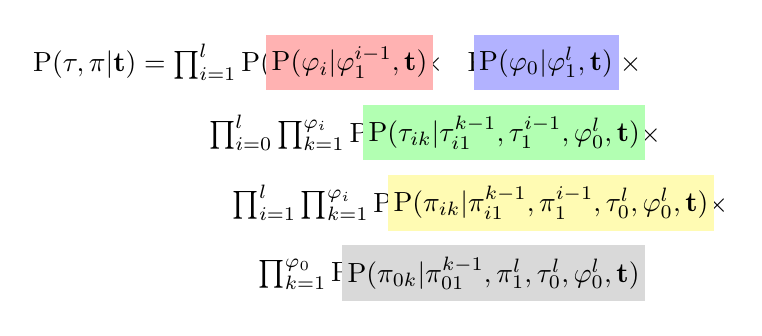
\begin{tikzpicture}



\node [anchor=west,inner sep=2pt,minimum height=2.5em] (eq1) at (0,0) {${\textrm{P}(\tau,\pi|\mathbf{t}) =  \prod_{i=1}^{l}{\textrm{P}(\varphi_i|\varphi_{1}^{i-1},\mathbf{t})} \ \ \times \ \ {\textrm{P}(\varphi_0|\varphi_{1}^{l},\mathbf{t})}\ \ \times}$};
\node [anchor=north west,inner sep=2pt,minimum height=2.5em] (eq2) at ([xshift=-16.06em,yshift=0.0em]eq1.south east) {${\prod_{i=0}^l{\prod_{k=1}^{\varphi_i}{\textrm{P}(\tau_{ik}|\tau_{i1}^{k-1},\tau_{1}^{i-1},\varphi_{0}^{l},\mathbf{t} )}} \ \ \times}$};
\node [anchor=north west,inner sep=2pt,minimum height=2.5em] (eq3) at ([xshift=-15.9em,yshift=0.0em]eq2.south east) {${\prod_{i=1}^l{\prod_{k=1}^{\varphi_i}{\textrm{P}(\pi_{ik}|\pi_{i1}^{k-1},\pi_{1}^{i-1},\tau_{0}^{l},\varphi_{0}^{l},\mathbf{t} )}} \ \ \times}$};
\node [anchor=north west,inner sep=2pt,minimum height=2.5em] (eq4) at ([xshift=-17.40em,yshift=0.0em]eq3.south east) {{${\prod_{k=1}^{\varphi_0}{\textrm{P}(\pi_{0k}|\pi_{01}^{k-1},\pi_{1}^{l},\tau_{0}^{l},\varphi_{0}^{l},\mathbf{t} )}}$}};

\node [anchor=west,inner sep=2pt,minimum height=2.0em,fill=red!30] (part1) at ([xshift=-13.8em,yshift=0.0em]eq1.east) {{${\textrm{P}(\varphi_i|\varphi_{1}^{i-1},\mathbf{t})}$}};
\node [anchor=west,inner sep=2pt,minimum height=2.0em,fill=blue!30] (part2) at ([xshift=-6.3em,yshift=0.0em]eq1.east) {{${\textrm{P}(\varphi_0|\varphi_{1}^{l},\mathbf{t})}$}};
\node [anchor=west,inner sep=2pt,minimum height=2.0em,fill=green!30] (part3) at ([xshift=-11em,yshift=0.0em]eq2.east) {{${\textrm{P}(\tau_{ik}|\tau_{i1}^{k-1},\tau_{1}^{i-1},\varphi_{0}^{l},\mathbf{t} )}$}};
\node [anchor=west,inner sep=2pt,minimum height=2.0em,fill=yellow!30] (part4) at ([xshift=-12.53em,yshift=0.0em]eq3.east) {{${\textrm{P}(\pi_{ik}|\pi_{i1}^{k-1},\pi_{1}^{i-1},\tau_{0}^{l},\varphi_{0}^{l},\mathbf{t} )}$}};
\node [anchor=west,inner sep=2pt,minimum height=2.0em,fill=gray!30] (part5) at ([xshift=-10.4em,yshift=0.0em]eq4.east) {{${\textrm{P}(\pi_{0k}|\pi_{01}^{k-1},\pi_{1}^{l},\tau_{0}^{l},\varphi_{0}^{l},\mathbf{t} )}$}};


\end{tikzpicture}





   \caption{{$\textrm{P}(\tau,\pi|t)$}的详细表达式}
   \label{fig:3-31}
\end{figure}
%----------------------------------------------

%----------------------------------------------------------------------------------------
%    NEW SUB-SECTION
%----------------------------------------------------------------------------------------

\subsection{IBM 模型3}

\parinterval IBM模型3通过一些假设对图\ref{fig:3-31}所表示的基本模型进行了化简。具体来说,对于每个$i\in[1,l]$,假设$\textrm{P}(\varphi_i |\varphi_1^{i-1},\mathbf{t})$仅依赖于$\varphi_i$和$t_i$,$\textrm{P}(\pi_{ik}|\pi_{i1}^{k-1},\pi_1^{i-1},\tau_0^l,\varphi_0^l,\mathbf{t})$仅依赖于$\pi_{ik}$、$i$、$m$和$l$。而对于所有的$i\in[0,l]$,假设$\textrm{P}(\tau_{ik}|\tau_{i1}^{k-1},\tau_1^{i-1},\phi_0^l,\mathbf{t})$仅依赖于$\tau_{ik}$和$t_i$。形式化这些假设,可以得到:
\begin{eqnarray}
\textrm{P}(\varphi_i|\varphi_1^{i-1},\mathbf{t})                                                              & = &{\textrm{P}(\varphi_i|t_i)} \label{eq:3-67} \\
\textrm{P}(\tau_{ik} = s_j |\tau_{i1}^{k-1},\tau_{1}^{i-1},\varphi_0^t,\mathbf{t})             & = & t(s_j|t_i) \label{eq:3-68} \\
\textrm{P}(\pi_{ik} = j |\pi_{i1}^{k-1},\pi_{1}^{i-1},\tau_{0}^{l},\varphi_{0}^{l},\mathbf{t}) & = & d(j|i,m,l) \label{eq:3-69}
\label{eq:3-49}
\end{eqnarray}

\parinterval 通常把$d(j|i,m,l)$称为扭曲度函数。这里$\textrm{P}(\varphi_i|\varphi_1^{i-1},\mathbf{t})={\textrm{P}(\varphi_i|t_i)}$和${\textrm{P}(\pi_{ik}=j|\pi_{i1}^{k-1},}$ $\pi_{1}^{i-1},\tau_0^l,\varphi_0^l,\mathbf{t})=d(j|i,m,l)$仅对$1 \le i \le l$成立。这样就完成了图\ref{fig:3-31}中第1、 3和4部分的建模。

\parinterval 对于$i=0$的情况需要单独进行考虑。实际上,$t_0$只是一个虚拟的单词。它要对应$\mathbf{s}$中原本为空对齐的单词。这里假设要等其他非空对应单词都被生成(放置)后,才考虑这些空对齐单词的生成(放置)。即非空对单词都被生成后,在那些还有空的位置上放置这些空对的源语单词。此外,在任何的空位置上放置空对的源语单词都是等概率的,即放置空对齐源语言单词服从均匀分布。这样在已经放置了$k$个空对齐源语言单词的时候,应该还有$\varphi_0-k$个空位置。如果第$i$个位置为空,那么$\textrm{P}(\pi_{0k}=i|\pi_{01}^{k-1},\pi_1^l,\tau_0^l,\varphi_0^l,\mathbf{t})=\frac{1}{\varphi_0-k}$,否则$\textrm{P}(\pi_{0k}=i|\pi_{01}^{k-1},\pi_1^l,\tau_0^l,\varphi_0^l,\mathbf{t})=0$。这样对于$t_0$所对应的$\tau_0$,就有
{
\begin{eqnarray}
\prod_{k=1}^{\varphi_0}{\textrm{P}(\pi_{0k}|\pi_{01}^{k-1},\pi_{1}^{l},\tau_{0}^{l},\varphi_{0}^{l},\mathbf{t})         }=\frac{1}{\varphi_{0}!}
\label{eq:3-50}
\end{eqnarray}
}
\parinterval 而上面提到的$t_0$所对应的这些空位置是如何生成的呢?即如何确定哪些位置是要放置空对齐的源语言单词。在IBM模型3中,假设在所有的非空对齐源语言单词都被生成出来后(共$\varphi_1+\varphi_2+\cdots {\varphi}_l$个非空对源语单词),这些单词后面都以$p_1$概率随机地产生一个``槽''用来放置空对齐单词。这样,${\varphi}_0$就服从了一个二项分布。于是得到
{
\begin{eqnarray}
\textrm{P}(\varphi_0|\mathbf{t})=\big(\begin{array}{c}
\varphi_1+\varphi_2+\cdots \varphi_l\\
\varphi_0\\
\end{array}\big)p_0^{\varphi_1+\varphi_2+\cdots \varphi_l-\varphi_0}p_1^{\varphi_0}
\label{eq:3-51}
\end{eqnarray}
}
\noindent 其中,$p_0+p_1=1$。到此为止,我们完成了图\ref{fig:3-31}中第2和5部分的建模。最终根据这些假设可以得到$\textrm{P}(\mathbf{s}| \mathbf{t})$的形式:
{
\begin{eqnarray}
{\textrm{P}(\mathbf{s}| \mathbf{t})}&= &{\sum_{a_1=0}^{l}{\cdots}\sum_{a_m=0}^{l}{\Big[\big(\begin{array}{c}
m-\varphi_0\\
\varphi_0\\
\end{array}\big)}p_0^{m-2\varphi_0}p_1^{\varphi_0}\prod_{i=1}^{l}{{\varphi_i}!n(\varphi_i|t_i)    }} \nonumber \\
& & \times{\prod_{j=1}^{m}{t(s_j|t_{a_j})} \times \prod_{j=1,a_j\neq 0}^{m}{d(j|a_j,m,l)}} \Big]
\label{eq:3-52}
\end{eqnarray}
}
\noindent 其中,$n(\varphi_i |t_i)={\textrm{P}(\varphi_i|t_i)}$表示产出率的分布。这里的约束条件为,
{
\begin{eqnarray}
\sum_{s}t(s|t)                     & = &1 \label{eq:3-53} \\
\sum_{j}d(j|i,m,l)                & = & 1 \label{eq:3-54} \\
\sum_{\varphi} n(\varphi|t) & = &1 \label{eq:3-55} \\
p_0+p_1                            & = & 1 \label{eq:3-56}
\end{eqnarray}
}

%----------------------------------------------------------------------------------------
%    NEW SUB-SECTION
%----------------------------------------------------------------------------------------
\vspace{-2em}
\subsection{IBM 模型4}

\parinterval IBM模型3仍然存在问题,比如,它不能很好地处理一个目标语言单词生成多个源语言单词的情况。这个问题在模型1和模型2中也存在。如果一个目标语言单词对应多个源语言单词,往往这些源语言单词构成短语或搭配。但是模型1-3把这些源语言单词看成独立的单元,而实际上它们是一个整体。这就造成了在模型1-3中这些源语言单词可能会``分散''开。为了解决这个问题,模型4对模型3进行了进一步修正。

\parinterval 为了更清楚的阐述,这里引入新的术语\ \dash \ {\small\bfnew{概念单元}}\index{概念单元}或{\small\bfnew{概念}}\index{概念}(Concept)\index{Concept}。词对齐可以被看作概念之间的对应。这里的概念是指具有独立语法或语义功能的一组单词。依照Brown等人的表示方法\cite{Peter1993The},可以把概念记为cept.。每个句子都可以被表示成一系列的cept.。这里要注意的是,源语言句子中的cept.数量不一定等于目标句子中的cept.数量。因为有些cept. 可以为空,因此可以把那些空对的单词看作空cept.。比如,在图\ref{fig:3-32}的实例中,``了''就对应一个空cept.。
\vspace{3em}

%----------------------------------------------
\begin{figure}[htp]
    \centering
%%% outline
%-------------------------------------------------------------------------
\begin{tikzpicture}

{
{\footnotesize
\node [anchor=north west,minimum height=2em,minimum width=4em] (s11) at (0,0) {};
\node [rectangle,draw,anchor=west,line width=1pt,minimum height=2em,minimum width=4em,fill=green!30,drop shadow] (s1) at ([xshift=2em]s11.east) {我};
\node [rectangle,draw,anchor=west,line width=1pt,minimum height=2em,minimum width=4em,fill=green!30,drop shadow] (s2) at ([xshift=2em]s1.east) {改变};
\node [rectangle,draw,anchor=west,line width=1pt,minimum height=2em,minimum width=4em,fill=green!30,drop shadow] (s3) at ([xshift=2em]s2.east) {主意};
\node [rectangle,draw,anchor=west,line width=1pt,minimum height=2em,minimum width=4em,fill=green!30,drop shadow] (s4) at ([xshift=2em]s3.east) {了};
\node [rectangle,draw,anchor=west,line width=1pt,minimum height=2em,minimum width=4em,fill=green!30,drop shadow] (s5) at ([xshift=2em]s4.east) {。};

\node [anchor=south] (nu1) at (s1.north) {1};
\node [anchor=south] (nu2) at (s2.north) {2};
\node [anchor=south] (nu3) at (s3.north) {3};
\node [anchor=south] (nu4) at (s4.north) {4};
\node [anchor=south] (nu5) at (s5.north) {5};
}

{
{\footnotesize
\node [anchor=north,rectangle,draw,line width=1pt,minimum height=2em,minimum width=4em,fill=red!30,drop shadow] (t1) at ([yshift=-3.5em]s11.south) {$t_0$};
\node [rectangle,draw,anchor=north,line width=1pt,minimum height=2em,minimum width=4em,fill=red!30,drop shadow] (t2) at ([yshift=-3.5em]s1.south) {I};
\node [rectangle,draw,anchor=north,line width=1pt,minimum height=2em,minimum width=4em,fill=red!30,drop shadow] (t3) at ([yshift=-3.5em]s2.south) {changed};
\node [rectangle,draw,anchor=north,line width=1pt,minimum height=2em,minimum width=4em,fill=red!30,drop shadow] (t4) at ([yshift=-3.5em]s3.south) {my};
\node [rectangle,draw,anchor=north,line width=1pt,minimum height=2em,minimum width=4em,fill=red!30,drop shadow] (t5) at ([yshift=-3.5em]s4.south) {mind};
\node [rectangle,draw,anchor=north,line width=1pt,minimum height=2em,minimum width=4em,fill=red!30,drop shadow] (t6) at ([yshift=-3.5em]s5.south) {.};

\node [anchor=north] (nd1) at (t2.south) {[1]};
\node [anchor=north] (nd2) at (t3.south) {[2]};
\node [anchor=north] (nd3) at (t5.south) {[3]};
\node [anchor=north] (nd4) at (t6.south) {[4]};
}
\draw [->,thick] (s1.south) -- (t2.north);
\draw [->,thick] (s2.south) -- (t3.north);
\draw [->,thick] (s3.south) -- (t5.north);
\draw [->,thick] (s4.south) -- (t1.north);
\draw [->,thick] (s5.south) -- (t6.north);
}

\node [anchor=east] (ss) at ([xshift=-0.5em]s1.west) {$\seq{s}$};
\node [anchor=east] (tt) at ([xshift=-0.5em]t1.west) {$\seq{t}$};

}
\end{tikzpicture}
%---------------------------------------------------------------------
   \caption{词对齐的汉译英句对及独立单词cept.的位置}
   \label{fig:3-32}
\end{figure}
%----------------------------------------------

\parinterval 在IBM模型的词对齐框架下,目标语的cept.只能是那些非空对齐的目标语单词,而且每个cept.只能由一个目标语单词组成(通常把这类由一个单词组成的cept.称为独立单词cept.)。这里用$[i]$表示第$i$ 个独立单词cept.在目标语言句子中的位置。换句话说,$[i]$表示第$i$个非空对的目标语单词的位置。比如在本例中``mind''在$\mathbf{t}$中的位置表示为$[3]$。

\parinterval 另外,可以用$\odot_{i}$表示位置为$[i]$的目标语言单词对应的那些源语言单词位置的平均值,如果这个平均值不是整数则对它向上取整。比如在本例中,目标语句中第4个cept. (``.'')对应在源语言句子中的第5个输出值。可表示为${\odot}_{4}=5$。

\parinterval 利用这些新引进的概念,模型4对模型3的扭曲度进行了修改。主要是把扭曲度分解为两类参数。对于$[i]$对应的源语言单词列表($\tau_{[i]}$)中的第一个单词($\tau_{[i]1}$),它的扭曲度用如下公式计算:
\begin{equation}
\textrm{P}(\pi_{[i]1}=j|{\pi}_1^{[i]-1},{\tau}_0^l,{\varphi}_0^l,\mathbf{t})=d_{1}(j-{\odot}_{i-1}|A(t_{[i-1]}),B(s_j))
\label{eq:3-70}
\end{equation}

\noindent 其中,译文的第$i$个单词生成的第$k$个源语单词在源语言句子中的位置用变量$\pi_{ik}$表示。而对于列表($\tau_{[i]}$)中的其他的单词($\tau_{[i]k},1 < k \le \varphi[i]$)的扭曲度计算,进行如下计算
\begin{equation}
\textrm{P}(\pi_{[i]k}=j|{\pi}_{[i]1}^{k-1},\pi_1^{[i]-1},\tau_0^l,\varphi_0^l,\mathbf{t})=d_{>1}(j-\pi_{[i]k-1}|B(s_j))
\label{eq:3-71}
\end{equation}

\parinterval 这里的函数$A(\cdot)$和函数$B(\cdot)$分别把目标语言和源语言的单词影射到单词的词类。这么做的目的一方面要减小参数空间的大小,另一方面是要减小数据的稀疏程度。词类信息通常可以通过外部工具得到,比如Brown聚类等。另一种简单的方法是把单词直接映射为它的词性。这样可以直接用现在已经非常成熟的词性标注工具解决问题。

\parinterval 从上面改进的扭曲度模型可以看出,对于$t_{[i]}$生成的第一个源语言单词,要考虑中心$\odot_{[i]}$和这个源语言单词之间的绝对距离。实际上也就要把$t_{[i]}$生成的所有源语言单词看成一个整体并把它放置在合适的位置。这个过程要依据第一个源语言单词的词类和对应源语中心位置,和前一个非空对目标语言单词$t_{[i-1]}$的词类。而对于$t[i]$生成的其他源语言单词,只需要考虑它与前一个刚放置完的源语言单词的相对位置和这个源语言单词的词类。

\parinterval 实际上,上述过程就要先用$t_{[i]}$生成的第一个源语言单词代表整个$t_{[i]}$生成的单词列表,并把第一个源语言单词放置在合适的位置。然后,相对于前一个刚生成的源语言单词,把列表中的其他单词放置在合适的地方。这样就可以在一定程度上保证由同一个目标语言单词生成的源语言单词之间可以相互影响,达到了改进的目的。

%----------------------------------------------------------------------------------------
%    NEW SUB-SECTION
%----------------------------------------------------------------------------------------

\subsection{ IBM 模型5}

\parinterval 模型3和模型4并不是``准确''的模型。这两个模型会把一部分概率分配给一些根本就不存在的句子。这个问题被称作IBM模型3和模型4的{\small\bfnew{缺陷}}\index{缺陷}(Deficiency)\index{Deficiency}。说的具体一些,模型3和模型4 中并没有这样的约束:如果已经放置了某个源语言单词的位置不能再放置其他单词,也就是说句子的任何位置只能放置一个词,不能多也不能少。由于缺乏这个约束,模型3和模型4中在所有合法的词对齐上概率和不等于1。 这部分缺失的概率被分配到其他不合法的词对齐上。举例来说,如图\ref{fig:3-33}所示,``吃 早饭''和``have breakfast''之间的合法词对齐用直线表示 。但是在模型3和模型4中, 在它们上的概率和为$0.9<1$。 损失掉的概率被分配到像5和6这样的对齐上了(红色)。虽然IBM模型并不支持一对多的对齐,但是模型3和模型4把概率分配给这些``不合法''的词对齐上,因此也就产生所谓的Deficiency问题。

%----------------------------------------------
\begin{figure}[htp]
    \centering


%%% outline
%-------------------------------------------------------------------------


%%% 简易机器翻译系统 - step 3 decoding - example


\begin{tikzpicture}


\begin{scope}[scale=0.6]
\node [anchor=west] (eq1) at (0,0) {吃};
\node [anchor=west] (eq2) at ([xshift=3.0em,yshift=0.0em]eq1.east) {早饭};
\node [anchor=north] (eq3) at ([xshift=0.0em,yshift=-2.0em]eq1.south) {have};
\node [anchor=north] (eq4) at ([xshift=0.0em,yshift=-2.0em]eq2.south) {breakfast};
\node [anchor=east] (eq5) at ([xshift=-1.0em,yshift=-1.8em]eq1.west) {$\mathbf{a}_{1}$};
\node [anchor=west] (eq6) at ([xshift=1.0em,yshift=-1.8em]eq2.east) {$\textrm{P}(\mathbf{s},\mathbf{a}_{1}|\mathbf{t})=0.5$};
\draw [-,very thick](eq1.south) -- (eq3.north);
\draw [-,very thick](eq2.south) -- (eq4.north);
\node [anchor=west] (eq7) at ([xshift=13.1em,yshift=1.4em]eq2.east) {};
\node [anchor=west] (eq8) at ([xshift=13.1em,yshift=-25.6em]eq2.east) {};
\node [anchor=south] (eq9) at ([xshift=0.0em,yshift=0.0em]eq7.north) {吃早饭 $\Leftrightarrow $ have breakfast};


\draw [-,very thick,dotted](eq7.south) -- (eq8.north);


\end{scope}

\begin{scope}[scale=0.6,xshift=0.0,yshift=-10.0em]
\node [anchor=west] (eq1) at (0,0) {吃};
\node [anchor=west] (eq2) at ([xshift=3.0em,yshift=0.0em]eq1.east) {早饭};
\node [anchor=north] (eq3) at ([xshift=0.0em,yshift=-2.0em]eq1.south) {have};
\node [anchor=north] (eq4) at ([xshift=0.0em,yshift=-2.0em]eq2.south) {breakfast};
\node [anchor=east] (eq5) at ([xshift=-1.0em,yshift=-1.8em]eq1.west) {$\mathbf{a}_{2}$};
\node [anchor=west] (eq6) at ([xshift=1.0em,yshift=-1.8em]eq2.east) {$\textrm{P}(\mathbf{s},\mathbf{a}_{2}|\mathbf{t})=0.1$};
\draw [-,very thick](eq1.south) -- (eq4.north);
\draw [-,very thick](eq2.south) -- (eq3.north);
\end{scope}

\begin{scope}[scale=0.6,xshift=0.0,yshift=-20.0em]
\node [anchor=west] (eq1) at (0,0) {吃};
\node [anchor=west] (eq2) at ([xshift=3.0em,yshift=0.0em]eq1.east) {早饭};
\node [anchor=north] (eq3) at ([xshift=0.0em,yshift=-2.0em]eq1.south) {have};
\node [anchor=north] (eq4) at ([xshift=0.0em,yshift=-2.0em]eq2.south) {breakfast};
\node [anchor=east] (eq5) at ([xshift=-1.0em,yshift=-1.8em]eq1.west) {$\mathbf{a}_{3}$};
\node [anchor=west] (eq6) at ([xshift=1.0em,yshift=-1.8em]eq2.east) {$\textrm{P}(\mathbf{s},\mathbf{a}_{3}|\mathbf{t})=0.1$};
\draw [-,very thick](eq1.south) -- (eq3.north);
\draw [-,very thick](eq2.south) -- (eq3.north);
\end{scope}

\begin{scope}[scale=0.6,xshift=29.0em,yshift=0.0em]
\node [anchor=west] (eq1) at (0,0) {吃};
\node [anchor=west] (eq2) at ([xshift=3.0em,yshift=0.0em]eq1.east) {早饭};
\node [anchor=north] (eq3) at ([xshift=0.0em,yshift=-2.0em]eq1.south) {have};
\node [anchor=north] (eq4) at ([xshift=0.0em,yshift=-2.0em]eq2.south) {breakfast};
\node [anchor=east] (eq5) at ([xshift=-1.0em,yshift=-1.8em]eq1.west) {$\mathbf{a}_{4}$};
\node [anchor=west] (eq6) at ([xshift=1.0em,yshift=-1.8em]eq2.east) {$\textrm{P}(\mathbf{s},\mathbf{a}_{4}|\mathbf{t})=0.1$};
\draw [-,very thick](eq1.south) -- (eq4.north);
\draw [-,very thick](eq2.south) -- (eq4.north);
\end{scope}

\begin{scope}[scale=0.6,xshift=29.0em,yshift=-10.0em]
\node [anchor=west] (eq1) at (0,0) {吃};
\node [anchor=west] (eq2) at ([xshift=3.0em,yshift=0.0em]eq1.east) {早饭};
\node [anchor=north] (eq3) at ([xshift=0.0em,yshift=-2.0em]eq1.south) {have};
\node [anchor=north] (eq4) at ([xshift=0.0em,yshift=-2.0em]eq2.south) {breakfast};
\node [anchor=east] (eq5) at ([xshift=-1.0em,yshift=-1.8em]eq1.west) {$\mathbf{a}_{5}$};
\node [anchor=west] (eq6) at ([xshift=1.0em,yshift=-1.8em]eq2.east) {$\textrm{P}(\mathbf{s},\mathbf{a}_{5}|\mathbf{t})=0.05$};
\draw [-,very thick](eq1.south) -- (eq3.north);
\draw [-,very thick](eq1.south) -- (eq4.north);
\draw [-,very thick](eq2.south) -- (eq3.north);
\node [anchor=west,very thick,draw=red,minimum width=1.5em,minimum height=1.5em] (w1) at (eq5.west){};
\node [anchor=west,very thick,draw=red,minimum width=7.7em,minimum height=1.5em] (w2) at (eq6.west){};

\end{scope}

\begin{scope}[scale=0.6,xshift=29.0em,yshift=-20.0em]
\node [anchor=west] (eq1) at (0,0) {吃};
\node [anchor=west] (eq2) at ([xshift=3.0em,yshift=0.0em]eq1.east) {早饭};
\node [anchor=north] (eq3) at ([xshift=0.0em,yshift=-2.0em]eq1.south) {have};
\node [anchor=north] (eq4) at ([xshift=0.0em,yshift=-2.0em]eq2.south) {breakfast};
\node [anchor=east] (eq5) at ([xshift=-1.0em,yshift=-1.8em]eq1.west) {$\mathbf{a}_{6}$};
\node [anchor=west] (eq6) at ([xshift=1.0em,yshift=-1.8em]eq2.east) {$\textrm{P}(\mathbf{s},\mathbf{a}_{6}|\mathbf{t})=0.05$};
\draw [-,very thick](eq1.south) -- (eq3.north);
\draw [-,very thick](eq2.south) -- (eq4.north);
\draw [-,very thick](eq2.south) -- (eq3.north);
\node [anchor=west,very thick,draw=red,minimum width=1.5em,minimum height=1.5em] (w1) at (eq5.west){};
\node [anchor=west,very thick,draw=red,minimum width=7.7em,minimum height=1.5em] (w2) at (eq6.west){};
\end{scope}




\end{tikzpicture}





    \caption{IBM模型3的词对齐及概率分配}
    \label{fig:3-33}
\end{figure}
%----------------------------------------------

\parinterval 为了解决这个问题,模型5在模型中增加了额外的约束。基本想法是,在放置一个源语言单词的时候检查这个位置是否已经放置了单词,如果可以则把这个放置过程赋予一定的概率,否则把它作为不可能事件。依据这个想法,就需要在逐个放置源语言单词的时候判断源语言句子的哪些位置为空。这里引入一个变量$v(j, {\tau_1}^{[i]-1}, \tau_{[i]1}^{k-1})$,它表示在放置$\tau_{[i]k}$之前($\tau_1^{[i]-1}$和$\tau_{[i]1}^{k-1}$已经被放置完了),从源语言句子的第一个位置到位置$j$(包含$j$)为止还有多少个空位置。这里,把这个变量简写为$v_j$。于是,对于$[i]$所对应的源语言单词列表($\tau_{[i]}$)中的第一个单词($\tau_{[i]1}$),有:
\begin{eqnarray}
\textrm{P}(\pi_{[i]1} = j | \pi_1^{[i]-1}, \tau_0^l, \varphi_0^l, \mathbf{t}) & = & d_1(v_j|B(s_j), v_{\odot_{i-1}}, v_m-(\varphi_{[i]}-1)) \cdot \nonumber \\
                                                                                                   &     & (1-\delta(v_j,v_{j-1}))
\label{eq:3-57}
\end{eqnarray}

\parinterval 对于其他单词($\tau_{[i]k}$, $1 < k\le\varphi_{[i]}$),有:
\begin{eqnarray}
&   & \textrm{P}(\pi_{[i]k}=j|\pi_{[i]1}^{k-1}, \pi_1^{[i]-1}, \tau_0^l, \varphi_0^l,\mathbf{t}) \nonumber \\
&= & d_{>1}(v_j-v_{\pi_{[i]k-1}}|B(s_j), v_m-v_{\pi_{[i]k-1}}-\varphi_{[i]}+k) \cdot (1-\delta(v_j,v_{j-1}))
\label{eq:3-58}
\end{eqnarray}

\noindent 这里,因子$1-\delta(v_i, v_{i-1})$是用来判断第$i$个位置是不是为空。如果第$i$个位置为空则$v_i = v_{i-1}$,这样$\textrm{P}(\pi_{[i]1}=i|\pi_1^{[i]-1}, \tau_0^l, \varphi_0^l, \mathbf{t}) = 0$。这样就从模型上避免了模型3和模型4中生成不存在的字符串的问题。这里还要注意的是,对于放置第一个单词的情况,影响放置的因素有$v_i$,$B(s_i)$和$v_{i-1}$。此外还要考虑在$i$位置放置了第一个单词以后它的右边是不是还有足够的位置留给剩下的$k-1$个单词。参数$v_m-(\varphi_{[i]}-1)$正是为了考虑这个因素,这里$v_m$表示整个源语言句子中还有多少空位置,$\varphi_{[i]}-1$表示$i$位置右边至少还要留出的空格数。对于放置非第一个单词的情况,主要是要考虑它和前一个放置位置的相对位置。这主要体现在参数$v_i-v_{\varphi_{[i]}k-1}$上。式\ref{eq:3-58}的其他部分都可以用上面的理论解释,这里不再赘述。

\parinterval 实际上,模型5和模型4的思想基本一致,即,先确定$\tau_{[i]1}$的绝对位置,然后再确定$\tau_{[i]}$中剩余单词的相对位置。模型5消除了产生不存在的句子的可能性,不过模型5的复杂性也大大增加了。

%----------------------------------------------------------------------------------------
%    NEW SUB-SECTION
%----------------------------------------------------------------------------------------

\subsection{隐马尔可夫模型}

\parinterval IBM模型可以得到双语句子间的词对齐,因此也有很多工作在这个模型的基础上对词对齐方法进行改进。其中一个比较有代表性的工作是基于隐马尔可夫模型的方法\cite{vogel1996hmm},它可以被看作是IBM 模型2的升级版本。

%----------------------------------------------------------------------------------------
%    NEW SUBSUB-SECTION
%----------------------------------------------------------------------------------------

\subsubsection{隐马尔可夫模型}

\parinterval {\small\sffamily\bfseries{隐马尔可夫模型}}(Hidden Markov Model,HMM)是经典的机器学习模型,它在语音识别、自然语言处理等领域得到了非常广泛的应用。其本质是一个概率模型,用来描述一个含有隐含参数的马尔可夫过程,简单来说,是用来描述一个系统,它隐含状态的转移和可见状态的概率\footnote{https://zh.wikipedia.org/zh-hans/隐马尔可夫模型}。

\parinterval 我们用一个简单的例子来对这些概念进行说明。假设有三枚质地不同的硬币A、B、C,这三个硬币抛出正面的概率分别为0.3、0.5、0.7。之后开始抛硬币,随机从三个硬币里挑一个,挑到每一个硬币的概率都是$1/3$。不停的重复上述过程,会得到一串硬币的正反序列,如:抛硬币6次,得到:正 正 反 反 正 反。

\parinterval 这个正反序列叫做可见状态链,由每个回合的可见状态构成。此外,HMM模型还有一串隐含状态链,在这里,隐含状态链就是所用硬币的序列,比如可能是:C B A B C A。同样的,HMM模型还会描述系统隐藏状态的转移概率,在本例子中,A的下一个状态是A、B、C的概率都是$1/3$。B、C的下一个状态是A、B、C的转移概率也同样是$1/3$。同样的,尽管可见状态链之间没有转移概率,但是隐含状态和可见状态之间存在着输出概率,即A、B、C抛出正面的输出概率为0.3、0.5、0.7。图\ref{fig:3-34}描述了这个例子所对应的的隐马尔可夫模型示意图。

%----------------------------------------------
\begin{figure}[htp]
    \centering

\definecolor{ublue}{rgb}{0.152,0.250,0.545}
\definecolor{ugreen}{rgb}{0,0.5,0}



%%% outline
%-------------------------------------------------------------------------


%%% 简易机器翻译系统 - step 3 decoding - example


\begin{tikzpicture}


\begin{scope}[scale=0.4]
{\footnotesize
\node [anchor=west,draw,thick,minimum width=2.8em, minimum height=2.0em,fill=green!30,drop shadow](num1) at (0,0) {C};
\node [anchor=north,circle,draw,thick,minimum width=2.0em,fill=red!30,drop shadow](num1-1) at ([yshift=-5.0em]num1.south) {正};
\draw [->,very thick,ublue]([yshift=-0.2em]num1.south) -- ([yshift=0.2em]num1-1.north);

%%%%%%%%%%%%%%%%%%%%%%%%%%
\node [anchor=west,draw,thick,minimum width=2.8em, minimum height=2.0em,fill=green!30,drop shadow](num2) at ([xshift=5.2em]num1.east)  {B};
\node [anchor=north,circle,draw,thick,minimum width=2.0em,fill=red!30,drop shadow](num2-1) at ([yshift=-5.0em]num2.south) {正};
\draw [->,very thick]([xshift=0.2em]num1.east) -- ([xshift=-0.2em]num2.west);
\draw [->,very thick,ublue]([yshift=-0.2em]num2.south) -- ([yshift=0.2em]num2-1.north);

%%%%%%%%%%%%%%%%%%%%%%%%%%
\node [anchor=west,draw,thick,minimum width=2.8em, minimum height=2.0em,fill=green!30,drop shadow](num3) at ([xshift=5.2em]num2.east)  {A};
\node [anchor=north,circle,draw,thick,minimum width=2.0em,fill=red!30,drop shadow](num3-1) at ([yshift=-5.0em]num3.south) {反};
\draw [->,very thick]([xshift=0.2em]num2.east) -- ([xshift=-0.2em]num3.west);
\draw [->,very thick,ublue]([yshift=-0.2em]num3.south) -- ([yshift=0.2em]num3-1.north);

%%%%%%%%%%%%%%%%%%%%%%%%%%
\node [anchor=west,draw,thick,minimum width=2.8em, minimum height=2.0em,fill=green!30,drop shadow](num4) at ([xshift=5.2em]num3.east)  {B};
\node [anchor=north,circle,draw,thick,minimum width=2.0em,fill=red!30,drop shadow](num4-1) at ([yshift=-5.0em]num4.south) {反};
\draw [->,very thick]([xshift=0.2em]num3.east) -- ([xshift=-0.2em]num4.west);
\draw [->,very thick,ublue]([yshift=-0.2em]num4.south) -- ([yshift=0.2em]num4-1.north);

%%%%%%%%%%%%%%%%%%%%%%%%%%
\node [anchor=west,draw,thick,minimum width=2.8em, minimum height=2.0em,fill=green!30,drop shadow](num5) at ([xshift=5.2em]num4.east)  {C};
\node [anchor=north,circle,draw,thick,minimum width=2.0em,fill=red!30,drop shadow](num5-1) at ([yshift=-5.0em]num5.south) {正};
\draw [->,very thick]([xshift=0.2em]num4.east) -- ([xshift=-0.2em]num5.west);
\draw [->,very thick,ublue]([yshift=-0.2em]num5.south) -- ([yshift=0.2em]num5-1.north);

%%%%%%%%%%%%%%%%%%%%%%%%%%
\node [anchor=west,draw,thick,minimum width=2.8em, minimum height=2.0em,fill=green!30,drop shadow](num6) at ([xshift=5.2em]num5.east)  {A};
\node [anchor=north,circle,draw,thick,minimum width=2.0em,fill=red!30,drop shadow](num6-1) at ([yshift=-5.0em]num6.south) {反};
\draw [->,very thick]([xshift=0.2em]num5.east) -- ([xshift=-0.2em]num6.west);
\draw [->,very thick,ublue]([yshift=-0.2em]num6.south) -- ([yshift=0.2em]num6-1.north);

\node [anchor=north](word1) at ([xshift=2.5em,yshift=-3.0em]num1-1.south)  {图示说明:};
\node [anchor=north,draw,thick,minimum width=2.8em, minimum height=2.0em,fill=green!30,drop shadow](word2) at ([xshift=-2.5em,yshift=-3.0em]word1.south)  {C};
\node [anchor=west](word2-2) at ([xshift=1.5em]word2.east)  {一个隐含状态};
\node [anchor=north,circle,draw,thick,minimum width=2.0em,fill=red!30,drop shadow](word3) at ([xshift=-2.5em,yshift=-12.2em]word1.south) {正};
\node [anchor=west](word3-2) at ([xshift=2.1em]word3.east)  {一个可见状态};

\draw [->,very thick]([xshift=6.4em]word2-2.east) -- ([xshift=11.6em]word2-2.east);
\node [anchor=west](word4) at ([xshift=13.1em]word2-2.east)  {从一个隐含状态到下一个};
\node [anchor=west](word4-1) at ([xshift=13.1em,yshift=-4.0em]word2-2.east)  {隐含状态的转换};

\draw [->,very thick,ublue]([xshift=30.7em,yshift=-0.2em]word3.north) -- ([xshift=30.7em,yshift=0.2em]word3.south);

\node [anchor=west](word5) at ([xshift=13.1em,yshift=-9.5em]word2-2.east)  {从一个隐含状态到可见状};
\node [anchor=west](word5-1) at ([xshift=13.1em,yshift=-13.5em]word2-2.east)  {态的输出};
}
\end{scope}

\end{tikzpicture}

























    \caption{抛硬币的隐马尔可夫模型实例}
    \label{fig:3-34}
\end{figure}
%----------------------------------------------

\parinterval 一般来说,HMM包含下面三个问题\cite{manning1999foundations}:

\begin{itemize}
\vspace{0.5em}
\item 估计:即给定模型(硬币种类和转移概率),根据可见状态链(抛硬币的结果),计算在该模型下得到这个结果的概率,这个问题的解决需要用到前后向算法。
\vspace{0.5em}
\item 参数学习:即给定硬币种类(隐含状态数量),根据多个可见状态链(抛硬币的结果),估计模型的参数(转移概率),同IBM模型的参数训练一样,这个问题的求解需要用到EM算法。
\vspace{0.5em}
\item 解码问题:即给定模型(硬币种类和转移概率)和可见状态链(抛硬币的结果),计算在可见状态链的情况下,最可能出现的对应的状态序列,这个问题的求解需要用到基于动态规划方法,在HMM中被称作维特比算法(Viterbi Algorithm)。
\vspace{0.5em}
\end{itemize}

%----------------------------------------------------------------------------------------
%    NEW SUBSUB-SECTION
%----------------------------------------------------------------------------------------
\vspace{-2em}
\subsubsection{词对齐模型}

\parinterval IBM模型把翻译问题定义为对译文和词对齐同时进行生成的问题,模型翻译质量的好坏与词对齐有着非常紧密的联系。IBM模型1假设对齐概率仅依赖于译文长度,即对齐概率服从均匀分布;IBM模型2假设对齐概率与源语言、目标语言的句子长度以及源语言位置和目标语言位置相关。IBM模型2已经覆盖到了大部分的词对齐问题,但是该模型只考虑到了词语的绝对位置,并未考虑到相邻词语间的关系。图\ref{fig:3-35}展示了一个简单的实例,可以看到的是,汉语的每个词都被分配给了英语句子中的每一个单词,但是词语并不是任意分布在各个位置上的,而是倾向于生成簇。也就是说,如果源语言的两个词位置越近,它们的目标词在目标语言句子的位置也越近。

%----------------------------------------------
\begin{figure}[htp]
    \centering

%%% outline
%-------------------------------------------------------------------------


\begin{tikzpicture}

\begin{scope}
\node [anchor=west] (s1) at (0,0) {\small{$s_1$}:我};
\node [anchor=west] (s2) at ([xshift=0.5em]s1.east) {\small{$s_2$}:对};
\node [anchor=west] (s3) at ([xshift=0.5em]s2.east) {\small{$s_3$}:你};
\node [anchor=west] (s4) at ([xshift=0.5em]s3.east) {\small{$s_4$}:感到};
\node [anchor=west] (s5) at ([xshift=0.5em]s4.east) {\small{$s_5$}:满意};
\end{scope}

\begin{scope}[yshift=-3.5em]
\node [anchor=west] (t1) at (0.45em,0) {\small{$t_1$}:I};
\node [anchor=west] (t2) at ([xshift=1.0em,yshift=0.0em]t1.east) {\small{$t_2$}:am};
\node [anchor=west] (t3) at ([xshift=0.3em,yshift=0.0em]t2.east) {\small{$t_3$}:satisfied};
\node [anchor=west] (t4) at ([xshift=0.3em]t3.east) {\small{$t_4$}:with};
\node [anchor=west] (t5) at ([xshift=0.3em,yshift=-0.0em]t4.east) {\small{$t_5$}:you};
\end{scope}


\draw [-,thick,dashed] (s1.south) -- (t1.north);
\draw [-,thick,dashed] (s4.south) -- ([yshift=0.3em]t2.north);
\draw [-,thick,dashed] (s2.south) ..controls +(south:1em) and +(north:1em).. (t4.north);
\draw [-,thick,dashed] (s3.south) ..controls +(south:0.5em) and +(north:1.5em).. (t5.north);
\draw [-,thick,dashed] (s5.south) -- (t3.north);

\end{tikzpicture}


%---------------------------------------------------------------------




    \caption{汉译英句对及对齐}
    \label{fig:3-35}
\end{figure}
%----------------------------------------------

\parinterval 因此,基于HMM的词对齐模型抛弃了IBM模型1-2的绝对位置假设,将一阶隐马尔可夫模型用于单词对齐问题。HMM词对齐模型认为,词语与词语之间并不是毫无联系的,对齐概率应该取决于对齐位置的差异而不是本身词语所在的位置。具体来说,位置$j$的对齐概率$a_j$与前一个位置$j-1$的对齐位置$a_{j-1}$和译文长度$l$有关,形式化的表述为:
\begin{eqnarray}
\textrm{P}(a_{j}|a_{1}^{j-1},s_{1}^{j-1},m,\mathbf{t})=\textrm{P}(a_{j}|a_{j-1},l)
\label{eq:3-59}
\end{eqnarray}

\parinterval 这里用图\ref{fig:3-34}的例子对公式进行说明。在IBM模型1-2中,词语的对齐都是与单词所在的绝对位置有关。但在HMM词对齐模型中,``你''对齐到``you''被形式化为$\textrm{P}(a_{j}|a_{j-1},l)= P(5|4,5)$,意思是对于源文位置$3(j=3)$的词,如果它的目标译文是5个词,上一个对齐位置是$4(a_{2}=4)$,对齐到目标语译文位置$5(a_{j}=5)$的概率是多少?理想的情况下,通过$\textrm{P}(a_{j}|a_{j-1},l)$,``你''对齐到``you''应该得到更高的概率,并且由于源语词``对''和``你''距离很近,因此其对应的对齐位置``with''和``you''的距离也应该很近。

\parinterval 因此,把公式\ref{eq:3-22}和\ref{eq:3-59}重新带入公式1.19和1.18,可得HMM词对齐模型的数学描述:
\begin{eqnarray}
\textrm{P}(\mathbf{s}| \mathbf{t})=\sum_{\mathbf{a}}{\textrm{P}(m|\mathbf{t})}\prod_{j=1}^{m}{\textrm{P}(a_{j}|a_{j-1},l)f(s_{j}|t_{a_j})}
\label{eq:3-60}
\end{eqnarray}

\parinterval 此外,为了使得HMM的对齐概率$\textrm{P}(a_{j}|a_{j-1},l)$满足归一化的条件,这里还假设其对齐概率只取决于$a_{j}-a_{j-1}$,即:
\begin{eqnarray}
\textrm{P}(a_{j}|a_{j-1},l)=\frac{\mu(a_{j}-a_{j-1})}{\sum_{i=1}^{l}{\mu(i-a_{j-1})}}
\label{eq:3-61}
\end{eqnarray}

\noindent 其中,$\mu( \cdot )$是隐马尔可夫模型的参数,可以通过训练得到。

%----------------------------------------------------------------------------------------
%    NEW SUB-SECTION
%----------------------------------------------------------------------------------------

\subsection{解码和训练}

\parinterval 和IBM模型1-2一样,IBM模型3-5和隐马尔可夫模型的解码可以直接使用\ref{sec:sentence-level-translation}\\节所描述的方法。基本思路是对译文自左向右生成,每次扩展一个源语言单词的翻译,即把源语言单词的译文放到已经生成的译文的右侧。每次扩展可以选择不同的源语言单词或者同一个源语言单词的不同翻译候选,这样就可以得到多个不同的扩展译文。在这个过程中,同时计算翻译模型和语言模型的得分,对每个得到译文候选打分。最终,保留一个或者多个译文。这个过程重复执行直至所有源语言单词被翻译完。

\parinterval 类似的,IBM模型3-5和隐马尔可夫模型也都可以使用期望最大化(EM)方法进行模型训练。相关数学推导可参考附录\ref{appendix-B}的内容。通常,可以使用这些模型获得双语句子间的词对齐结果,比如著名的GIZA++工具。这时,往往会使用多个模型,把简单的模型训练后的参数作为初始值送给后面更加复杂的模型。比如,先用IBM模型1训练,之后把参数送给IBM模型2,再训练,之后把参数送给隐马尔可夫模型等。值得注意的是,并不是所有的模型使用EM算法都能找到全局最优解。特别是IBM模型3-5的训练中使用一些剪枝和近似的方法,优化的真实目标函数会更加复杂。不过,IBM模型1是一个{\small\bfnew{凸函数}}\index{凸函数}(Convex Function)\index{Convex function},因此理论上使用EM方法是能找到全局最优解的。更实际的好处是,IBM模型1训练的最终结果与参数的初始化过程无关。这也是为什么在使用IBM系列模型时,往往会使用IBM模型1作为起始模型的原因。

%----------------------------------------------------------------------------------------
%    NEW SECTION
%----------------------------------------------------------------------------------------

\sectionnewpage
\section{问题分析}

\parinterval IBM模型是一个时代的经典,但也留下了一些值得思考的问题。这一方面体现了科学技术发展需要一步步前行,而非简单的一蹴而就。另一方面也体现了机器翻译问题的困难程度。下面对IBM存在的问题进行分析,同时给出一些解决问题的思路,希望通过这些讨论可以使我们对机器翻译问题有更深层次的理解。

%----------------------------------------------------------------------------------------
%    NEW SUB-SECTION
%----------------------------------------------------------------------------------------

\subsection{词对齐及对称化}

\parinterval IBM的五个模型都是基于一个词对齐的假设\ \dash \ 一个源语言单词最多只能对齐到一个目标语言单词。这个约束大大化简了IBM模型的建模。最初,Brown等人提出这个假设可能是因为在法英翻译中一对多的对齐情况并不多见,这个假设带来的问题也不是那么严重。但是,在像汉英翻译这样的任务中,一个汉语单词对应多个英语单词的翻译很常见,这时IBM模型的词对齐假设就表现出了明显的问题。比如在翻译``我\ \ 会\ \ 试一试 。''\ $\to$ \ ``I will have a try .''时,IBM模型根本不能把单词``试一试''对齐到三个单词``have a try'',因而可能无法得到正确的翻译结果。

\parinterval 本质上说,IBM模型词对齐的``不完整''问题是IBM模型本身的缺陷。解决这个问题有很多思路,第一种方法就是,反向训练后,合并源语言单词,然后再正向训练。这里用汉英翻译为例来解释这个方法。首先反向训练,就是把英语当作待翻译语言,而把汉语当作目标语言进行训练(参数估计)。这样可以得到一个词对齐结果(参数估计的中间结果)。在这个词对齐结果里面,一个汉语单词可对应多个英语单词。之后,扫描每个英语句子,如果有多个英语单词对应同一个汉语单词,就把这些英语单词合并成一个英语单词。处理完之后,再把汉语当作源语言而把英语当作目标语言进行训练。这样就可以把一个汉语单词对应到合并的英语单词上。虽然从模型上看,还是一个汉语单词对应一个英语``单词'',但实质上已经把这个汉语单词对应到多个英语单词上了。训练完之后,再利用这些参数进行翻译(解码)时,就能把一个中文单词翻译成多个英文单词了。但是反向训练后再训练也存在一些问题。首先,合并英语单词会使数据变得更稀疏,训练不充分。其次,由于IBM模型的词对齐结果并不是高精度的,利用它的词对齐结果来合并一些英文单词可能造成严重的错误,比如:把本来很独立的几个单词合在了一起。因此,此方法也并不完美。具体使用时还要考虑实际需要和问题的严重程度来决定是否使用这个方法。

\parinterval 另一种方法是双向对齐之后进行词对齐{\small\sffamily\bfseries{对称化}}\index{对称化}(Symmetrization)\index{Symmetrization}。这个方法可以在IBM词对齐的基础上获得对称的词对齐结果。思路很简单,用正向(汉语为源语言,英语为目标语言)和反向(汉语为目标语言,英语为源语言)同时训练。这样可以得到两个词对齐结果。然后利用一些启发性方法用这两个词对齐生成对称的结果(比如,取``并集''、``交集''等),这样就可以得到包含一对多和多对多的词对齐结果。比如,在基于短语的统计机器翻译中已经很成功地使用了这种词对齐信息进行短语的获取。直到今天,对称化仍然是很多自然语言处理系统中的一个关键步骤。

%----------------------------------------------------------------------------------------
%    NEW SUB-SECTION
%----------------------------------------------------------------------------------------

\subsection{Deficiency}

\parinterval Deficiency问题是指翻译模型会把一部分概率分配给一些根本不存在的源语言字符串。如果用$\textrm{P}(\textrm{well}|\mathbf{t})$表示$\textrm{P}(\mathbf{s}| \mathbf{t})$在所有的正确的(可以理解为语法上正确的)$\mathbf{s}$上的和,即
\begin{eqnarray}
\textrm{P}(\textrm{well}|\mathbf{t})=\sum_{\mathbf{s}\textrm{\;is\;well\;formed}}{\textrm{P}(\mathbf{s}| \mathbf{t})}
\label{eq:3-62}
\end{eqnarray}

\parinterval 类似地,用$\textrm{P}(\textrm{ill}|\mathbf{t})$表示$\textrm{P}(\mathbf{s}| \mathbf{t})$在所有的错误的(可以理解为语法上错误的)$\mathbf{s}$上的和。如果$\textrm{P}(\textrm{well}|\mathbf{t})+ \textrm{P}(\textrm{ill}|\mathbf{t})<1$,就把剩余的部分定义为$\textrm{P}(\textrm{failure}|\mathbf{t})$。它的形式化定义为,
\begin{eqnarray}
\textrm{P}({\textrm{failure}|\mathbf{t}})  = 1 - \textrm{P}({\textrm{well}|\mathbf{t}}) - \textrm{P}({\textrm{ill}|\mathbf{t}})
\label{eq:3-63}
\end{eqnarray}

\parinterval 本质上,模型3和模型4就是对应$\textrm{P}({\textrm{failure}|\mathbf{t}})>0$的情况。这部分概率是模型损失掉的。有时候也把这类Deficiency问题称为Technical Deficiency。还有一种Deficiency问题被称作Spiritually Deficiency,它是指$\textrm{P}({\textrm{well}|\mathbf{t}}) + \textrm{P}({\textrm{ill}|\mathbf{t}}) = 1$且$\textrm{P}({\textrm{ill}|\mathbf{t}}) > 0$的情况。模型1和模型2就有Spiritually Deficiency的问题。可以注意到,Technical Deficiency只存在于模型3和模型4中,模型1和模型2并没有Technical Deficiency问题。根本原因是模型1和模型2的词对齐是从源语言出发对应到目标语言,$\mathbf{t}$到$\mathbf{s}$的翻译过程实际上是从单词$s_1$开始到单词$s_m$结束,依次把每个源语言单词$s_j$对应到唯一一个目标语言位置。显然,这个过程能够保证每个源语言单词仅对应一个目标语言单词。但是,模型3和模型4中对齐是从目标语言出发对应到源语言,$\mathbf{t}$到$\mathbf{s}$的翻译过程从$t_1$开始$t_l$结束,依次把目标语言单词$t_i$生成的单词对应到某个源语言位置上。但是这个过程不能保证$t_i$中生成的单词所对应的位置没有被其他已经完成对齐的目标语单词所生成的某个源语言单词对应过,因此也就产生了Deficency问题。

\parinterval 这里还要强调的是,Technical Deficiency是模型3和模型4是模型本身的缺陷造成的,如果有一个``更好''的模型就可以完全避免这个问题。而Spiritually Deficiency几乎是不能从模型上根本解决的,因为对于任意一种语言都不能枚举所有的句子($\textrm{P}({\textrm{ill}|\mathbf{t}})$实际上是得不到的)。

\parinterval IBM的模型5已经解决了Technical Deficiency问题。不过模型5过于复杂。实际上Technical Deficiency问题是不是需要解决,这一点在本节随后的内容中还要进行讨论。Spiritually Deficiency的解决很困难,因为即使对于人来说也很难判断一个句子是不是``良好''的句子。当然可以考虑用语言模型来缓解这个问题,不过由于在翻译的时候源语言句子都是定义``良好''的句子,$\textrm{P}({\textrm{ill}|\mathbf{t}})$对$\textrm{P}(\mathbf{s}| \mathbf{t})$的影响并不大。但用输入的源语言句子$\mathbf{s}$的``良好性''并不能解决Technical Deficiency,因为Technical Deficiency是模型的问题或者模型参数估计方法的问题。无论输入什么样的$\mathbf{s}$,模型3和模型4的Technical Deficiency问题都存在。

%----------------------------------------------------------------------------------------
%    NEW SUB-SECTION
%----------------------------------------------------------------------------------------

\subsection{句子长度}


\parinterval 在IBM模型中,$\textrm{P}(\mathbf{t})\textrm{P}(\mathbf{s}| \mathbf{t})$会随着目标语言句子长度的增加而减少,因为这种生成模型有多个概率化的因素组成,一般乘积项越多结果的值越小。这也就是说,IBM模型会更倾向选择长度短一些的目标语言句子。显然这种对短句子的偏向性并不是我们所期望的。

\parinterval 这个问题在很多统计机器翻译系统中都存在,实际上也是一种{\small\bfnew{系统偏置}}\index{系统偏置}(System Bias)\index{System Bias}的体现。为了消除这种偏置,可以通过在模型中增加一个短句子惩罚引子来抵消掉模型对短句子的倾向性。比如,可以定义一个惩罚引子,它的值随着长度的减少而增加。不过,简单引入这样的惩罚因子会导致模型并不符合一个严格的噪声信道模型。它对应一个判别式框架的翻译模型,这部分内容会在下一章进行介绍。

%----------------------------------------------------------------------------------------
%    NEW SUB-SECTION
%----------------------------------------------------------------------------------------

\subsection{其他问题}

\parinterval 模型5的意义是什么?模型5的提出是为了消除模型3和模型4的Deficiency问题。Deficiency问题的本质是,$\textrm{P}(\mathbf{s},\mathbf{a}| \mathbf{t})$在所有合理的对齐上概率和不为1。 但是,在统计机器翻译中更关心是哪个对齐$\mathbf{a}$使$\textrm{P}(\mathbf{s},\mathbf{a}| \mathbf{t})$达到最大,即使$\textrm{P}(\mathbf{s},\mathbf{a}|\mathbf{t})$不符合概率分布的定义,也并不影响我们寻找理想的对齐$\mathbf{a}$。从工程的角度说,$\textrm{P}(\mathbf{s},\mathbf{a}| \mathbf{t})$不归一并不是一个十分严重的问题。遗憾的是,实际上到现在为止有太多对IBM模型3和模型4中的Deficiency 问题进行过系统的实验和分析,但对于这个问题到底有多严重并没有定论。当然用模型5是可以解决这个问题。但是如果用一个非常复杂的模型去解决了一个并不产生严重后果的问题,那这个模型也就没有太大意义了(从实践的角度)。

\parinterval 概念(cept.)的意义是什么?经过前面的分析可知,IBM模型的词对齐模型使用了cept.这个概念。但是,在IBM模型中使用的cept.最多只能对应一个目标语言单词(模型并没有用到源语言cept. 的概念)。因此可以直接用单词代替cept.。这样,即使不引入cept.的概念,也并不影响IBM模型的建模。实际上,cept.的引入确实可以帮助我们从语法和语义的角度解释词对齐过程。不过,这个方法在IBM 模型中的效果究竟如何还没有定论。

%----------------------------------------------------------------------------------------
%    NEW SECTION
%----------------------------------------------------------------------------------------

\sectionnewpage
\section{小结及深入阅读}

\parinterval 本章对IBM系列模型进行了全面的介绍和讨论,从一个简单的基于单词的翻译模型开始,本章以建模、解码、训练多个维度对统计机器翻译进行了描述,期间也涉及了词对齐、优化等多个重要概念。IBM 模型共分为5个模型,对翻译问题的建模依次由浅入深,同时模型复杂度也依次增加。IBM模型作为入门统计机器翻译的``必经之路'',其思想对今天的机器翻译仍然产生着影响。虽然单独使用IBM模型进行机器翻译现在已经不多见,甚至很多从事神经机器翻译等前沿研究的人对IBM模型已经逐渐淡忘,但是不能否认IBM模型标志着一个时代的开始。从某种意义上,当使用公式$\hat{\mathbf{t}} = \argmax_{\mathbf{t}} \textrm{P}(\mathbf{t}|\mathbf{s})$描述机器翻译问题的时候,或多或少都在与IBM模型使用相似的思想。

\parinterval 当然,本书也无法涵盖IBM模型的所有内涵,很多内容需要感兴趣的读者继续研究和挖掘,有两个方向可以考虑:

\begin{itemize}
\vspace{0.5em}
\item IBM模型在提出后的十余年中,一直受到了学术界的关注。一个比较有代表性的成果是GIZA++(\url{https://github.com/moses-smt/giza-pp}),它集成了IBM模型和隐马尔可夫模型,并实现了这些模型的训练。在随后相当长的一段时间里,GIZA++也是机器翻译研究的标配,用于获得双语平行数据上单词一级的对齐结果。此外,研究者也对IBM模型进行了大量的分析,为后人研究统计机器翻译提供了大量依据\cite{och2004alignment}。虽然IBM模型很少被独立使用,甚至直接用基于IBM模型的解码器也不多见,但是它通常会作为其他模型的一部分参与到对翻译的建模中。这部分工作会在下一章基于短语和句法的模型中进行讨论\cite{koehn2003statistical}。此外,IBM模型也给机器翻译提供了一种非常简便的计算双语词串对应好坏的方式,因此也被广泛用于度量双语词串对应的强度,是自然语言处理中的一种常用特征。
\vspace{0.5em}
\item 除了在机器翻译建模上的开创性工作,IBM模型的另一项重要贡献是建立了统计词对齐的基础模型。在训练IBM模型的过程中,除了学习到模型参数,还可以得到双语数据上的词对齐结果。也就是说词对齐标注是IBM模型训练的间接产物。这也使得IBM模型成为了自动词对齐的重要方法。包括GIZA++在内的很多工作,实际上更多的是被用于自动词对齐任务,而非简单的训练IBM模型参数。随着词对齐概念的不断深入,这个任务逐渐成为了自然语言处理中的重要分支,比如,对IBM模型的结果进行对称化\cite{och2003systematic},也可以直接使用判别式模型利用分类模型解决词对齐问题\cite{ittycheriah2005maximum},甚至可以把对齐的思想用于短语和句法结构的双语对应\cite{xiao2013unsupervised}。除了GIZA++,研究人员也开发了很多优秀的自动词对齐工具,比如,FastAlign (\url{https://github.com/clab/fast_align})、Berkeley Aligner(\url{https://github.com/mhajiloo/berkeleyaligner})等,这些工具现在也有很广泛的应用。
\vspace{0.5em}
\end{itemize}









